% Options for packages loaded elsewhere
\PassOptionsToPackage{unicode}{hyperref}
\PassOptionsToPackage{hyphens}{url}
\PassOptionsToPackage{dvipsnames,svgnames,x11names}{xcolor}
%
\documentclass[
]{report}

\usepackage{amsmath,amssymb}
\usepackage{setspace}
\usepackage{iftex}
\ifPDFTeX
  \usepackage[T1]{fontenc}
  \usepackage[utf8]{inputenc}
  \usepackage{textcomp} % provide euro and other symbols
\else % if luatex or xetex
  \usepackage{unicode-math}
  \defaultfontfeatures{Scale=MatchLowercase}
  \defaultfontfeatures[\rmfamily]{Ligatures=TeX,Scale=1}
\fi
\usepackage{lmodern}
\ifPDFTeX\else  
    % xetex/luatex font selection
\fi
% Use upquote if available, for straight quotes in verbatim environments
\IfFileExists{upquote.sty}{\usepackage{upquote}}{}
\IfFileExists{microtype.sty}{% use microtype if available
  \usepackage[]{microtype}
  \UseMicrotypeSet[protrusion]{basicmath} % disable protrusion for tt fonts
}{}
\makeatletter
\@ifundefined{KOMAClassName}{% if non-KOMA class
  \IfFileExists{parskip.sty}{%
    \usepackage{parskip}
  }{% else
    \setlength{\parindent}{0pt}
    \setlength{\parskip}{6pt plus 2pt minus 1pt}}
}{% if KOMA class
  \KOMAoptions{parskip=half}}
\makeatother
\usepackage{xcolor}
\usepackage[lmargin=1in,rmargin=1in,tmargin=1in,bmargin=1in]{geometry}
\setlength{\emergencystretch}{3em} % prevent overfull lines
\setcounter{secnumdepth}{-\maxdimen} % remove section numbering
% Make \paragraph and \subparagraph free-standing
\makeatletter
\ifx\paragraph\undefined\else
  \let\oldparagraph\paragraph
  \renewcommand{\paragraph}{
    \@ifstar
      \xxxParagraphStar
      \xxxParagraphNoStar
  }
  \newcommand{\xxxParagraphStar}[1]{\oldparagraph*{#1}\mbox{}}
  \newcommand{\xxxParagraphNoStar}[1]{\oldparagraph{#1}\mbox{}}
\fi
\ifx\subparagraph\undefined\else
  \let\oldsubparagraph\subparagraph
  \renewcommand{\subparagraph}{
    \@ifstar
      \xxxSubParagraphStar
      \xxxSubParagraphNoStar
  }
  \newcommand{\xxxSubParagraphStar}[1]{\oldsubparagraph*{#1}\mbox{}}
  \newcommand{\xxxSubParagraphNoStar}[1]{\oldsubparagraph{#1}\mbox{}}
\fi
\makeatother


\providecommand{\tightlist}{%
  \setlength{\itemsep}{0pt}\setlength{\parskip}{0pt}}\usepackage{longtable,booktabs,array}
\usepackage{calc} % for calculating minipage widths
% Correct order of tables after \paragraph or \subparagraph
\usepackage{etoolbox}
\makeatletter
\patchcmd\longtable{\par}{\if@noskipsec\mbox{}\fi\par}{}{}
\makeatother
% Allow footnotes in longtable head/foot
\IfFileExists{footnotehyper.sty}{\usepackage{footnotehyper}}{\usepackage{footnote}}
\makesavenoteenv{longtable}
\usepackage{graphicx}
\makeatletter
\def\maxwidth{\ifdim\Gin@nat@width>\linewidth\linewidth\else\Gin@nat@width\fi}
\def\maxheight{\ifdim\Gin@nat@height>\textheight\textheight\else\Gin@nat@height\fi}
\makeatother
% Scale images if necessary, so that they will not overflow the page
% margins by default, and it is still possible to overwrite the defaults
% using explicit options in \includegraphics[width, height, ...]{}
\setkeys{Gin}{width=\maxwidth,height=\maxheight,keepaspectratio}
% Set default figure placement to htbp
\makeatletter
\def\fps@figure{htbp}
\makeatother
% definitions for citeproc citations
\NewDocumentCommand\citeproctext{}{}
\NewDocumentCommand\citeproc{mm}{%
  \begingroup\def\citeproctext{#2}\cite{#1}\endgroup}
\makeatletter
 % allow citations to break across lines
 \let\@cite@ofmt\@firstofone
 % avoid brackets around text for \cite:
 \def\@biblabel#1{}
 \def\@cite#1#2{{#1\if@tempswa , #2\fi}}
\makeatother
\newlength{\cslhangindent}
\setlength{\cslhangindent}{1.5em}
\newlength{\csllabelwidth}
\setlength{\csllabelwidth}{3em}
\newenvironment{CSLReferences}[2] % #1 hanging-indent, #2 entry-spacing
 {\begin{list}{}{%
  \setlength{\itemindent}{0pt}
  \setlength{\leftmargin}{0pt}
  \setlength{\parsep}{0pt}
  % turn on hanging indent if param 1 is 1
  \ifodd #1
   \setlength{\leftmargin}{\cslhangindent}
   \setlength{\itemindent}{-1\cslhangindent}
  \fi
  % set entry spacing
  \setlength{\itemsep}{#2\baselineskip}}}
 {\end{list}}
\usepackage{calc}
\newcommand{\CSLBlock}[1]{\hfill\break\parbox[t]{\linewidth}{\strut\ignorespaces#1\strut}}
\newcommand{\CSLLeftMargin}[1]{\parbox[t]{\csllabelwidth}{\strut#1\strut}}
\newcommand{\CSLRightInline}[1]{\parbox[t]{\linewidth - \csllabelwidth}{\strut#1\strut}}
\newcommand{\CSLIndent}[1]{\hspace{\cslhangindent}#1}

\usepackage{annotate-equations}
\usepackage{lineno}
\linenumbers
\makeatletter
\@ifpackageloaded{caption}{}{\usepackage{caption}}
\AtBeginDocument{%
\ifdefined\contentsname
  \renewcommand*\contentsname{Table of contents}
\else
  \newcommand\contentsname{Table of contents}
\fi
\ifdefined\listfigurename
  \renewcommand*\listfigurename{List of Figures}
\else
  \newcommand\listfigurename{List of Figures}
\fi
\ifdefined\listtablename
  \renewcommand*\listtablename{List of Tables}
\else
  \newcommand\listtablename{List of Tables}
\fi
\ifdefined\figurename
  \renewcommand*\figurename{Figure}
\else
  \newcommand\figurename{Figure}
\fi
\ifdefined\tablename
  \renewcommand*\tablename{Table}
\else
  \newcommand\tablename{Table}
\fi
}
\@ifpackageloaded{float}{}{\usepackage{float}}
\floatstyle{ruled}
\@ifundefined{c@chapter}{\newfloat{codelisting}{h}{lop}}{\newfloat{codelisting}{h}{lop}[chapter]}
\floatname{codelisting}{Listing}
\newcommand*\listoflistings{\listof{codelisting}{List of Listings}}
\makeatother
\makeatletter
\makeatother
\makeatletter
\@ifpackageloaded{caption}{}{\usepackage{caption}}
\@ifpackageloaded{subcaption}{}{\usepackage{subcaption}}
\makeatother

\ifLuaTeX
  \usepackage{selnolig}  % disable illegal ligatures
\fi
\usepackage{bookmark}

\IfFileExists{xurl.sty}{\usepackage{xurl}}{} % add URL line breaks if available
\urlstyle{same} % disable monospaced font for URLs
\hypersetup{
  pdftitle={Cell type-specific contextualisation of the phenomic landscape: a comprehensive and scalable approach towards the diagnosis, prognosis and treatment of all rare diseases},
  pdfauthor={Brian M. Schilder; Kitty B. Murphy; Robert Gordon-Smith; Jai Chapman; Momoko Otani; Nathan G. Skene},
  pdfkeywords={rare disease, phenotype, single-cell, gene therapy},
  colorlinks=true,
  linkcolor={blue},
  filecolor={Maroon},
  citecolor={Blue},
  urlcolor={Blue},
  pdfcreator={LaTeX via pandoc}}


\title{Cell type-specific contextualisation of the phenomic landscape: a
comprehensive and scalable approach towards the diagnosis, prognosis and
treatment of all rare diseases}
\author{Brian M. Schilder \and Kitty B. Murphy \and Robert
Gordon-Smith \and Jai Chapman \and Momoko Otani \and Nathan G. Skene}
\date{2024-07-23}

\begin{document}
\maketitle


\setstretch{1.5}
\newpage{}

\section{Abstract}\label{abstract}

Rare diseases (RDs) are an extremely heterogeneous and underserved
category of medical conditions. While the majority of RDs are strongly
genetic, it remains largely unknown via which physiological mechanisms
genetics cause RD. Therefore, we sought to systematically characterise
the cell type-specific mechanisms underlying all RD phenotypes with a
known genetic cause by leveraging the Human Phenotype Ontology and
transcriptomic single-cell atlases of the entire human body from
embryonic, foetal, and adult samples. In total we identified significant
associations between 201 cell types and 9,575/11,028 (86.7\%) unique
phenotypes across 8,628 RDs. This greatly the collective knowledge of RD
phenotype-cell type mechanisms. Next, developed a pipeline to identify
cell type-specific targets for phenotypes ranked by metrics of severity
(e.g.~lethality, motor/mental impairment) and compatibility with gene
therapy (e.g.~filtering out physical malformations). Furthermore, we
have made these results entirely reproducible and freely accessible to
the global community to maximise their impact. To summarise, this work
represents a significant step forward in the mission to treat patients
across an extremely diverse spectrum of serious RDs.

\section{Introduction}\label{sec-introduction}

While rare diseases (RDs) are individually uncommon, they collectively
account for an enormous global disease burden with over 10,000
recognised RDs affecting at least 300-400 million people
globally\textsuperscript{1} (1 in 10-20 people)\textsuperscript{2} .
Over 75\% of RDs primarily affect children with a 30\% mortality rate by
5 years of age\textsuperscript{3}. Despite the prevalence and severity
of RDs, patients suffering from these conditions are vastly underserved
due to several contributing factors. First, diagnosis is extremely
challenging due to the highly variable clinical presentations of many of
these diseases. The diagnostic odyssey can take patients and their
families decades, with an average time to diagnosis of 5
years\textsuperscript{4}. Of those, \textasciitilde46\% receive at least
one incorrect diagnosis and over 75\% of all patients never receive any
diagnosis\textsuperscript{5}. Second, prognosis is also made difficult
by high variability in disease course and outcomes which makes matching
patients with effective and timely treatment plans even more
challenging. Finally, even for patients who receive an accurate
diagnosis/prognosis, treatments are currently only available for less
than 5\% of all RDs\textsuperscript{6}. In addition to the scientific
challenges of understanding RDs, there are strong financial
disincentives for pharmaceutical and biotechnology companies to develop
expensive therapeutics for exceedingly small RD patient populations with
little or no return on investment\textsuperscript{7,8}. Those that have
been produced are amongst the world's most expensive drugs, greatly
limiting patients' ability to access it\textsuperscript{9,10}. New
high-throughput approaches for the development of rare disease
therapeutics could greatly reduce costs (for manufacturers and patients)
and accelerate the timeline from discovery to delivery.

A major challenge in both healthcare and scientific research is the lack
of standardised medical terminology. Even in the age of electronic
healthcare records (EHR) much of the information about an individual's
history is currently fractured across healthcare providers, often with
differing nomenclatures for the same conditions. The Human Phenotype
Ontology (HPO) is a hierarchically organised set of controlled clinical
terms that provides a much needed common framework by which clinicians
and researchers can precisely communicate patient
conditions\textsuperscript{14}. The HPO spans all domains of human
physiology and currently describes 18,082 phenotypes across 10,300 RDs.
Each phenotype and disease is assigned its own unique identifier and
organised as a hierarchical graph, such that higher-level terms describe
broad phenotypic categories or \emph{branches} (e.g.~\emph{HP:0033127}:
`Abnormality of the musculoskeletal system' which contains 4,495 unique
phenotypes) and lower-level terms describe increasingly precise
phenotypes (e.g.~\emph{HP:0030675}: `Contracture of proximal
interphalangeal joints of 2nd-5th fingers'). It has already been
integrated into healthcare systems and clinical diagnostic tools around
the world, with increasing adoption over time\textsuperscript{11}.
Standardised frameworks like the HPO also allow us to aggregate relevant
knowledge about the molecular mechanisms underlying each RD.

Over 80\% of RDs have a known genetic cause\textsuperscript{15,16}.
Since 2008, the HPO has been continuously updated using curated
knowledge from the medical literature, as well as by integrating
databases of expert validated gene-phenotype relationships, such as
OMIM\textsuperscript{17--19}, Orphanet\textsuperscript{20,21}, and
DECIPHER\textsuperscript{22}. Many of these gene annotations are
manually or semi-manually curated by expert clinicians from case reports
of rare disease patients in which the causal gene is identified through
whole exome or genome sequencing. Currently, the HPO contains gene
annotations for 11,047 phenotypes across 8,631 diseases. Yet genes alone
do not tell the full story of how RDs come to be, as their expression
and functional relevance varies drastically across the multitude of
tissues and cell types contained within the human body. Our knowledge of
the physiological mechanisms via which genetics cause pathogenesis is
lacking for most RDs, severely hindering our ability to effectively
diagnose, prognose and treat RD patients.

Our knowledge of cell type-specific biology has exploded over the course
of the last decade and a half, with numerous applications in both
scientific and clinical practices\textsuperscript{23--25}. In
particular, single-cell RNA-seq (scRNA-seq) has allowed us to quantify
the expression of every gene (i.e.~the transcriptome) in individual
cells. More recently, comprehensive single-cell transcriptomic atlases
across tissues have also emerged\textsuperscript{26,27}. In particular,
the Descartes Human\textsuperscript{28} and Human Cell
Landscape\textsuperscript{29} projects provide comprehensive
multi-system scRNA-seq atlases in embryonic, foetal, and adult human
samples from across the human body. These datasets provide data-driven
gene signatures for hundreds of cell subtypes. Given that many
disease-associated genes are expressed in some cell types but not
others, we can infer that disruptions to these genes will have varying
impact across cell types. By comparing the aggregated disease gene
annotations with cell type-specific expression profiles, we can
therefore uncover the cell types and tissues via which diseases mediate
their effects.

Here, we combine and extend several of the most comprehensive genomic
and transcriptomic resources currently available to systematically
uncover the cell types underlying granular phenotypes across 8,628
diseases. This information is essential for the development of novel
therapeutics, especially gene therapy modalities such as
adeno-associated viral (AAV) vectors in which advancement have been made
in their ability selectively target specific cell
types\textsuperscript{30,31}. Precise knowledge of relevant cell types
and tissues causing the disease can improve safety by minimising harmful
side effects in off-target cell types and tissues. It can also enhance
efficacy by efficiently delivering expensive therapeutic payloads to
on-target cell types and tissues. For example, if a phenotype primarily
effects retinal cells, then the gene therapy would be optimised for
delivery to retinal cells of the eye. Using this information, we
developed a high-throughput pipeline for comprehensively nominating cell
type-resolved gene therapy targets across thousands of RD phenotypes. As
a prioritisation tool, we sorted these targets based on the severity of
their respective phenotypes, using a generative AI-based
approach\textsuperscript{32}. Together, our study dramatically expands
the available knowledge of the cell types, organ systems and life stages
underlying RD phenotypes.

\section{Results}\label{sec-results}

\subsection{Phenotype-cell type
associations}\label{phenotype-cell-type-associations}

In this study we systematically investigated the cell types underlying
phenotypes across the HPO. We hypothesised that genes which are
specifically expressed in certain cell types will be most relevant for
the proper functioning of those cell types. Thus, phenotypes caused by
disruptions to specific genes will have greater or lesser effects across
different cell types. the specificity of gene expression across cell
types could be used to infer the cell types underlying phenotypes.

For each phenotype we created a list of associated genes weighted by the
strength of the evidence supporting those associations, imported from
the Gene Curation Coalition (GenCC)\textsuperscript{33}. Analogously, we
created gene expression profiles for each cell type in our scRNA-seq
atlases and then applied normalisation to compute how specific the
expression of each gene is to each cell type. To assess consistency in
the phenotype-cell type associations, we used multiple scRNA-seq
atlases: Descartes Human (\textasciitilde4 million single-nuclei and
single-cells from 15 fetal tissues)\textsuperscript{28} and Human Cell
Landscape (\textasciitilde703,000 single-cells from 49 embryonic, fetal
and adult tissues)\textsuperscript{29}. We ran a series of linear
regression models to test for the relationship between every unique
combination of phenotype and cell type. We applied multiple testing
correction to control the false discovery rate (FDR) across all tests.

Within the results using the Descartes Human single-cell atlas, 19,929/
848,078 (2.35\%) tests across 77/ 77 (100\%) cell types and 7,340/11,047
(66.4\%) phenotypes revealed significant phenotype-cell type
associations after multiple-testing correction (FDR\textless0.05). Using
the Human Cell Landscape single-cell atlas, 26,585/1,358,916 (1.96\%)
tests across 124/124 (100\%) cell types and 9,049/11,047 (81.9\%)
phenotypes showed significant phenotype-cell type associations
(FDR\textless0.05). The median number of significantly associated
phenotypes per cell type was 252 (Descartes Human) and 200 (Human Cell
Landscape), respectively.

Across both single-cell references, the median number of significantly
associated cell types per phenotype was 3, suggesting reasonable
specificity of the testing strategy. Within the HPO, 8,628/8,631
(\textasciitilde100\%) of diseases gene annotations showed significant
cell type associations for at least one of their respective phenotypes.
A summary of the phenome-wide results stratified by single-cell atlas
can be found in \textbf{?@tbl-summary}.

\subsection{Validation of expected phenotype-cell type
relationships}\label{validation-of-expected-phenotype-cell-type-relationships}

We intuitively expect that abnormalities of an organ system will often
be driven by cell types within that system. The HPO has broad categories
at the higher level of the ontology, enabling us to systematically test
this. For example, phenotypes associated with the heart should generally
be caused by cell types of the heart (i.e.~cardiocytes), while
abnormalities of the nervous system should largely be caused by neural
cells. There will of course be exceptions to this. For example, some
immune disorders can cause intellectual disability through
neurodegeneration. Nevertheless, it is reasonable to expect that
abnormalities of the nervous system will be most often associated with
neural cells. All cell types in our single-cell reference atlases were
mapped onto the Cell Ontology (CL); a controlled vocabulary of cell
types organised into hierarchical branches (e.g.~neural cell include
neurons and glia, which in turn include their respective subtypes).

Here, we consider a cell type to be \emph{on-target} relative to a given
HPO branch if it belongs to one of the matched CL branches (see
\textbf{?@tbl-ontarget-celltypes}). Within each high-level branch in the
HPO shown in \textbf{?@fig-summary}b, we tested whether each cell type
was more often associated with phenotypes in that branch relative to
those in all other branches (including those not shown). We then checked
whether each cell type was overrepresented (at FDR\textless0.05) within
its respective on-target HPO branch, where the number of phenotypes
within that branch. Indeed, we found that all 7 HPO branches were
disproportionately associated with on-target cell types from their
respective organ systems.

\newpage{}

\begin{longtable}[]{@{}
  >{\raggedright\arraybackslash}p{(\columnwidth - 8\tabcolsep) * \real{0.2609}}
  >{\raggedleft\arraybackslash}p{(\columnwidth - 8\tabcolsep) * \real{0.1180}}
  >{\raggedright\arraybackslash}p{(\columnwidth - 8\tabcolsep) * \real{0.3230}}
  >{\raggedleft\arraybackslash}p{(\columnwidth - 8\tabcolsep) * \real{0.1801}}
  >{\raggedleft\arraybackslash}p{(\columnwidth - 8\tabcolsep) * \real{0.1180}}@{}}
\toprule\noalign{}
\begin{minipage}[b]{\linewidth}\raggedright
HPO branch
\end{minipage} & \begin{minipage}[b]{\linewidth}\raggedleft
Phenotypes (total)
\end{minipage} & \begin{minipage}[b]{\linewidth}\raggedright
CL branch
\end{minipage} & \begin{minipage}[b]{\linewidth}\raggedleft
Cell types (overrepresented)
\end{minipage} & \begin{minipage}[b]{\linewidth}\raggedleft
Cell types (total)
\end{minipage} \\
\midrule\noalign{}
\endhead
\bottomrule\noalign{}
\endlastfoot
Abnormality of the cardiovascular system & 673 & cardiocyte & 5 & 6 \\
Abnormality of the endocrine system & 291 & endocrine cell & 3 & 4 \\
Abnormality of the eye & 721 & photoreceptor cell/retinal cell & 5 &
5 \\
Abnormality of the immune system & 255 & leukocyte & 14 & 14 \\
Abnormality of the musculoskeletal system & 2155 & cell of skeletal
muscle/chondrocyte & 4 & 4 \\
Abnormality of the nervous system & 1647 & neural cell & 17 & 24 \\
Abnormality of the respiratory system & 292 & respiratory epithelial
cell/epithelial cell of lung & 3 & 3 \\
\end{longtable}

In addition to binary metrics of a cell type being associated with a
phenotype or not, we also used association test p-values as a proxy for
the strength of the association. We hypothesized that the more
significant the association between a phenotype and a cell type, the
more likely it is that the cell type is on-target for its respective HPO
branch. To evaluate whether this, we grouped the association
\(-log_{10}(\text{p-values})\) into 6 bins. For each HPO-CL branch
pairing, we then calculated the proportion of on-target cell types
within each bin. We found that the proportion of on-target cell types
increased with increasing significance of the association
(\(rho=\)\(0.63\), \(p=\)\(1.1 \times 10^{-6}\)). For example,
abnormalities of the nervous system with
\(-log_{10}(\text{p-values}) = 1\), only \(16\)\% of the associated cell
types were neural cells. Whereas for those with
\(-log_{10}(\text{p-values}) = 6\), \(46\)\% were neural cells despite
the fact that this class of cell types only constituted \(23\)\% of the
total cell types tested (i.e.~the baseline). This shows that the more
significant the association, the more likely it is that the cell type is
on-target.

\begin{figure}[H]

\centering{

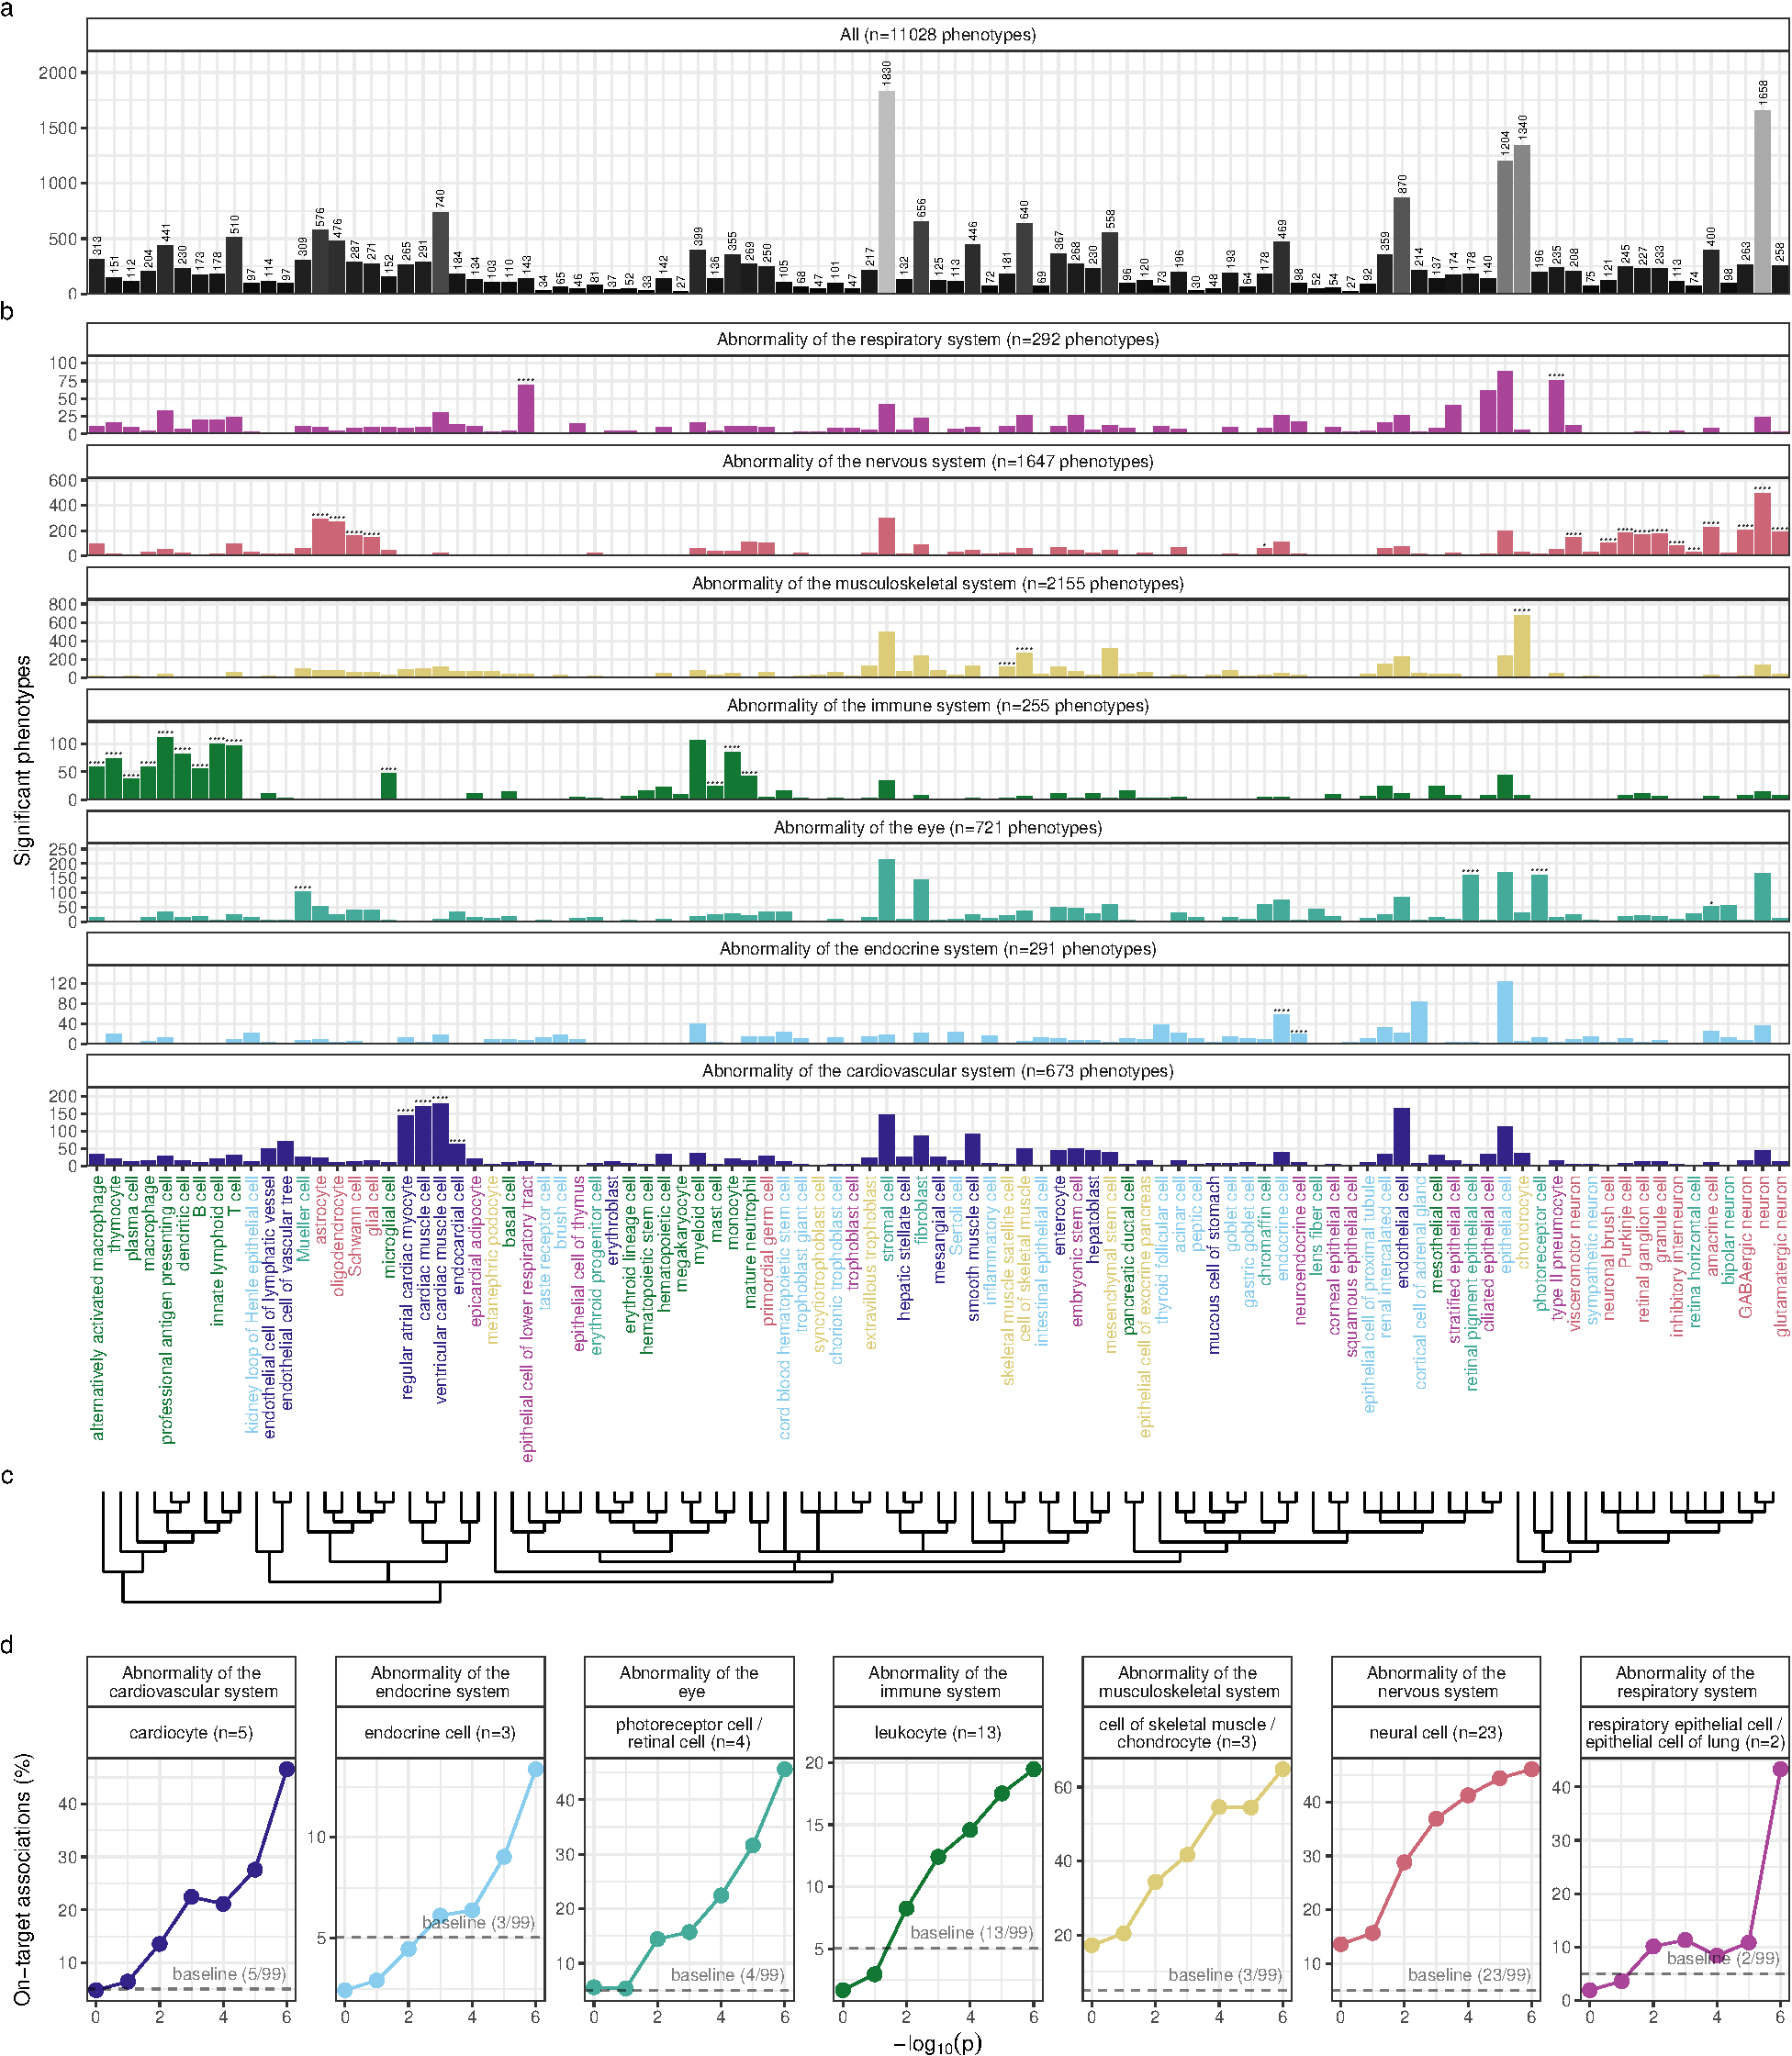
\includegraphics{index_files/figure-pdf/fig-summary-1.pdf}

}

\caption{\label{fig-summaryD08295A6-16DC-499D-85A8-8BA656E013A2}High-throughput
analysis reveals cell types underlying thousands of rare disease
phenotypes. \textbf{a}, Some cell types are much more commonly
associated with phenotypes than others. Bar height indicates the total
number of significant phenotype enrichments per cell type (\(FDR<0.05\))
across all branches of the HPO. \textbf{b}, Analyses reveal expected and
novel cell type associations within high-level HPO branches. Asterisks
above each bar indicate whether that cell type was significantly more
often enriched in that branch relative to all other HPO branches,
including those not shown here, as a proxy for how specifically that
cell type is associated with that branch; FDR\textless0.0001 (****),
FDR\textless0.001 (***), FDR\textless0.01 (**), FDR\textless0.05 (*).
\textbf{c}, Ontological relatedness of cell types in the Cell Ontology
(CL)\textsuperscript{34}. \textbf{d}, The proportion of on-target
associations (\emph{y-axis}) increases with greater test significance
(\emph{x-axis}). Percentage of significant phenotype associations with
on-target cell types (second row of facet labels), respective to the HPO
branch.}

\end{figure}%

\subsection{Validation of inter- and intra-dataset
consistency}\label{validation-of-inter--and-intra-dataset-consistency}

Next, we sought to validate the consistency of our results across the
two single-cell reference datasets (Descartes Human vs.~Human Cell
Landscape) across the subset of overlapping cell types
\textbf{?@fig-ctd-correlation}. In total there were 142,285
phenotype-cell type associations to compare across the two datasets
(across 10,945 phenotypes and 13 cell types annotated to the exact same
CL term. We found that the correlation between p-values of the two
datasets was high (\(rho\)=\(0.49\), \(p\)=\(1.1 \times 10^{-93}\)).
Within the subset of results that were significant in both single-cell
datasets (FDR\textless0.05), we found that correlation of the
association effect size were even stronger (\(rho=\)\(0.72\),
\(p=\)\(1.1 \times 10^{-93}\)). We also checked for the intra-dataset
consistency between the p-values of the foetal and adult samples in the
Human Cell Landscape, showing a very similar degree of correlation as
the inter-dataset comparison (\(rho=\)\(0.44\),
\(p=\)\(2.4 \times 10^{-149}\)). Together, these results suggest that
our approach to identifying phenotype-cell type associations is highly
replicable and generalisable to new datasets.

\subsection{More specific phenotypes are associated with fewer genes and
cell
types}\label{more-specific-phenotypes-are-associated-with-fewer-genes-and-cell-types}

Higher levels of the ontology are broad classes of phenotype
(e.g.~`Abnormality of the nervous system') while the lower levels can
get very detailed (e.g.~`Spinocerebellar atrophy'). The higher level
phenotypes inherit all genes associated with lower level phenotypes, so
naturally they have more genes than the lower level phenotypes
(\textbf{?@fig-ontology-lvl}a; \(rho=\)\(-0.26\),
\(p=\)\(2.2 \times 10^{-308}\)).

Next, we reasoned that the more detailed and specific a phenotype is,
the more likely it is to be driven by one cell type. For example, while
`Neurodevelopmental abnormality' could plausibly be driven by any/all
cell types in the brain, it is more likely that `Impaired visuospatial
constructive cognition' is driven by a single cell type. This was indeed
the case, as we observed a strongly significant negative correlation
between the two variables (\textbf{?@fig-ontology-lvl}b;
\(rho=\)\(-0.29\), \(p=\)\(2.2 \times 10^{-308}\)). We also found that
the phenotype-cell type association p-values increased with greater
phenotype specificity, reflecting the decreasing overall number of
associated cell types at each ontological level
(\textbf{?@fig-ontology-lvl}c; \(rho=\)\(0.26\),
\(p=\)\(2.2 \times 10^{-308}\)).

\begin{figure}[H]

\centering{

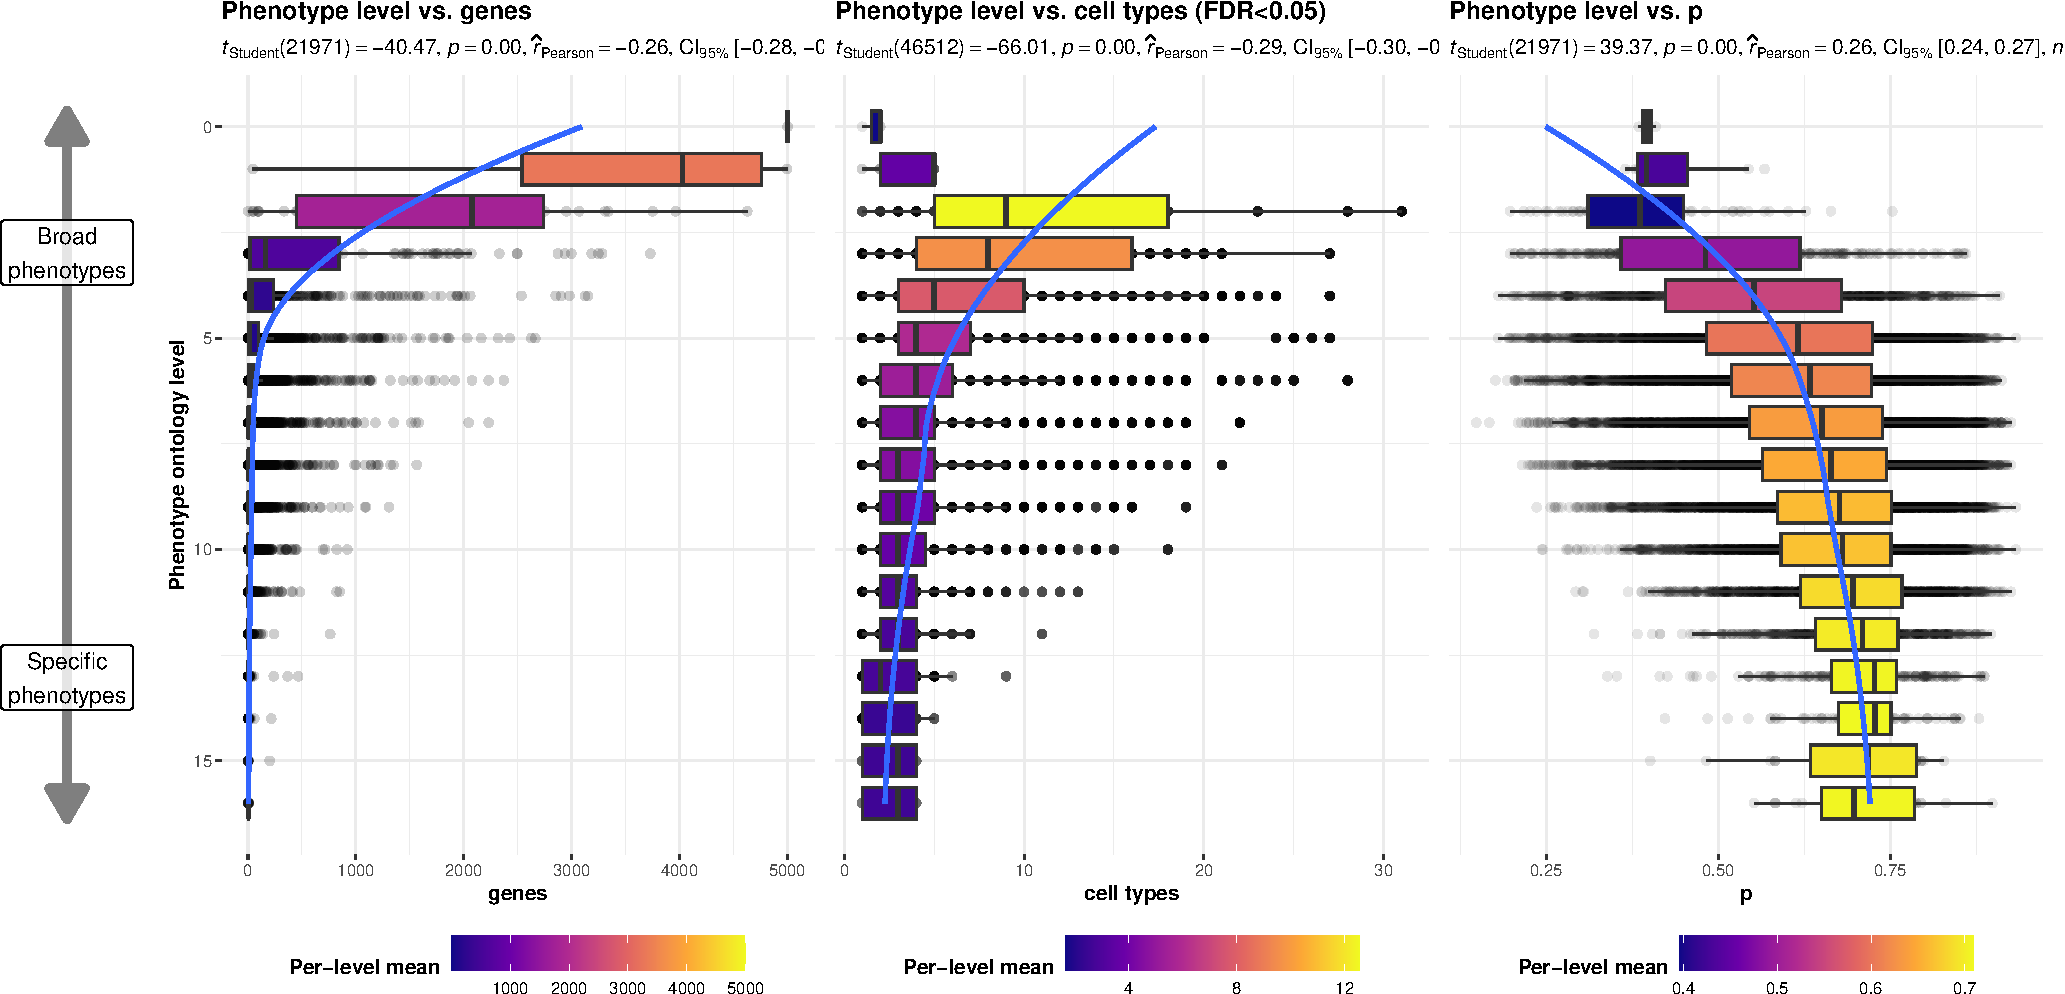
\includegraphics{index_files/figure-pdf/fig-ontology-lvl-1.pdf}

}

\caption{\label{fig-ontology-lvlD08295A6-16DC-499D-85A8-8BA656E013A2}More
specific phenotypes are associated with fewer, more specific genes and
cell types. Box plots showing relationship between HPO phenotype level
and \textbf{a}, the number of genes annotated to each phenotype,
\textbf{b}, the number of significantly enriched cell types, \textbf{c},
the p-values of phenotype-cell type association tests. Ontology level 0
represents the most inclusive HPO term `All', while higher ontology
levels (max=16) indicate progressively more specific HPO terms
(e.g.~`Contracture of proximal interphalangeal joints of 2nd-5th
fingers'). Boxes are coloured by the mean value (respective to the
subplot) within each HPO level.}

\end{figure}%

\subsection{Hepatoblasts have a unique role in recurrent Neisserial
infections}\label{hepatoblasts-have-a-unique-role-in-recurrent-neisserial-infections}

We selected the HPO term `Recurrent bacterial infections' and all of its
descendants (\(19\) phenotypes) as an example of how investigations at
the level of granular phenotypes can reveal different cell type-specific
mechanisms (\textbf{?@fig-rni}). As expected, these phenotypes are
primarily associated with immune cell types (e.g.~macrophages, dendritic
cells, T cells, monocytes, neutrophils). Some associations confirm
relationships previously suggested in the literature, such as that
between `Recurrent staphylococcal infections' and myeloid
cells\textsuperscript{35--38}. Specifically, our results pinpoint
monocytes as the most strongly associated cell subtypes
(FDR=\(1.0 \times 10^{-30}\), \(\beta\)=\(0.18\)).

In contrast to all other recurrent infection types, `Recurrent
Neisserial infections' highlighted a novel association with hepatoblasts
(Descartes Human : FDR=\(1.1 \times 10^{-6}\),
\(\beta\)=\(8.2 \times 10^{-2}\)). Whilst unexpected, a convincing
explanation involves the complement system, a key driver of innate
immune response to Neisserial infections. Hepatocytes, which derive from
hepatoblasts, produce the majority of complement
proteins\textsuperscript{39}, and Kupffer cells express complement
receptors\textsuperscript{40}. In addition, individuals with deficits in
complement are at high risk for Neisserial
infections\textsuperscript{41,42}, and a genome-wide association study
in those with a Neisserial infection identified risk variants within
complement proteins\textsuperscript{43} . While the potential of
therapeutically targeting complement in RDs (including Neisserial
infections) has been proposed previously\textsuperscript{44,45},
performing this in a gene- and cell type-specific manner may help to
improve efficacy and reduce toxicity (e.g.~due to off-target effects).
Importantly, there are over 56 known genes within the complement
system\textsuperscript{46}, highlighting the need for a systematic,
evidence-based approach to identify effective gene targets.

Also of note, despite the fact that our datasets contain both
hepatoblasts and their mature counterpart, hepatocytes, only the
hepatoblasts showed this association. This suggests that the genetic
factors that predispose individuals for risk of Neisserial infections
are specifically affecting hepatoblasts before they become fully
differentiated. It is also notable that these phenotypes were the only
ones within the `Recurrent bacterial infections' branch, or even the
broader `Recurrent infections' branch, perhaps indicating a unique role
for hepatoblasts in recurrent infectious disease. The only phenotypes
within the even broader `Abnormality of the immune system' HPO branch
that significantly associated with mature hepatocytes were
`Pancreatitis' (FDR=\(2.1 \times 10^{-2}\),
\(\beta\)=\(5.3 \times 10^{-2}\)) and `Susceptibility to chickenpox'
(FDR=\(1.2 \times 10^{-2}\), \(\beta\)=\(5.5 \times 10^{-2}\)) both of
which are well-known to involve the liver\textsuperscript{47--49}.

\begin{figure}[H]

\centering{

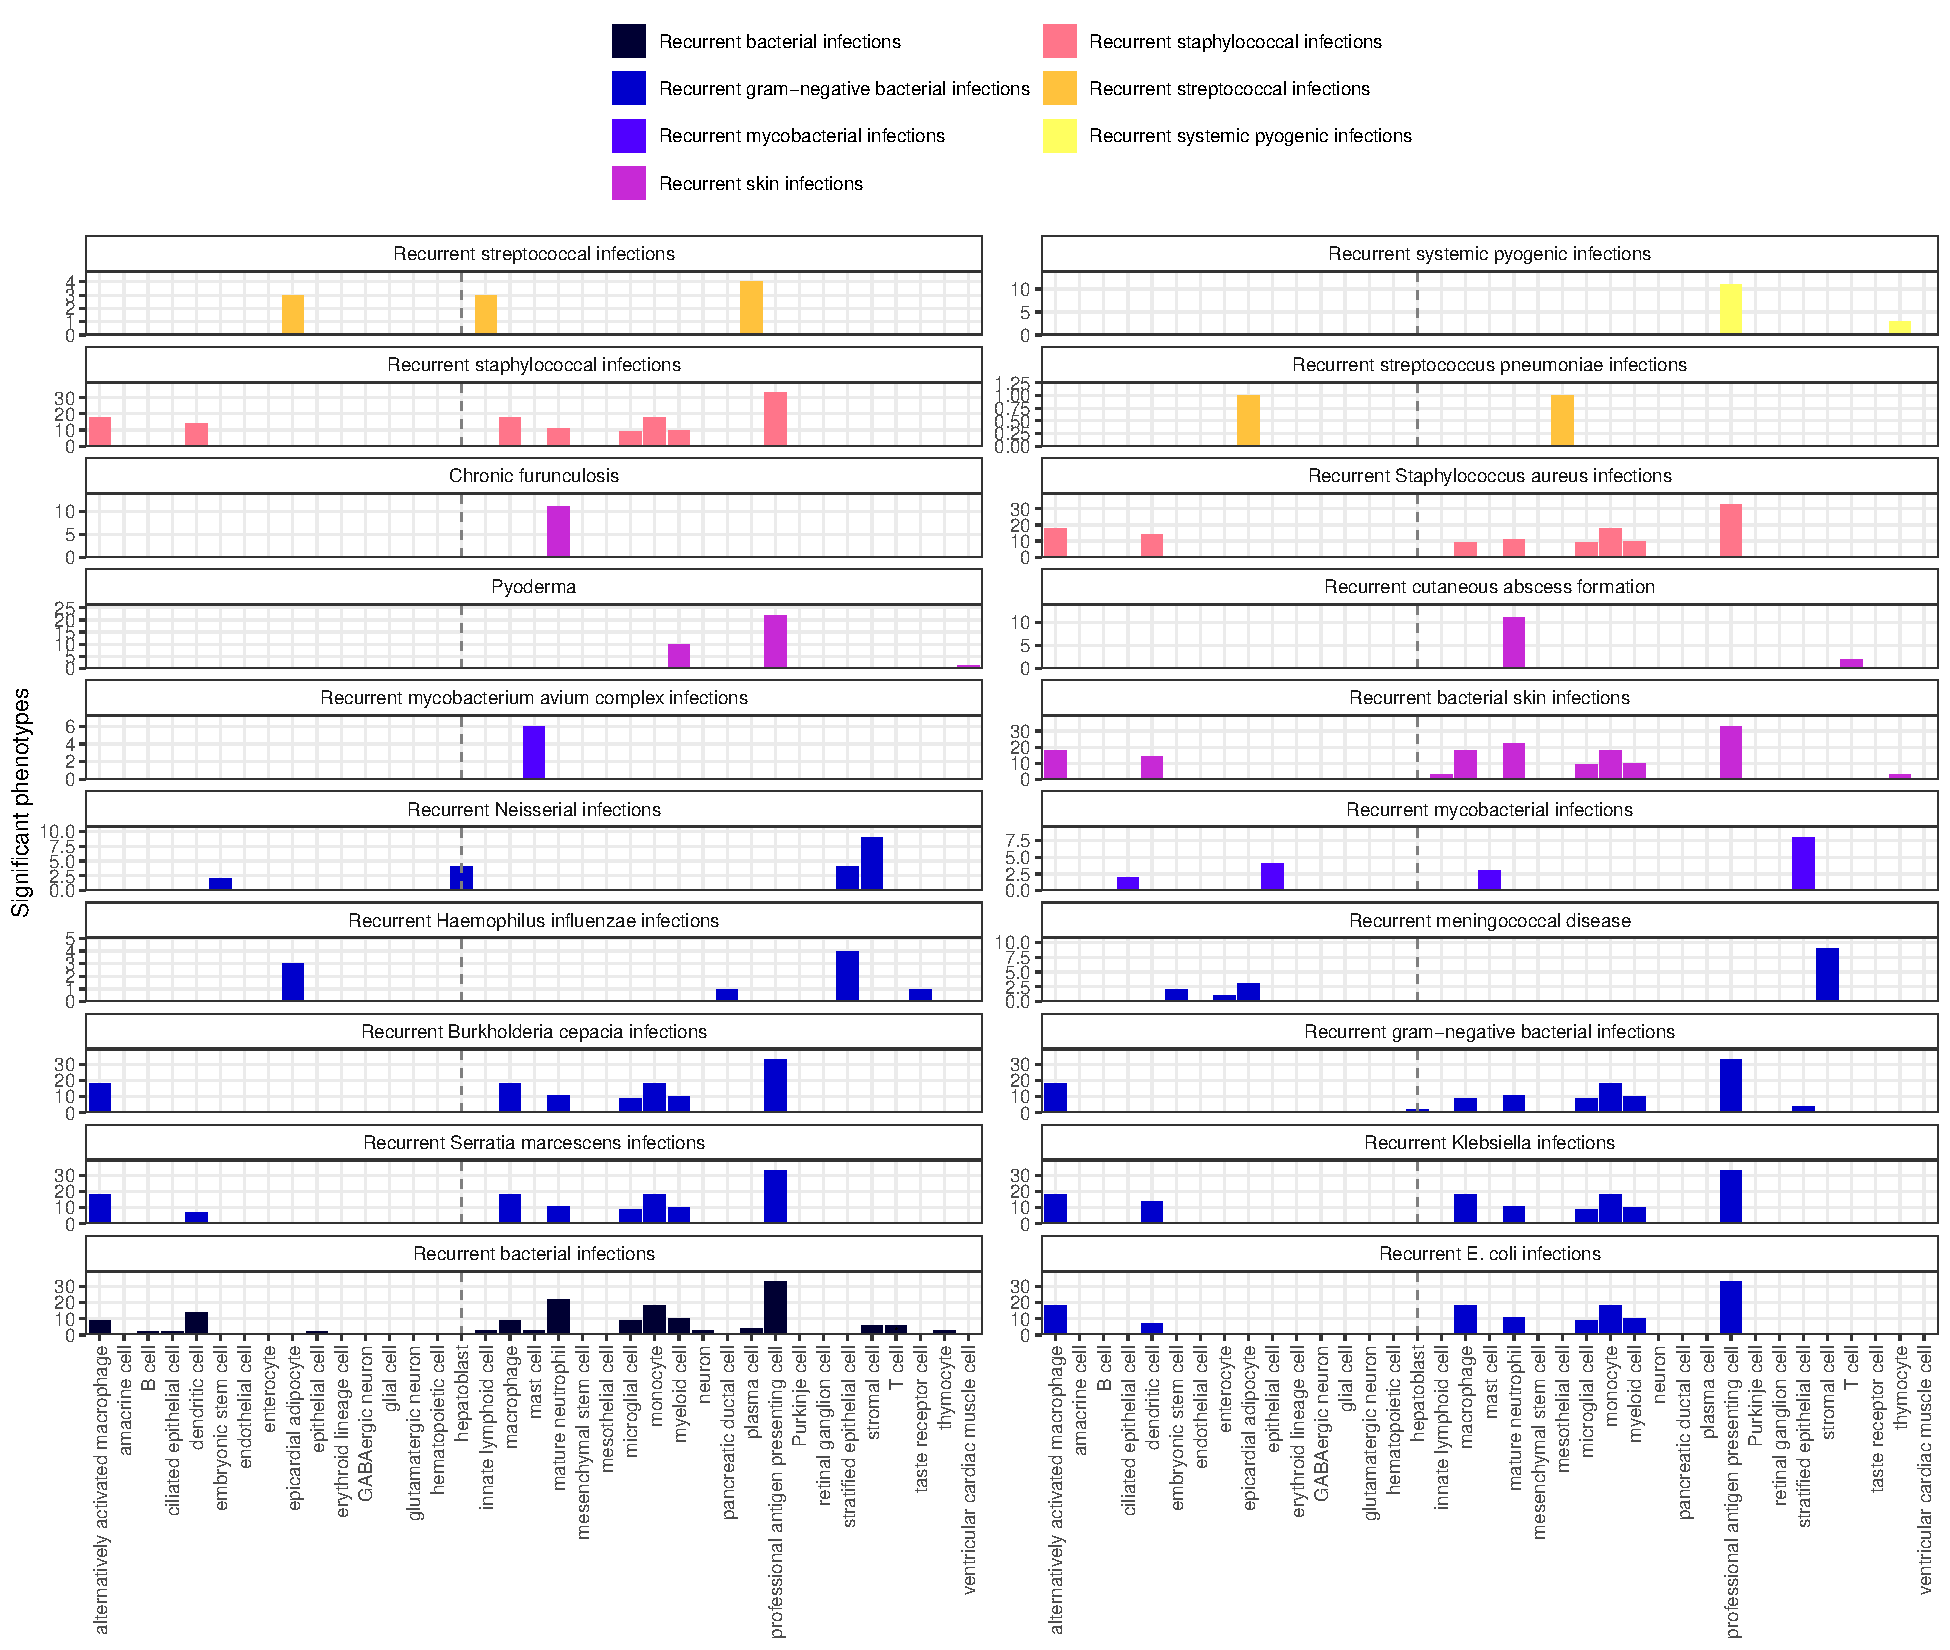
\includegraphics{index_files/figure-pdf/fig-rni-1.pdf}

}

\caption{\label{fig-rniD08295A6-16DC-499D-85A8-8BA656E013A2}Hepatoblasts
have a unique role in recurrent Neisserial infections. Significant
phenotype-cell type tests for phenotypes within the branch `Recurrent
bacterial infections'. Amongst all different kinds of recurrent
bacterial infections, hepatoblasts (highlighted by vertical dotted
lines) are exclusively enriched in `Recurrent gram−negative bacterial
infections'. Note that terms from multiple levels of the same ontology
branch are shown as separate facets (e.g.~`Recurrent bacterial
infections' and `Recurrent gram−negative bacterial infections').}

\end{figure}%

Phenotypes can be associated with multiple diseases, cell types and
genes. In addition to hepatoblasts, `Recurrent Neisserial infections'
were also associated with stromal cells (FDR=\(4.6 \times 10^{-6}\),
\(\beta\)=\(7.9 \times 10^{-2}\)), stratified epithelial cells
(FDR=\(1.7 \times 10^{-23}\), \(\beta\)=\(0.15\)), and embryonic stem
cells (FDR=\(5.4 \times 10^{-5}\), \(\beta\)=\(7.4 \times 10^{-2}\)).
RNI is a phenotype of 7 different diseases (`C5 deficiency', `C6
deficiency', `C7 deficiency', `Complement component 8 deficiency, type
II', `Complement factor B deficiency', `Complement factor I deficiency',
`Mannose-Binding lectin deficiency').

Next, we sought to link multi-scale mechanisms at the levels of disease,
phenotype, cell type, and gene and visualise these as a network
(\textbf{?@fig-network-rni}). This revealed that genetic deficiencies in
different complement system genes (e.g.~\emph{C5}, \emph{C8}, and
\emph{C7}) are primarily mediated by different cell types (hepatoblasts,
stratified epithelial cells, and stromal cells, respectively). While
genes of the complement system are expressed throughout many different
tissues and cell types, these results indicate that different subsets of
these genes may mediate their effects through different cell types. This
finding suggests that investigating (during diagnosis) and targeting
(during treatment) different cell types may be critical for the
diagnosis and treatment of these closely related, yet mechanistically
distinct, diseases.

\begin{figure}[H]

\centering{

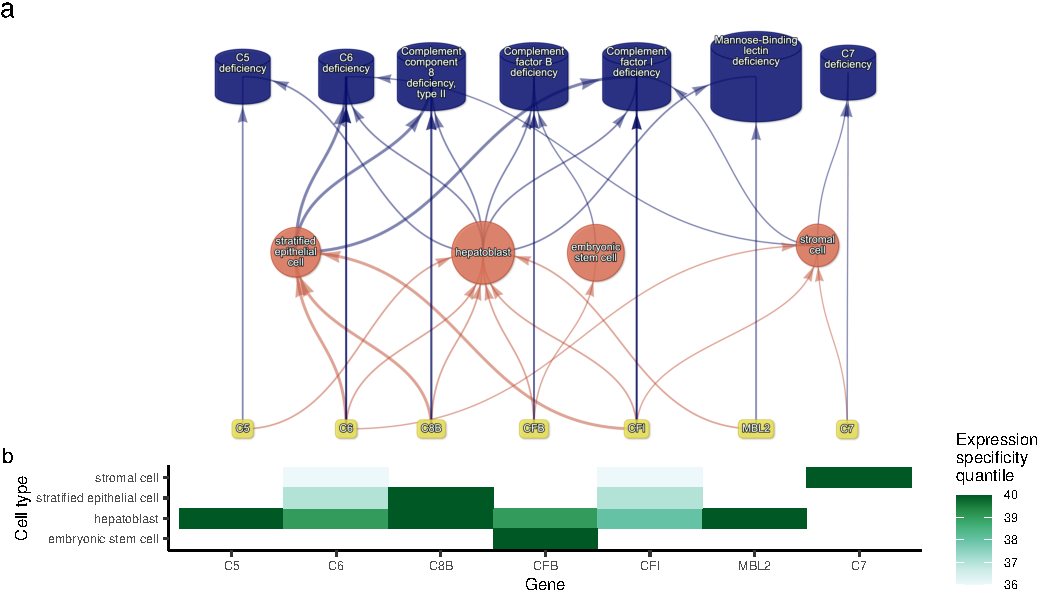
\includegraphics{index_files/figure-pdf/fig-network-rni-1.pdf}

}

\caption{\label{fig-network-rniD08295A6-16DC-499D-85A8-8BA656E013A2}Multi-scale
mechanisms of Recurrent Neisserial infections. Starting from the bottom
of the plot, one can trace how causal genes (yellow boxes) mediate their
effects through cell types (orange circles), phenotypes (purple
cylinders) and ultimately diseases (blue cylinders). Cell types are
connected to phenotypes via association testing (FDR\textless0.05), and
to diseases when the symptom gene set overlap is \textgreater25\%. Only
the top driver genes (specificity quantiles\textgreater75\%) mediating
each phenotype-cell type association are shown. Nodes were spatially
arranged using the Sugiyama algorithm\textsuperscript{50}.}

\end{figure}%

\subsection{Monarch Knowledge Graph
recall}\label{monarch-knowledge-graph-recall}

Next, we used the Monarch Knowledge Graph (MKG) as a proxy for the
field's current state of knowledge of phenotype-cell type associations.
We evaluated the proportion of MKG associations that were recapitulation
by our results \textbf{?@fig-monarch-recall}. For each phenotype-cell
type association in the MKG, we computed the percent of cell types
recovered in our association results at a given ontological distance
according to the CL ontology. An ontological distance of 0 means that
our nominated cell type was as close as possible to the MKG cell type
after adjusting for the cell types available in our single-cell
references. Instances of exact overlap of terms between the MKG and our
results would qualify as an ontological distance of 0 (e.g.~`monocyte'
vs.~`monocyte'). Greater ontological distances indicate further
divergence between the MKG cell type and our nominated cell type. A
distance of 1 indicating that the MKG cell type was one step away from
our nominated cell type in the CL ontology graph (e.g.~`monocyte'
vs.~`classical monocyte'). The maximum possible percent of recovered
terms is capped by the percentage of MKG ground-truth phenotypes we were
able to find at least one significant cell type association for at
\(FDR_{pc}\).

In total, our results contained at least one significant cell type
associations for \(90\)\% of the phenotypes described in the MKG. Of
these phenotypes, we captured \(55\)\% of the MKG phenotype-cell
associations at an ontological distance of 0 (i.e.~the closest possible
Cell Ontology term match). Recall increased with greater flexibility in
the matching of cell type annotations. At an ontological distance of 1
(e.g.~`monocyte' vs.~`classical monocyte'), we captured \(77\)\% of the
MKG phenotype-cell associations. Recall reached a maximum of \(90\)\% at
a ontological distance of 5. This recall percentage is capped by the
proportion of phenotype for which we were able to find at least one
significant cell type association for. It should be noted that we were
unable to compute precision as the MKG (and other knowledge databases)
only provide true positive associations. Identifying true negatives
(e.g.~a cell type is definitely never associated with a phenotype) is a
fundamentally more difficult task to resolve as it would require proving
the null hypothesis. Regardless, these benchmarking tests suggests that
our results are able to recover the majority of known phenotype-cell
type associations while proposing many new associations.

\subsection{Annotation of phenotypes using generative large language
models}\label{annotation-of-phenotypes-using-generative-large-language-models}

Severity annotations were gathered from GPT-4 for 16,982/18,082
(\(94\)\%) HPO phenotypes in our companion study\textsuperscript{32}.
Benchmarking tests of these results using ground-truth HPO branch
annotations. For example, phenotypes within the `Blindness' HPO branch
(\emph{HP:0000618}) were correctly annotated as causing blindness by
GPT-4. Across all annotations, the recall rate of GPT-4 annotations was
\(96\)\% (min=\(89\)\%, max=\(100\)\%, SD=\(4.5\)) with a mean
consistency score of \(91\)\% (min=\(81\)\%, max=\(97\)\%, SD=\(5.7\))
for phenotypes whose annotation were collected more than once. This
clearly demonstrates the ability of GPT-4 to accurately annotate
phenotypes. This allowed us to begin using these annotations to compute
systematically collected severity scores for all phenotypes in the HPO.

From these annotations we computed a weighted severity score metric for
each phenotype ranging from 0-100 (100 being the theoretical maximum
severity of a phenotype that always causes every annotation). Within our
annotations, the most severe phenotype was `Atrophy/Degeneration
affecting the central nervous system' (\emph{HP:0007367}) with a
severity score of \(47\), followed by `Anencephaly' (\emph{HP:0002323})
with a severity score of \(45\). There were 677 phenotypes with a
severity score of 0 (e.g.~`Thin toenail'). The mean severity score
across all phenotypes was \(10\) (median=\(9.4\), standard
deviation=\(6.4\)).

\subsection{Congenital phenotypes are associated with foetal cell
types}\label{congenital-phenotypes-are-associated-with-foetal-cell-types}

To further verify the biological relevance of our results, we examined
the association of foetal cell types with phenotypes annotated as
congenital in onset. As expected, the frequency of congenital onset with
each phenotype (as determined by GPT-4 annotations) was strongly
predictive with the proportion of significantly associated foetal cell
types in our results (\(p=\)\(2.0 \times 10^{-203}\),
\(\chi^2_{Pearson}=\)\(940\), \(\hat{V}_{Cramer}=\)\(0.14\)).
Furthermore, increasing congenital frequency annotation (on an ordinal
scale) corresponded to an increase in the proportion of foetal cell
types: `always'=24\% (n=1636 associations), `often'=20\% (n=2979
associations), `rarely'=12\% (n=1956 associations), `never'=10\% (n=811
associations). This is consistent with the expected role of foetal cell
types in development and the aetiology of congenital disorders.

\begin{figure}[H]

\centering{

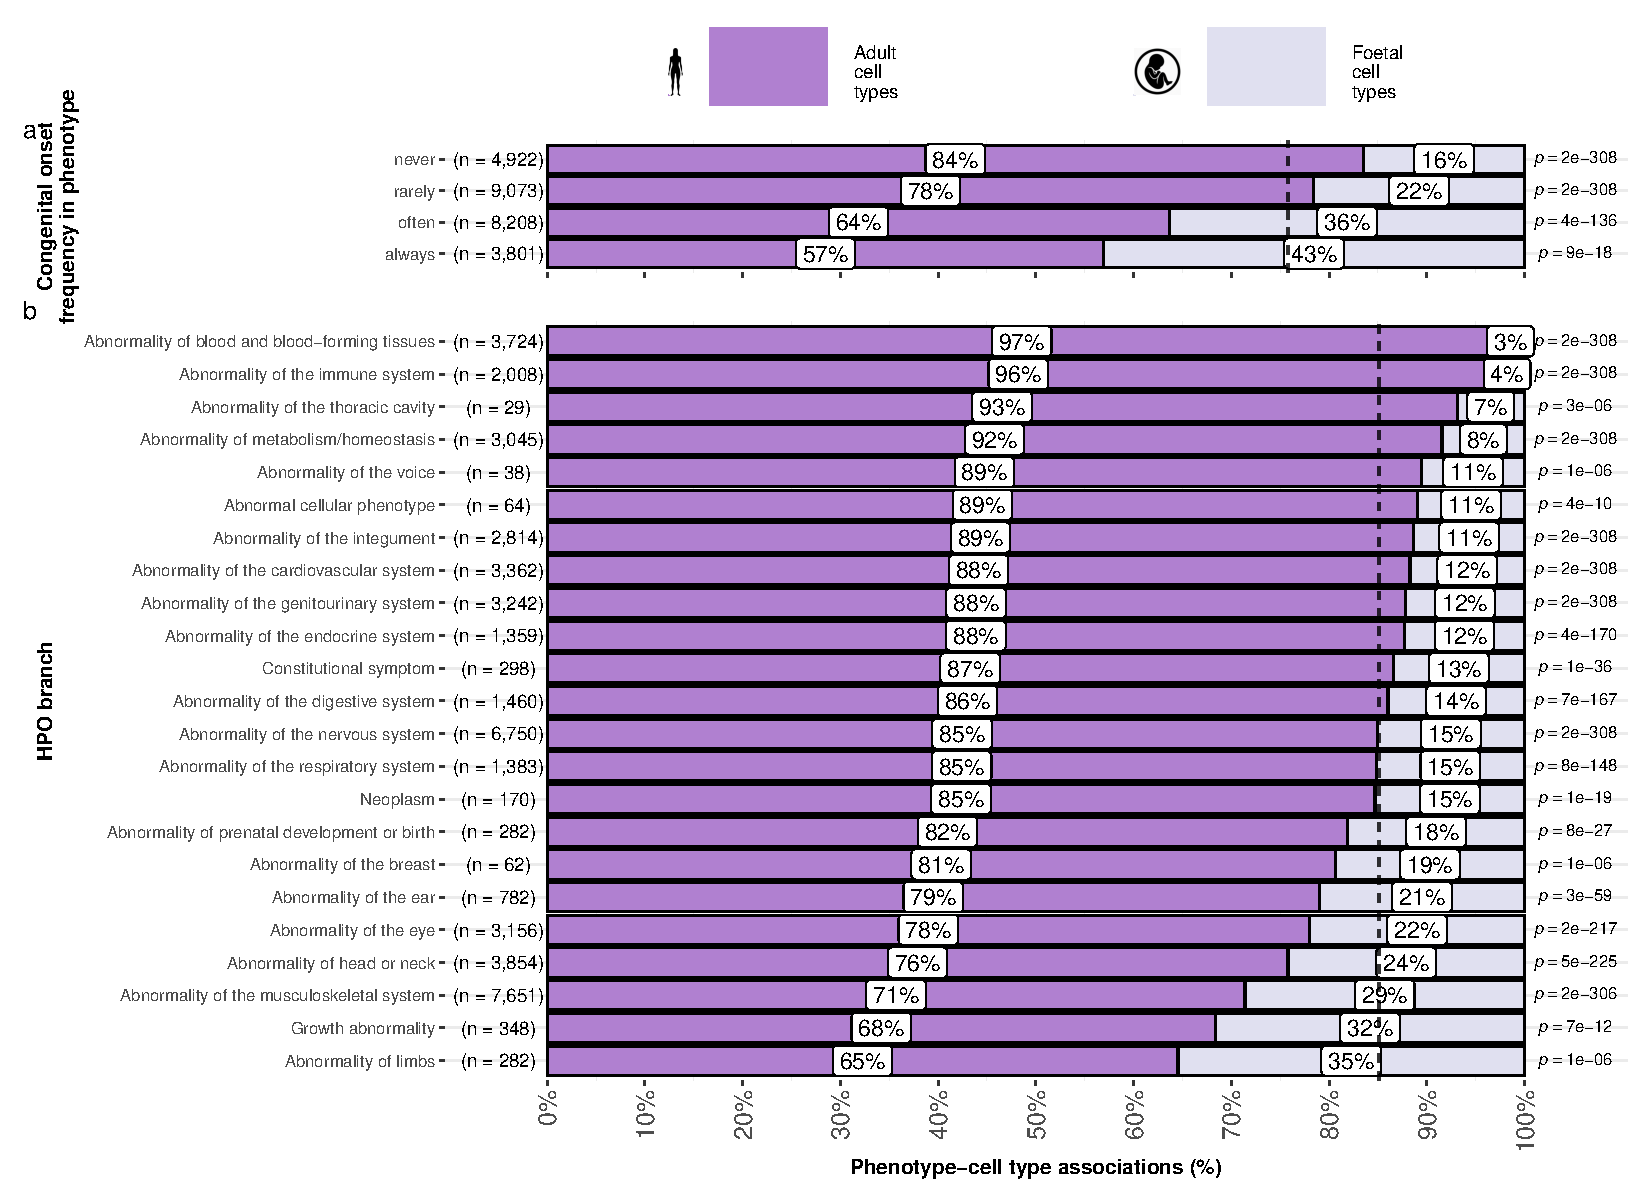
\includegraphics{index_files/figure-pdf/fig-congenital-1.pdf}

}

\caption{\label{fig-congenitalD08295A6-16DC-499D-85A8-8BA656E013A2}Congenital
phenotypes are more often associated with foetal cell types. As a
phenotype is more often congenital in nature, the greater proportion of
foetal cell types are significantly associated with it. The summary
statistics in the plot title are the results of a \(\chi^2\) tests of
independence between the ordinal scale of congenital onset and the
proportion of foetal cell types associated with each phenotype. The
p-values above each bar are the results of an additional series of
\(\chi^2\) tests to determine whether the proportion of foetal
vs.~non-foetal cell types significantly different differs from the
proprortions expected by chance. The feotal silhouette was generated
with DALL-E. The adult silhouette is from phylopic.org and is freely
available via CC0 1.0 Universal Public Domain Dedication.}

\end{figure}%

We also found that some branches of the HPO were more commonly enriched
in foetal cell types compared to others (\(\hat{V}_{Cramer}\)=\(0.22\),
\(p\)\textless{}\(2.2 \times 10^{-308}\)). See The branch with the
greatest proportion of fetal cell type enrichments was `Abnormality of
limbs' (\(35\)\%), followed by `Growth abnormality' (\(32\)\%) and
`Abnormality of the musculoskeletal system' (\(29\)\%). These results
align well with the fact that physical malformations tend to be
developmental in origin.

\subsection{Therapeutic target
identification}\label{therapeutic-target-identification}

Next, we identified putative cell type-specific gene targets for several
severe disease phenotypes. This yielded putative therapeutic targets for
5,252 phenotypes across 4,823 diseases in 201 cell types and 3,150 genes
(\textbf{?@fig-therapy-filter}). While this constitutes a large number
of genes in total, each phenotype was assigned a median of \(2.0\) gene
targets (mean=\(3.3\), min=1, max=10). Relative to the number of genes
annotations per phenotype in the HPO overall (median=\(7.0\),
mean=\(62\), min=1, max=5,003) this represents a substantial decrease in
the number of candidate target genes, even when excluding high-level
phenotypes (HPO level\textgreater{}\(3.0\)). It is also important to
note that the phenotypes in the prioritised targets list are ranked by
their severity, allowing us to distinguish between phenotypes with a
high medical urgency (e.g.~`Hydranencephaly') from those with lower
medical urgency (e.g.~`Hyperplastic labia majora'). This can be useful
for both clinicians, biomedical scientists, and pharmaceutical
manufacturers who wish to focus their research efforts on phenotypes
with the greatest need for intervention.

Across all phenotypes, epithelial cell were most commonly implicated
(838 phenotypes), followed by stromal cell (627 phenotypes), stromal
cell (627 phenotypes), neuron (475 phenotypes), chondrocyte (383
phenotypes), and endothelial cell (361 phenotypes). Grouped by
higher-order ontology category, `Abnormality of the musculoskeletal
system' had the greatest number of enriched phenotypes (959 phenotypes,
857 genes), followed by `Abnormality of the nervous system' (733
phenotypes, 1,137 genes), `Abnormality of head or neck' (543 phenotypes,
990 genes), `Abnormality of the genitourinary system' (443 phenotypes,
696 genes), and `Abnormality of the eye' (377 phenotypes, 548 genes).

\subsection{Therapeutic target
validation}\label{therapeutic-target-validation}

To determine whether the genes prioritised by our therapeutic targets
pipeline were plausible, we checked what percentage of gene therapy
targets we recapitulated. Data on therapeutic approval status was
gathered from the Therapeutic Target Database (TTD; release
2024-07-23)\textsuperscript{51}. Overall, we prioritised \(81\)\% of all
non-failed existing gene therapy targets. A hypergeometric test
confirmed that our prioritised targets were significantly enriched for
non-failed gene therapy targets (\(p=\)\(1.8 \times 10^{-3}\)).
Importantly, we did not prioritise any of the failed therapeutics (0\%),
defined as having been terminated or withdrawn from the market. The
hypergeometric test for depletion of failed targets did not reach
significance (\(p=\)\(0.37\)), but this is to be expected as there was
only one failed gene therapy target in the TTD database.

Even when considering therapeutics of any kind
(\textbf{?@fig-therapy-validate-all}), not just gene therapies, we
recapitulated \(40\)\% of the non-failed therapeutic targets and 0\% of
the terminated/withdrawn therapeutic targets (n=1,255). Here we found
that our prioritised targets were highly significantly depleted for
failed therapeutics (\(p=\)\(3.9 \times 10^{-196}\)). This suggests that
our multi-scale evidence-based prioritisation pipeline is capable of
selectively identifying genes that are likely to be effective
therapeutic targets.

\begin{figure}[H]

\centering{

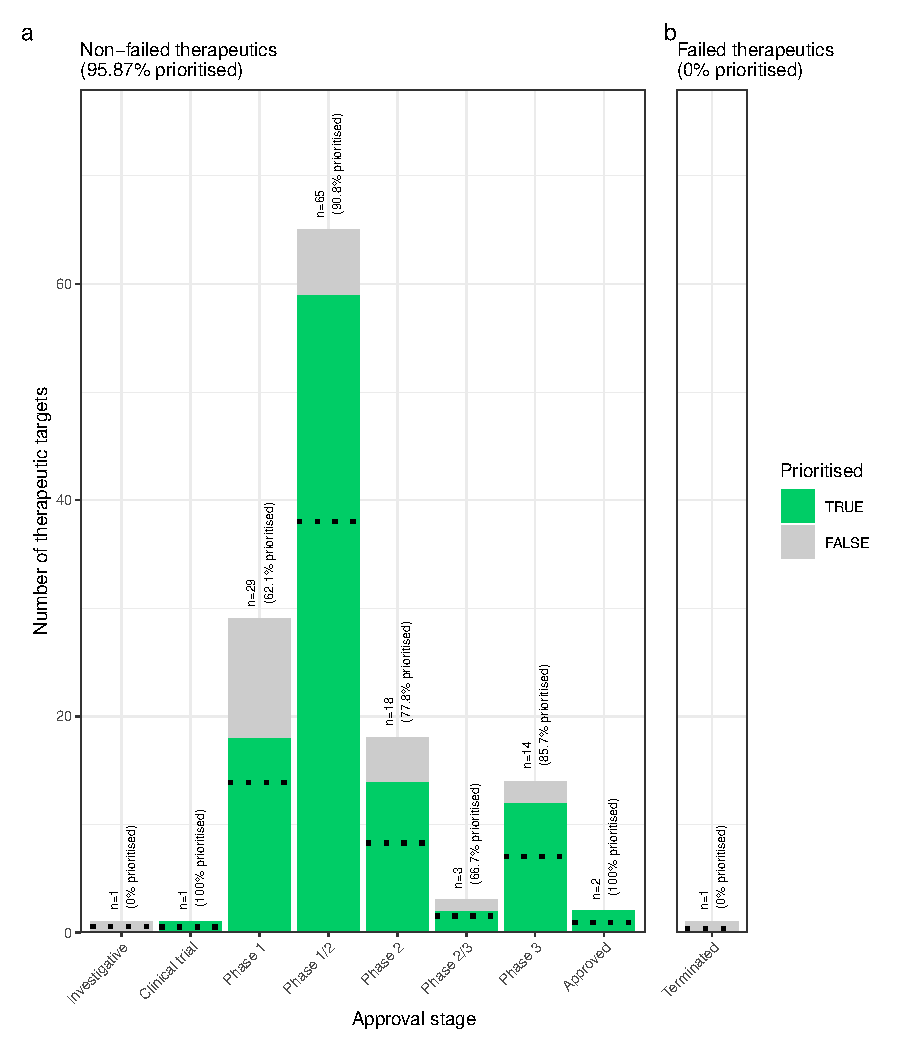
\includegraphics{index_files/figure-pdf/fig-therapy-validate-1.pdf}

}

\caption{\label{fig-therapy-validateD08295A6-16DC-499D-85A8-8BA656E013A2}Validation
of prioritised therapeutic targets. The proportion of existing gene
therapy targets (documented in the Therapeutic Target Database)
recapitulated by our prioritisation pipeline. Therapetics are stratified
by the stage of clinical development they were at during the time of
writing.}

\end{figure}%

\subsection{Selected example targets}\label{selected-example-targets}

\begin{figure}[H]

\centering{

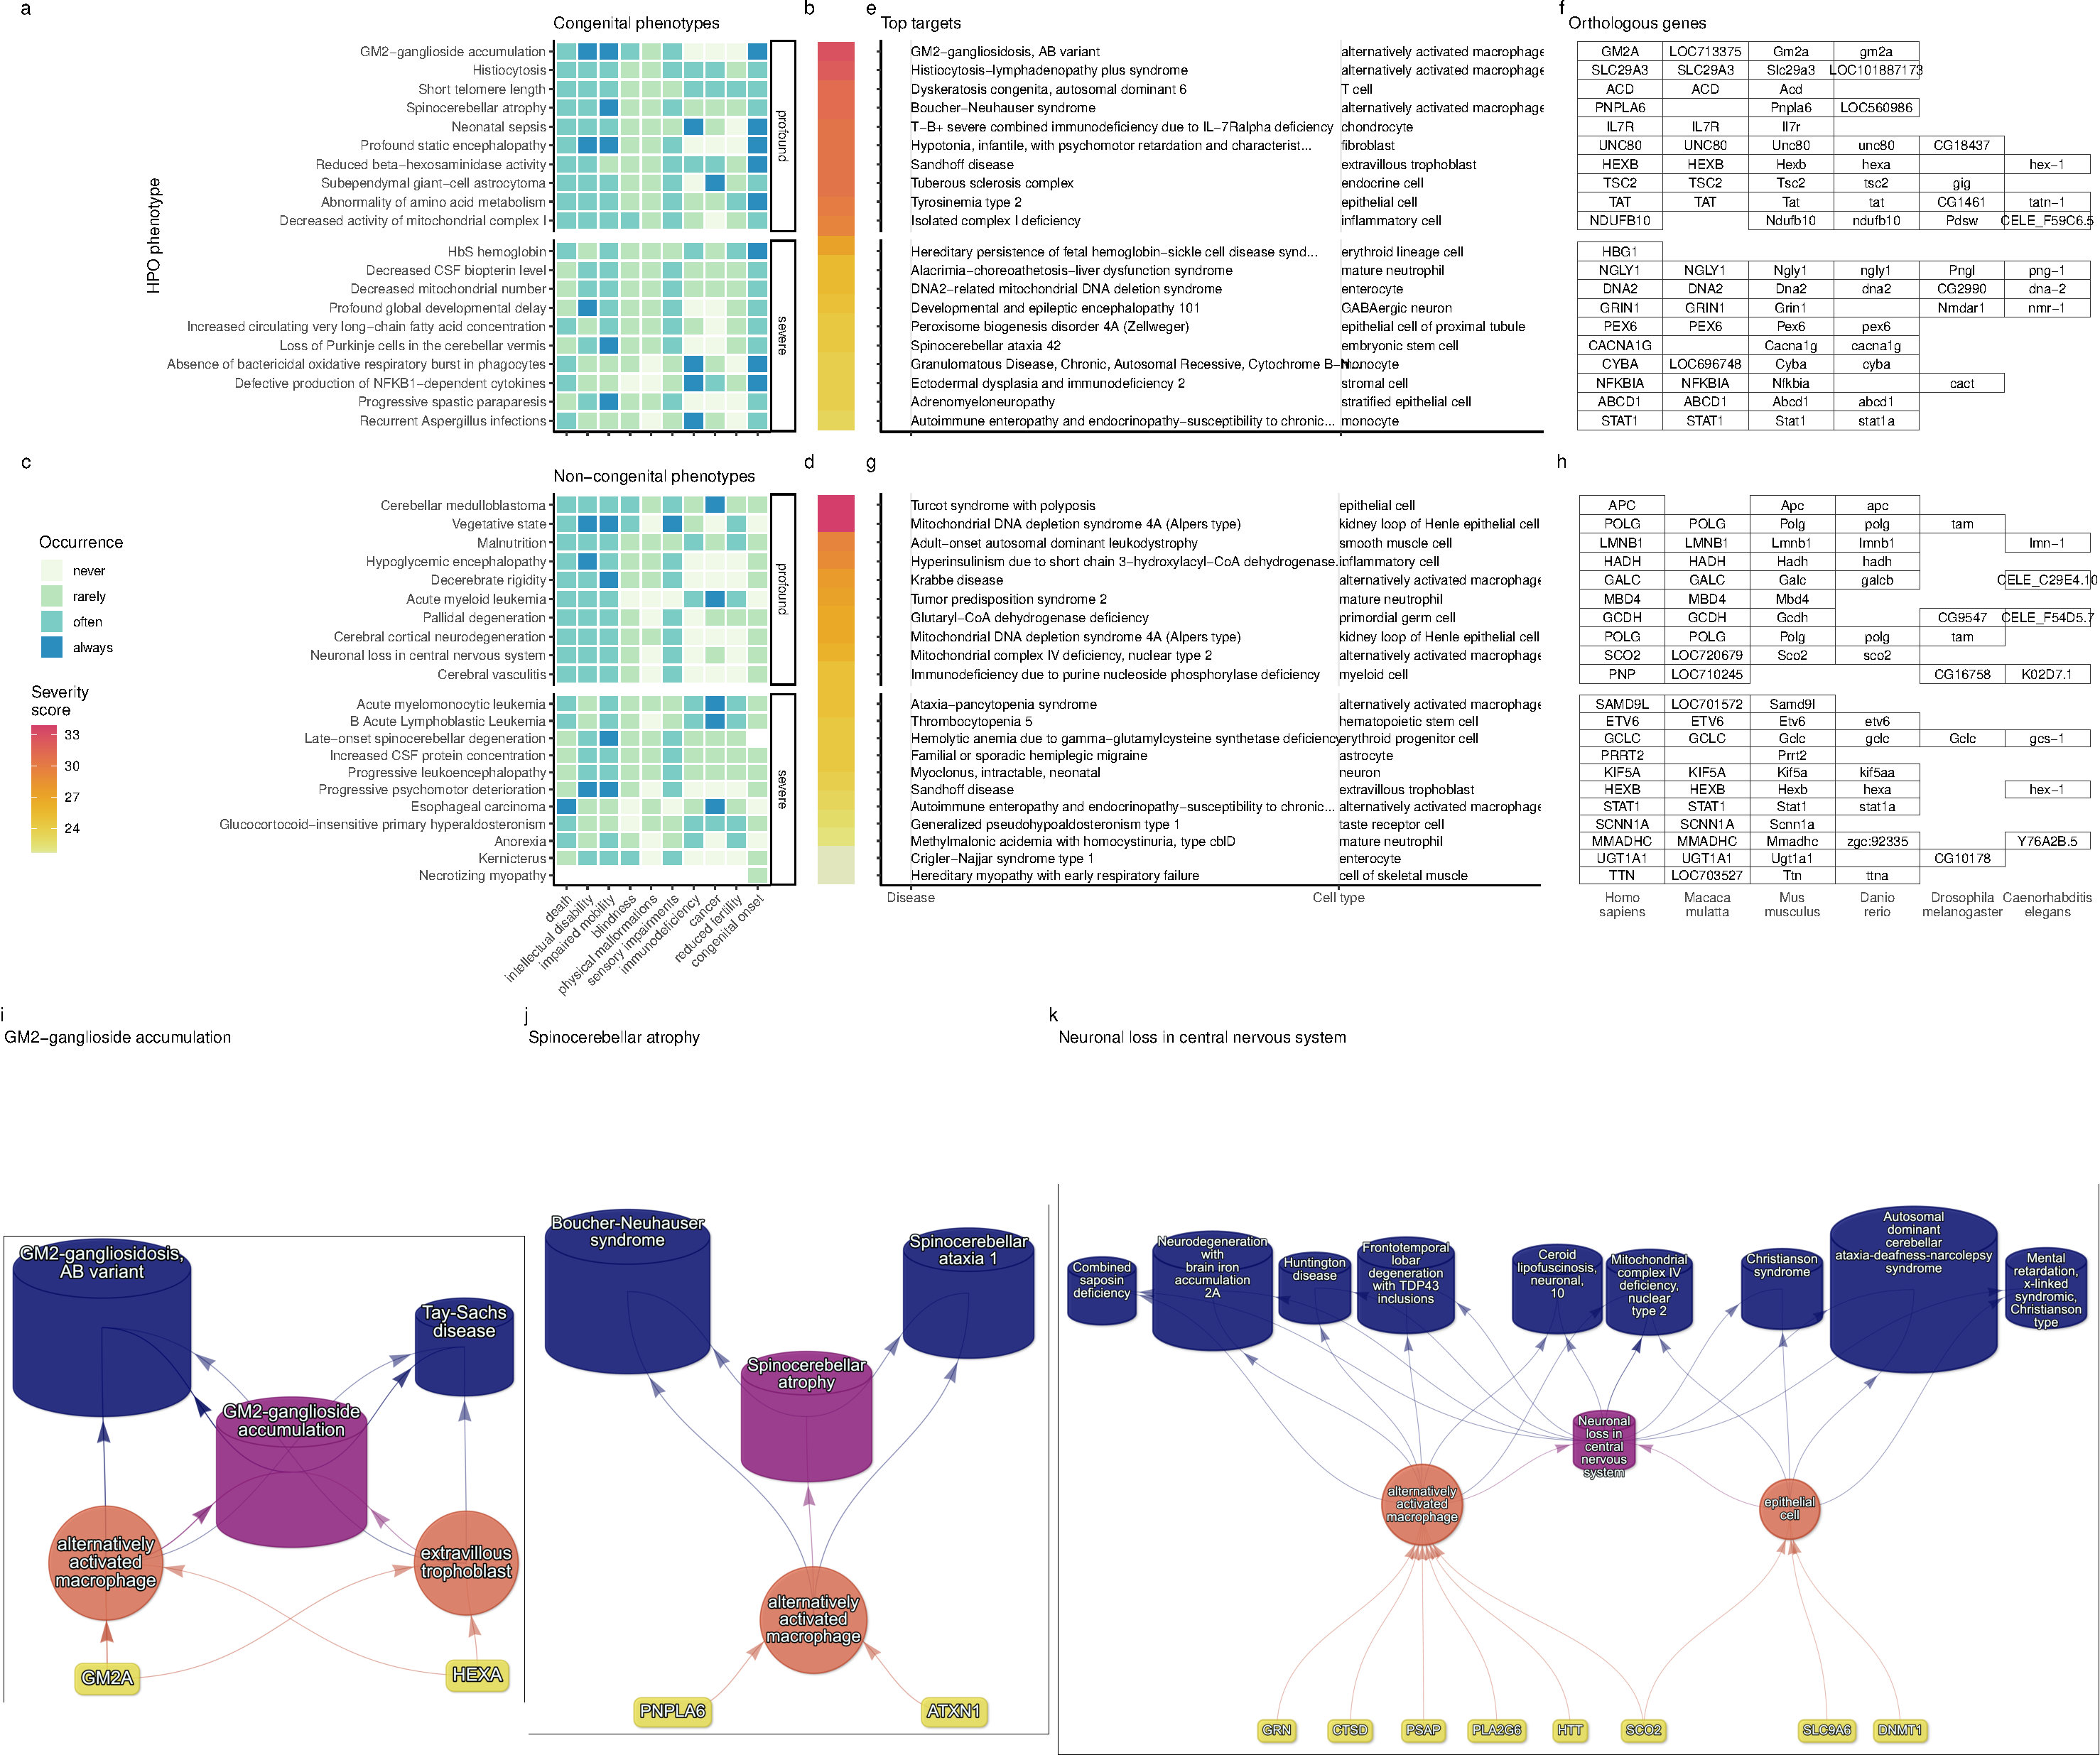
\includegraphics{index_files/figure-pdf/fig-therapy-examples-1.pdf}

}

\caption{\label{fig-therapy-examplesD08295A6-16DC-499D-85A8-8BA656E013A2}Top
40 prioritised gene therapy targets at multiple biological scales,
stratified by congenital (top row) vs.~non-congential phenotypes (bottom
row) as well as severity class (``profound'' or ``severe''). In this
plot, only the top 10 most severe phenotypes within a given
strata/substrata are shown \textbf{a,c}, Severity annotation generated
by GPT-4. \textbf{b,d}, Composite severity scores computed across all
severity metrics. \textbf{e,g}, Top mediator disease and cell
type-specific target for each phenotype. \textbf{f,h} top target gene
for each phenotype within humans (\emph{Homo sapiens}). We also include
the 1:1 ortholog of each human gene in several commonly used animal
models, including monkey (\emph{Macaca mulatta}), mouse (\emph{Mus
musculus}), zebrafish (\emph{Danio rerio}), fly (\emph{Drosophila
melanogaster}) and nematode (\emph{Caenorhabditis elegans}). Boxes are
empty where no 1:1 ortholog is known. \textbf{i-k} Example cell
type-specific gene therapy targets for several severe phenotypes and
their associated diseases. Each disease (blue cylinders) is connected to
its phenotype (purple cylinders) based on well-established clinical
observations recorded within the HPO\textsuperscript{11}. Phenotypes are
connected to cell types (red circles) via association testing between
weighted gene sets (FDR\textless0.05). Each cell type is connected to
the prioritised gene targets (yellow boxes) based on the driver gene
analysis.The thickness of the edges connecting the nodes represent the
(mean) fold-change from the bootstrapped enrichment tests. Nodes were
spatially arranged using the Sugiyama algorithm\textsuperscript{50}.}

\end{figure}%

From our prioritised targets, we selected the following four sets of
phenotypes or diseases as examples: `GM2-ganglioside accumulation',
`Spinocerebellar atrophy', `Neuronal loss in central nervous system'.
Only phenotypes with a GPT severity score greater than \(15\) were
considered to avoid overplotting and to focus on the more clinically
relevant phenotypes.

Tay-Sachs disease (TSD) is a devastating hereditary condition in which
children are born appearing healthy, which gradually degrades leading to
death after 3-5 years. The underlying cause is the toxic accumulation of
gangliosides in the nervous system due to a loss of the enzyme produced
by \emph{HEXA}. While this could in theory be corrected with gene
editing technologies, there remain some outstanding challenges. One of
which is identifying which cell types should be targeted to ensure the
most effective treatments. Here we identified alternatively activated
macrophages as the cell type most strongly associated with
`GM2-ganglioside accumulation'. The role of aberrant macrophage activity
in the regulation of ganglioside levels is supported by observation that
gangliosides accumulate within macrophages in TSD\textsuperscript{52},
as well as experimental evidence in rodent
models\textsuperscript{53.,54,55}. Our results not only corroborate
these findings, but propose macrophages as the primary causal cell type
in TSD, making it the most promising cell type to target in therapies.

Another challenge in TSD is early detection and diagnosis, before
irreversible damage has occurred. Our pipeline implicated extravillous
trophoblasts of the placenta in `GM2-ganglioside accumulation'. While
not necessarily a target for gene therapy, checking these cells \emph{in
utero} for an absence of \emph{HEXA} may serve as a viable biomarker as
these cells normally express the gene at high levels. Early detection of
TSD may lengthen the window of opportunity for therapeutic
intervention\textsuperscript{56}, especially when genetic sequencing is
not available or variants of unknown significance are found within
\emph{HEXA}\textsuperscript{57}.

Spinocerebellar atrophy is a debilitating and lethal phenotype that
occurs in diseases such as Spinocerebellar ataxia and Boucher-Nenhauser
syndrome. These diseases are characterised by progressive degeneration
of the cerebellum and spinal cord, leading to severe motor and cognitive
impairments. Our pipeline identified M2 macrophages as the only causal
cell type associated with `Spinocerebellar atrophy'. This strongly
suggests that degeneration of cerebellar Purkinje cells are in fact
downstream consequences of macrophage dysfunction, rather than being the
primary cause themselves. This is consistent with the known role of
macrophages, especially microglia, in neuroinflammation and other
neurodegenerative conditions such as Alzheimer's and Parkinsons'
disease\textsuperscript{58--60}. While experimental and postmortem
observational studies have implicated microglia in spinocerebellar
atrophy previously\textsuperscript{58}, our results provide a
statistically-supported and unbiased genetic link between known risk
genes and this cell type. Therefore, targeting M2 microglia in the
treatment of spinocerebellar atrophy may therefore represent a promising
therapeutic strategy. This is aided by the fact that there are mouse
models that perturb the ortholog of human spinocerebellar atrophy risk
genes
(e.g.~\href{https://www.informatics.jax.org/marker/MGI:104783}{\emph{Atxn1}},
\href{https://www.informatics.jax.org/marker/MGI:1354723}{\emph{Pnpla6}})
and reliably recapitulate the effects of this diseases at the cellular
(e.g.~loss of Purkinje cells), morphological (e.g.~atrophy of the
cerebellum, spinal cord, and muscles), and functional (e.g.~ataxia)
levels.

Next, we investigated the phenotype `Neuronal loss in the central
nervous system'. Despite the fact that this is a fairly broad phenotype,
we found that it was only significantly associated with 3 cell types
(alternatively activated macrophage, macrophage, epithelial cell),
specifically M2 macrophages and sinusoidal endothelial cells.

Skeletal dysplasia is a heterogeneous group of over 450 disorders that
affect the growth and development of bone and cartilage. This phenotype
can be lethal when deficient bone growth leads to the constriction of
vital organs such as the lungs. Even after surgical interventions, these
complications continue to arise as the child develops. Pharmacological
interventions to treat this condition have largely been ineffective.
While there are various cell types involved in skeletal system
development, our pipeline nominated chondrocytes as the causal cell type
underlying the lethal form of this condition
(Fig.~\ref{fig-therapy-examples-supp}). Assuringly, we found that the
disease `Achondrogenesis Type 1B' is caused by the genes \emph{SLC26A2}
and \emph{COL2A1} via chondrocytes. We also found that `Platyspondylic
lethal skeletal dysplasia, Torrance type'. Thus, in cases where surgical
intervention is insufficient, targeting these genes within chondrocytes
may prove a viable long-term solution for children suffering from lethal
skeletal dysplasia.

Alzheimer's disease (AD) is the most common neurodegenerative condition.
It is characterised by a set of variably penetrant phenotypes including
memory loss, cognitive decline, and cerebral proteinopathy.
Interestingly, we found that different forms of early onset AD (which
are defined by the presence of a specific disease gene) are each
associated with different cell types via different phenotypes
(Fig.~\ref{fig-therapy-examples-supp}). For example, AD 3 and AD 4 are
primarily associated with cells of the digestive system (`enterocyte',
`gastric goblet cell') and are implied to be responsible for the
phenotypes `Senile plaques', `Alzheimer disease', `Parietal
hypometabolism in FDG PET'. Meanwhile, AD 2 is primarily associated with
immune cells (`alternatively activated macrophage') and is implied to be
responsible for the phenotypes `Neurofibrillary tangles', `Long-tract
signs'. This suggests that different forms of AD may be driven by
different cell types and phenotypes, which may help to explain its
variability in onset and clinical presentation.

Finally, Parkinson's disease (PD) is characterised by motor symptoms
such as tremor, rigidity, and bradykinesia. However there are a number
of additional phenotypes associated with the disease that span multiple
physiological systems. PD 19a and PD 8 seemed to align most closely with
the canonical understanding of PD as a disease of the central nervous
system in that they implicated oligodendrocytes and neurons
(Fig.~\ref{fig-therapy-examples-supp}). Though the reference datasets
being used in this study were not annotated at sufficient resolution to
distinguish between different subtypes of neurons, in particular
dopaminergic neurons. PD 19a/8 also suggested that risk variants in
\emph{LRRK2} mediate their effects on PD through both myeloid cells and
oligodendrocytes by causing gliosis of the substantia nigra. The
remaining clusters of PD mechanisms revolved around chondrocytes (PD
20), amacrine cells of the eye (hereditary late-onset PD), and the
respiratory/immune system (PD 14). While the diversity in cell
type-specific mechanisms is somewhat surprising, it may help to explain
the wide variety of cross-system phenotypes frequently observed in PD.

It should be noted that the HPO only includes gene annotations for the
monogenic forms of AD and PD. However it has previously been shown that
there is at least partial overlap in their phenotypic and genetic
aetiology with respect to their common forms. Thus understanding the
monogenic forms of these diseases may shed light onto their more common
counterparts.

\subsection{Experimental model
translatability}\label{experimental-model-translatability}

We computed interspecies translatability scores using a combination of
both ontological (\(SIM_{o}\)) and genotypic (\(SIM_{g}\)) similarity
relative to each homologous human phenotype and its associated genes
\textbf{?@fig-animal-models}. In total, we mapped 278 non-human
phenotypes (in \emph{Caenorhabditis elegans}, \emph{Danio rerio},
\emph{Mus musculus}, \emph{Rattus norvegicus}) to 849 homologous human
phenotypes. Amongst the 5,252 phenotype within our prioritised therapy
targets, 354 had viable animal models in at least on non-human species.
Per species, the number of homologous phenotypes was: \emph{Danio rerio}
(n=214)\emph{Mus musculus} (n=150)\emph{Caenorhabditis elegans}
(n=35)\emph{Rattus norvegicus} (n=3). Amongst our prioritised targets
with a GPT-4 severity score of \textgreater10, the phenotypes with the
greatest animal model similarity were `Anterior vertebral fusion'
(\(SIM_{o,g}=0.97\)), `Disc-like vertebral bodies' (\(SIM_{o,g}=0.96\)),
`Metaphyseal enchondromatosis' (\(SIM_{o,g}=0.95\)), `Peripheral retinal
avascularization' (\(SIM_{o,g}=0.94\)), `Retinal vascular malformation'
(\(SIM_{o,g}=0.94\)).

\section{Discussion}\label{sec-discussion}

Across the 201 cell types and 11,047 RD-associated phenotypes
investigated, more than 46,514 significant phenotype-cell type
relationships were discovered. This presents a wealth of opportunities
to trace the mechanisms of rare diseases through multiple biological
scales. This in turn enhances our ability to study and treat causal
factors in disease with deeper understanding and greater precision.
These results recapitulate well-known relationships, while providing
additional cellular context to many of these known relationships, and
discovering novel relationships.

From our target prioritisation pipeline results, we highlight cell
type-specific mechanisms for `GM2-ganglioside accumulation' in Tay-Sachs
disease, spinocerebellar atrophy in spinocerebellar ataxia, and
`Neuronal loss in central nervous system' in a variety of diseases
(\textbf{?@fig-therapy-examples}). Of interest, all three of these
neurodegenerative phenotypes involved alternatively activated (M2)
macrophages. The role of macrophages in neurodegeneration is complex,
with both neuroprotective and neurotoxic functions, including the
clearance of misfolded proteins, the regulation of the blood-brain
barrier, and the modulation of the immune response\textsuperscript{61}.
We also recapitulated prior evidence that microglia, the resident
macrophages of the nervous system, are causally implicated in
Alzheimer's disease (AD)
(Fig.~\ref{fig-therapy-examples-supp})\textsuperscript{62}. An important
contribution of our current study is that we were able to pinpoint the
specific phenotypes of AD caused by macrophages to neurofibrillary
tangles and long-tract signs (reflexes that indicate the functioning of
spinal long fiber tracts). Other AD-associated phenotypes were caused by
other cell types (e.g.~gastric goblet cells, enterocytes).

Investigating RDs at the level of phenotypes offers several key
advantages. First, the vast majority of RDs only have one associated
gene (7,671/8,631 diseases = 89\%). Aggregating gene sets across
diseases into phenotype-centric ``buckets'' permits sufficiently
well-powered analyses, with an average of \textasciitilde{}\(76\) genes
per phenotype (median=7) \textbf{?@fig-diagram}. Second, we hypothesise
that these phenotype-level gene sets converge on a limited number of
molecular and cellular pathways. Perturbations to these pathways
manifest as one or more phenotypes which, when considered together, tend
to be clinically diagnosed as a certain disease. Third, RDs are often
highly heterogeneous in their clinical presentation across individuals,
leading to the creation of an ever increasing number of disease subtypes
(some of which only have a single documented case). In contrast, a
phenotype-centric approach enables us to more accurately describe a
particular individual's version of a disease without relying on the
generation of additional disease subcategories. By characterising an
individual's precise phenotypes over time, we may better understand the
underlying biological mechanisms that have caused their condition.
However, in order to achieve a truly precision-based approach to
clinical care, we must first characterise the molecular and cellular
mechanisms that cause the emergence of each phenotype. Here, we provide
a highly reproducible framework that enables this at the scale of the
entire phenome. This presents an opportunity to design basket trials of
patients with different diseases but overlapping phenotypes and cellular
mechanisms\textsuperscript{63}. It may be especially helpful for complex
patients with diagnostically ambiguous sets of phenotypes who would
otherwise be excluded from traditional clinical
trials\textsuperscript{64}.

It was paramount to the success of this study to ensure our results were
anchored in ground-truth benchmarks, generated falsifiable hypotheses,
and rigorously guarded against false-positive associations. Extensive
validation using multiple approaches demonstrated that our methodology
consistently recapitulates expected phenotype-cell type associations
(\textbf{?@fig-summary}-\textbf{?@fig-congenital}). This was made
possible by the existence of comprehensive, structured ontologies for
all phenotypes (HPO) and cell types (CL), which provide an abundance of
clear and falsifiable hypotheses for which to test our predictions
against. Several key examples include 1) strong enrichment of
associations between cell types and phenotypes within the same
anatomical systems (\textbf{?@fig-summary}b-d), 2) a strong relationship
between phenotype-specificity and the strength and number of cell type
associations (\textbf{?@fig-ontology-lvl}), 3) identification of the
precise cell subtypes involved in susceptibility to various subtypes of
recurrent bacterial infections (\textbf{?@fig-rni}), 4) a strong
positive correlation between the frequency of congenital onset of a
phenotype and the proportion of developmental cell types associated with
it (\textbf{?@fig-congenital})), and 5) consistent phenotype-cell type
associations across multiple independent single-cell datasets
(\textbf{?@fig-ctd-correlation}). Having validated our phenotype-cell
type associations, we then went on to demonstrate how these results may
be used in therapeutics development (\textbf{?@fig-therapy-examples}).

Diagnosis is an essential but challenging step in RD patient care.
Additional phenotypes that emerge over time may assist a clinician to
reach a more confident disease diagnosis. However many of these
phenotypes can have a serious impact on patient quality of life or
survival and avoiding them would be far better for patient outcomes.
Often times phenotypes alone cannot clearly pinpoint the disease and
thus a diagnosis is never reached. Having a more complete understanding
of the mechanisms underlying observed phenotypes allows clinicians to
far more effectively make predictions about what additional, less
obvious phenotypes they should search for to confirm or reject their
hypothesis of disease diagnosis (e.g.~with imaging or biomarker tests).

Unfortunately, there are currently only treatments available for less
than 5\% of RDs\textsuperscript{6}. Novel technologies including CRISPR,
prime editing, antisense oligonucleotides, viral vectors, and/or lipid
nanoparticles, have been undergone significant advances in the last
several years\textsuperscript{65--69} and proven remarkable clinical
success in an increasing number of clinical
applications\textsuperscript{70--73}. The U.S. Food and Drug
Administration (FDA) recently announced an landmark program aimed
towards improving the international regulatory framework to take
advantage of the evolving gene/cell therapy
technologies\textsuperscript{74} with the aim of bringing dozens more
therapies to patients in a substantially shorter timeframe than
traditional pharmaceutical product development (typically 5-20 years
with a median of 8.3 years)\textsuperscript{75}. While these
technologies have the potential to revolutionise RD medicine, their
successful application is dependent on first understanding the
mechanisms causing each disease.

To address this critical gap in knowledge, we used our results to create
a reproducible and customisable pipeline to nominate cell type-resolved
therapeutic targets
(\textbf{?@fig-therapy-filter}-\textbf{?@fig-therapy-examples}).
Targeting cell type-specific mechanisms underlying granular RD
phenotypes can improve therapeutic effectiveness by treating the causal
root of an individual's conditions\textsuperscript{66,76}. A cell
type-specific approach also helps to reduce the number of harmful side
effects caused by unintentionally delivering the therapeutic to
off-target tissues/cell types (which may induce aberrant gene activity),
especially when combined with technologies that can target cell surface
antigens (e.g viral vectors)\textsuperscript{77}. This has the
additional benefit of reducing the minimal effective dose of a
therapeutic, which can be both immunogenic and extremely financially
costly\textsuperscript{9,10,65,68}. Here, we demonstrate the utility of
a high-throughput evidence-based approach to RD therapeutics discovery
by highlighting several of the most promising therapeutic candidates.
Our pipeline takes into account a myriad of factors, including the
strength of the phenotype-cell type associations, symptom-cell type
associations, cell type-specificity of causal genes, the severity and
frequency of the phenotypes, suitability for gene therapy delivery
systems (e.g.~recombinant adeno-associated viral vectors (rAAV)), as
well as a quantitative analysis of phenotypic and genetic animal model
translatability (\textbf{?@fig-animal-models}). We validated these
candidates by comparing the proportional overlap with gene therapies
that are presently in the market or undergoing clinical trials, in which
we recovered \(81\)\% of all active gene therapies and
\(NaN \times 10^{-Inf}\)\% of failed gene therapies
(\textbf{?@fig-therapy-validate}, \textbf{?@fig-therapy-validate-all}).
Despite nominating a large number of putative targets, hypergeometric
tests confirmed that our targets were strongly enriched for targets of
existing therapies that are either approved or currently undergoing
clinical trials.

It should be noted that our study has several key limitations. First,
while our cell type datasets are amongst the most comprehensive human
scRNA-seq references currently available, they are nevertheless missing
certain tissues, cell types (e.g.~spermatocytes, oocytes), and life
stages (post-natal childhood, senility). It is also possible that we
have not captured certain cell state signatures that only occur in
disease (e.g.~disease-associated microglia\textsuperscript{78,79}).
Though we reasoned that using only control cell type signatures would
mitigate bias towards any particular disease, and avoid degradation of
gene signatures due to loss of function mutations. Second, the
collective knowledge of gene-phenotype and gene-disease associations is
far from complete and we fully anticipate that these annotations will
continue to expand and change well into the future. It is for this
reason we designed this study to be easily reproduced within a single
containerised script so that we (or others) may rerun it with updated
datasets at any point. Finally, causality is notoriously difficult to
prove definitively from associative testing alone, and our study is not
exempt from this rule. Despite this, there are several reasons to
believe that our approach is able to better approximate causal
relationships than traditional approaches. First, we did not
intentionally preselect any subset of phenotypes or cell types to
investigate here. Along with a scaling prestep during linear modelling,
this means that all the results are internally consistent and can be
directly compared to one another (in stark contrast to literature
meta-analyses). Furthermore, for the phenotype gene signatures we used
expert-curated GenCC annotations\textsuperscript{80,81} to weight the
current strength of evidence supporting a causal relationship between
each gene and phenotype. This is especially important for phenotypes
with large genes lists (thousands of annotations) for which some of the
relationships may be tenuous. Within the cell type references, we
deliberately chose to use specificity scores (rather than raw gene
expression) as this normalisation procedure has previously been
demonstrated to better distinguish between signatures of highly similar
cell types/subtypes\textsuperscript{82}.

Common ontology-controlled frameworks like the HPO open a wealth of new
opportunities, especially when addressing RDs. Services such as the
Matchmaker Exchange\textsuperscript{83,84} have enabled the discovery of
hundreds of underlying genetic etiologies, and led to the diagnosis of
many patients. This also opens the possibility of gathering cohorts of
geographically dispersed patients to run clinical trials, the only
viable option for treatment in many individuals. To further increase the
number of individuals who qualify for these treatments, as well as the
trial sample size, proposals have been made deviate from the traditional
single-disease clinical trial model and instead perform basket trials on
groups of RDs with shared molecular etiologies
(SaME)\textsuperscript{63}.

Moving forward, we are now actively seeking industry and academic
partnerships to begin experimentally validating our multi-scale target
predictions and exploring their potential for therapeutic translation.
Nevertheless, there are more promising therapeutic targets here than our
research group could ever hope to pursue by ourselves. In the interest
of accelerating research and ensuring RD patients are able to benefit
from this work as quickly as possible, we have decided to publicly
release all of the results described in this study. These can be
accessed in multiple ways, including through a suite of R packages as
well as a web app, the
\href{https://neurogenomics.github.io/rare_disease_celltyping_apps/home/}{Rare
Disease Celltyping Portal}. The latter allows our results to be easily
queried, filtered, visualised, and downloaded without any knowledge of
programming. Through these resources we aim to make our findings useful
to a wide variety of RD stakeholders including subdomain experts,
clinicians, advocacy groups, and patients.

\section{Conclusions}\label{sec-conclusions}

Ultimately, our primary objective was to develop a methodology capable
of generating high-throughput phenome-wide predictions while preserving
the accuracy and clinical utility typically associated with more
narrowly focused studies. With the rapid advancement of gene therapy
technologies, and a regulatory landscape that is evolving to better meet
the needs of a large and diverse patient population, there is finally
momentum to begin to realise the promise of personalised medicine. This
has especially important implications for the global RD community which
has remained relatively neglected. Here, we lay out the groundwork
necessary for this watershed moment by providing a scalable,
cost-effective, and fully reproducible means of resolving the
multi-scale, cell-type specific mechanisms of virtually all rare
diseases.

\section{Methods}\label{sec-methods}

\subsection{Human Phenotype Ontology}\label{human-phenotype-ontology}

The latest version of the HPO (release releases) was downloaded from the
EMBL-EBI Ontology Lookup Service\textsuperscript{85} and imported into R
using the \texttt{HPOExplorer} package. This R object was used to
extract ontological relationships between phenotypes as well as to
assign absolute and relative ontological levels to each phenotype. The
latest version of the HPO phenotype-to-gene mappings and phenotype
annotations were downloaded from the official HPO GitHub repository and
imported into R using \texttt{HPOExplorer}. This contains lists of genes
associated with phenotypes via particular diseases, formatted as three
columns in a table (gene, phenotype, disease).

However, not all genes have equally strong evidence of causality with a
disease or phenotype, especially when considering that the variety of
resources used to generate these annotations (OMIM, Orphanet, DECIPHER)
use variable methodologies (e.g.~expert-curated review of the medical
literature vs.~automated text mining of the literature). Therefore we
imported data from the Gene Curation Coalition
(GenCC)\textsuperscript{80,81}, which (as of 2024-05-17) 22,060 evidence
scores across 7,259 diseases and 5,165 genes. Evidence scores are
defined by GenCC using a standardised ordinal rubric which we then
encoded as a semi-quantitative score ranging from 0 (no evidence of
disease-gene relationship) to 6 (strongest evidence of disease-gene
relationship) (see \textbf{?@tbl-gencc}). As each Disease-Gene pair can
have multiple entries (from different studies) with different levels of
evidence, we then summed evidence scores per Disease-Gene pair to
generate aggregated Disease-by-Gene evidence scores. This procedure can
be described as follows.

Let us denote:

\begin{itemize}
\item
  \(D\) as diseases.
\item
  \(P\) as phenotypes in the HPO.
\item
  \(G\) as genes
\item
  \(S\) as the evidence scores describing the strength of the
  relationship between each Disease-Gene pair.
\item
  \(M_{ij}\) as the aggregated Disease-by-Gene evidence score matrix.
\end{itemize}

\[
M_{ij} = \sum_{k=1}^{\text{f}} D_i G_j S_k
\]

Next, we extracted Disease-Gene-Phenotype relationships from the
annotations file distributed by the HPO
(\emph{phenotype\_to\_genes.txt}). This provides a list of genes
associated with phenotypes via particular diseases, but does not include
any strength of evidence scores.

Here we define: - \(A_{ijk}\) as the Disease-Gene-Phenotype
relationships. - \(D_i\) as the \(i\)th disease. - \(G_j\) as the
\(j\)th gene. - \(P_k\) as the \(k\)th phenotype.

\[
A_{ijk} = D_i G_j P_k
\]

In order to assign evidence scores to each Phenotype-Gene relationship,
we combined the aforementioned datasets from GenCC (\(M_{ij}\)) and HPO
(\(A_{ijk}\)) by merging on the gene and disease ID columns. For each
phenotype, we then computed the mean of Disease-Gene scores across all
diseases for which that phenotype is a symptom. This resulted in a final
2D tensor of Phenotype-by-Gene evidence scores (\(L_{ij}\)):

\hfill\break
\hfill\break

$$
 \eqnmarkbox[NavyBlue]{n1}{ L_{ij} } = 
 \begin{cases}
  \frac{\sum_{k=1}^{\text{f}} 
    \eqnmarkbox[Cerulean]{n3a}{D_i G_j} 
    \eqnmarkbox[BlueViolet]{n5}{P_k} 
    }{\text{f}}, 
  \text{if } \eqnmarkbox[Cerulean]{n3b}{D_i G_j} 
    \in \eqnmarkbox[blue]{n4a}{A},
  \\
  1, \hspace{2.2cm}
  \text{if } \eqnmarkbox[Cerulean]{n3c}{D_i G_j} 
    \notin\eqnmarkbox[blue]{n4b}{A}
 \end{cases}
$$
\annotate[yshift=1em]{left}{n1}{Tensor of Phenotype-by-Gene \\evidence scores}
\annotate[yshift=2.5em]{right}{n3a,n3b,n3c}{Tensor of Disease-by-Gene \\evidence scores}
\annotate[yshift=-2.5em]{below,left}{n4a,n4b}{Disease-by-Gene-by-Phenotype \\relationships}
\annotate[yshift=1em, xshift=-1em]{right}{n5}{Phenotype}

\hfill\break

Construction of the tensor of Phenotype-by-Gene evidence scores.

\hfill\break

Histograms of evidence score distributions at each step in processing
can be found in \textbf{?@fig-evidence-histograms}.

\subsection{Single-cell transcriptomic
atlases}\label{single-cell-transcriptomic-atlases}

In this study, the gene by cell type specificity matrix was constructed
using the Descartes Human transcriptome atlas of foetal gene expression,
which contains a mixture of single-nucleus and single-cell RNA-seq data
(collected with sci-RNA-seq3)\textsuperscript{28}. This dataset contains
377,456 cells representing 77 distinct cell types across 15 tissues. All
121 human foetal samples ranged from 72 to 129 days in estimated
postconceptual age. To independently replicate our findings, we also
used the Human Cell Landscape which contains single-cell transcriptomic
data (collected with microwell-seq) from embryonic, foetal, and adult
human samples across 49 tissues\textsuperscript{29}.

Specificity matrices were generated separately for each transcriptomic
atlas using the R package \texttt{EWCE} (v1.11.3)\textsuperscript{82}.
Within each atlas, cell types were defined using the authors' original
freeform annotations in order to preserve the granularity of cell
subtypes as well as incorporate expert-identified rare cell types. Cell
types were only aligned and aggregated to the level of corresponding
Cell Ontology (CL)\textsuperscript{34} annotations afterwards when
generating summary figures and performing cross-atlas analyses. Using
the original gene-by-cell count matrices from each single-cell atlas, we
computed gene-by-cell type expression specificity matrices as follows.
Genes with very no expression across any cell types were considered to
be uninformative and were therefore removed from the input gene-by-cell
matrix \(F(g,i,c)\).

Next, we calculated the mean expression per cell type and normalised the
resulting matrix to transform it into a gene-by-cell type expression
specificity matrix (\(S_{g,c}\)). In other words, each gene in each cell
type had a 0-1 score where 1 indicated the gene was mostly specifically
expressed in that particular cell type relative to all other cell types.
This procedure was repeated separately for each of the single-cell
atlases and can be summarised as:

\hfill\break

\begin{equation*}
  \eqnmarkbox[orange]{s1}{S_{gc}}
  =
  \frac{
    \eqnmarkbox[purple]{s3a}{
      \frac{
        \sum_{i=1}^{|L|} F_{gic}
      }{
        N_c  
      }
    } 
  }{
   \eqnmarkbox[OrangeRed]{s6}{\sum_{r=1}^{k}}(
     \eqnmarkbox[purple]{s3b}{
      \frac{
        \sum_{i=1}^{|L|} F_{gic}
      }{
        N_c  
      }
    } 
   ) 
  }
\end{equation*}
\annotate[yshift=1em]{left}{s1}{Gene-by-cell type specificity matrix} 
\annotate[yshift=2em]{left}{s3a,s3b}{Compute mean expression of each gene per cell type} 
\annotate{below,left}{s6}{Compute row sums of \\mean gene-by-cell type matrix}

\hfill\break

\subsection{Phenotype-cell type
associations}\label{phenotype-cell-type-associations-1}

To test for relationships between each pairwise combination of phenotype
(n=11,047) and cell type (n=201) we ran a series of univariate
generalised linear models implemented via the \texttt{stats::glm}
function in R. First, we filtered the gene-by-phenotype evidence score
matrix (\(L_{ij}\)) and the gene-by-cell type expression specificity
matrix (\(S_{gc}\)) to only include genes present in both matrices
(n=4,949 genes in the Descartes Human analyses; n=4,653 genes in the
Human Cell Landscape analyses). Then, within each matrix any rows or
columns with a sum of 0 were removed as these were uninformative data
points that did not vary. To improve interpretability of the results
\(\beta\) coefficient estimates across models (i.e.~effect size), we
performed a scaling prestep on all dependent and independent variables.
Initial tests showed that this had virtually no impact on the total
number of significant results or any of the benchmarking metrics based
on p-value thresholds \textbf{?@fig-summary}. This scaling prestep
improved our ability to rank cell types by the strength of their
association with a given phenotype as determined by separate linear
models.

We repeated the aforementioned procedure separately for each of the
single-cell references. Once all results were generated using both cell
type references (2,206,994 association tests total), we applied
Benjamini-Hochberg false discovery rate\textsuperscript{86} (denoted as
\(FDR_{pc}\)) to account for multiple testing. Of note, we applied this
correction across all results at once (as opposed to each single-cell
reference separately) to ensure the \(FDR_{pc}\) was stringently
controlled for across all tests performed in this study.

\subsection{Symptom-cell type
associations}\label{symptom-cell-type-associations}

Here we define a symptom as a phenotype as it presents within the
context of the specific disease. The features of a given symptom can be
described as the subset of genes annotated to phenotype \(p\) via a
particular disease \(d\), denoted as \(G_{dp}\)
(\textbf{?@fig-diagram}). To attribute our phenotype-level cell type
enrichment signatures to specific diseases, we first identified the gene
subset that was most strongly driving the phenotype-cell type
association by computing the intersect of genes that were both in the
phenotype annotation and within the top 25\% specificity percentile for
the associated cell type. We then computed the intersect between symptom
genes (\(G_{dp}\)) and driver genes (\(G_{pc}\)), resulting in the gene
subset \(G_{d \cap p \cap c}\). Only \(G_{d \cap p \cap c}\) gene sets
with 25\% or greater overlap with the symptom gene subset (\(G_{dp}\))
were kept. This procedure was repeated for all phenotype-cell
type-disease triads, which can be summarised as follows:

\hfill\break

\begin{equation*}
  \frac{
     \eqnmarkbox[Chartreuse3]{g1}{|G_{d \cap p \cap c} |}
    }{
       \eqnmarkbox[Emerald]{g2}{|G_{dp}|}} 
  \geq \eqnmarkbox[SeaGreen]{g3}{.25} 
\end{equation*}
\annotate[yshift=1em]{left}{g1}{Intersect between \\symptom genes ($G_{dp}$) and driver genes ($G_{pc}$)} 
\annotate[yshift=-1em]{below,left}{g2}{Symptom genes \\(i.e. genes annotated to a phenotype\\ via a specific disease)} 
\annotate[yshift=-1em]{below,right}{g3}{Minimum proportion of overlap \\between $G_{dpc}$ and $G_{dp}$}

\hfill\break
\hfill\break

\subsection{Validation of expected phenotype-cell type
relationships}\label{validation-of-expected-phenotype-cell-type-relationships-1}

We first sought to confirm that our tests (across both single-cell
references) were able to recover expected phenotype-cell type
relationships across seven high-level branches within the HPO
(\textbf{?@fig-summary}), including abnormalities of the cardiovascular
system, endocrine system, eye, immune system, musculoskeletal system,
nervous system, and respiratory system. Within each branch the number of
significant tests in a given cell type were plotted
(\textbf{?@fig-summary}b). Mappings between freeform annotations (the
level at which we performed our phenotype- cell type association tests)
provided by the original atlas authors and their closest CL term
equivalents were provided by CellxGene\textsuperscript{26}. CL terms
along the \emph{x-axis} of \textbf{?@fig-summary}b were assigned colours
corresponding to which HPO branch showed the greatest number of
enrichments (after normalising within each branch to account for
differences in scale). The normalised colouring allows readers to
quickly assess which HPO branch was most often associated with each cell
type, while accounting for differences in the number of phenotypes
across branches. We then ran a series of Analysis of Variance (ANOVA)
tests to determine whether (within a given branch) a given cell type was
more often enriched (FDR\textless0.05) within that branch relative to
all of the other HPO branches of an equivalent level in the ontology
(including all branches not shown in \textbf{?@fig-summary}b). After
applying Benjamini-Hochberg multiple testing
correction\textsuperscript{86} (denoted as \(FDR _{b,c}\)), we annotated
each respective branch-by-cell type bar according to the significance
(**** : \(FDR _{b,c}<1e-04\), *** : \(FDR _{b,c}<0.001\), ** :
\(FDR _{b,c}<0.01\), * : \(FDR _{b,c}<0.05\)). Cell types in
\textbf{?@fig-summary}a-b were ordered along the \emph{x-axis} according
to a dendrogram derived from the CL ontology (\textbf{?@fig-summary}c),
which provides ground-truth semantic relationships between all cell
types (e.g.~different neuronal subtypes are grouped together).

As an additional measure of the accuracy of our phenotype-cell types
test results we identified conceptually matched branches across the HPO
and the CL (\textbf{?@fig-summary}d and \textbf{?@tbl-celltypes}). For
example, `Abnormality of the cardiovascular system' in the HPO was
matched with `cardiocytes' in the CL which includes all cell types
specific to the heart. Analogously, `Abnormality of the nervous system'
in the HPO was matched with `neural cell' in the CL which includes all
descendant subtypes of neurons and glia. This cross-ontology matching
was repeated for each HPO branch and can be referred to as on-target
cell types. Within each branch, the \(-log_{10}(FDR _{pc})\) values of
on-target cell types were binned by rounding to the nearest integer
(\emph{x-axis}) and the percentage of tests for on-target cell types
relative to all cell types were computed at each bin (\emph{y-axis})
(\textbf{?@fig-summary}d). The baseline level (dotted horizontal line)
illustrates the percentage of on-target cell types relative to the total
number of observed cell types. Any percentages above this baseline level
represent greater than chance representation of the on-target cell types
in the significant tests.

\subsection{Monarch Knowledge Graph
recall}\label{monarch-knowledge-graph-recall-1}

Finally, we gathered known phenotype-cell type relationships from the
Monarch Knowledge Graph (MKG), a comprehensive database of links between
many aspects of disease biology\textsuperscript{87}. This currently
includes 103 links between HPO phenotypes (n=103) and CL cell types
(n=79). Of these, we only considered the 82 phenotypes that we were able
to test given that our ability to generate associations was dependent on
the existence of gene annotations within the HPO. We considered
instances where we found a significant relationship between exactly
matching pairs of HPO-CL terms as a hit.

However, as the cell types in MKG were not necessarily annotated at the
same level as our single-cell references, we considered instances where
the MKG cell type was an ancestor term of our cell type (e.g.~`myeloid
cell' vs.~`monocyte'), or \emph{vice versa}, as hits. We also adjusted
ontological distance by computing the ratio between the observed
ontological distance and the smallest possible ontological distance for
that cell type given the cell type that were available in our references
(\(dist_{adjusted}=(\frac{dist_{observed}+1}{dist_{minimum}+1})-1\)).
This provides a way of accurately measuring how dissimilar our
identified cell types were for each phenotype-cell type association
(\textbf{?@fig-monarch-recall}).

\subsection{Annotation of phenotypes using generative large language
models}\label{annotation-of-phenotypes-using-generative-large-language-models-1}

Only a small fraction of the the phenotypes in HPO (\textless1\%) have
metadata annotations containing information on their time course,
consequences, and severity. This is due to the time-consuming nature of
manually annotating thousands of phenotypes. To generate such
annotations at scale, we previously used Generative Pre-trained
Transformer 4 (GPT-4), a large language model (LLM) as implemented
within OpenAI's Application Programming Interface
(API)\textsuperscript{32}. After extensive prompt engineering and
ground-truth benchmarking, we were able to acquire annotations on how
often each phenotype directly causes intellectual disability, death,
impaired mobility, physical malformations, blindness, sensory
impairments, immunodeficiency, cancer, reduced fertility, or is
associated with a congenital onset. These criteria were previously
defined in surveys of medical experts as a means of systematically
assessing phenotype severity\textsuperscript{88}. Responses for each
metric were provided in a consistent one-word format which could be one
of: `never', `rarely', `often', `always'. This procedure was repeated in
batches (to avoid exceeding token limits) until annotations were
gathered for 16,982/18,082 HPO phenotypes.

We then encoded these responses into a semi-quantitative scoring system
(`never'=0, `rarely'=1, `often'=2, `always'=3), which were then weighted
by multiplying a semi-subjective scoring of the relevance of each metric
to the concept of severity on a scale from \(1.0\)-\(6.0\), with \(6.0\)
being the most severe (`death'=6, `intellectual\_disability'=5,
`impaired\_mobility'=4, `physical\_malformations'=3, `blindness'=4,
`sensory\_impairments'=3, `immunodeficiency'=3, `cancer'=3,
`reduced\_fertility'=1, `congenital\_onset'=1). Finally, the product of
the score was normalised to a quantitative severity score ranging from
0-100, where 100 is the theoretical maximum severity score. This
phenotype severity scoring procedure can be expressed as follows.

Let us denote:

\begin{itemize}
\item
  \(p\) : a phenotype in the HPO.
\item
  \(j\) : the identity of a given annotation metric (i.e.~clinical
  characteristic, such as `intellectual disability' or `congenital
  onset').
\item
  \(W_j\): the assigned weight of metric \(j\).
\item
  \(F_j\): the maximum possible value for metric \(j\) (equivalent
  across all \(j\)).
\item
  \(F_{pj}\) : the numerically encoded value of annotation metric \(j\)
  for phenotype \(p\).
\item
  \(NSS_p\): the final composite severity score for phenotype \(p\)
  after applying normalisation to align values to a 0-100 scale and
  ensure equivalent meaning regardless of which other phenotypes are
  being analysed in addition to \(p\). This allows for direct
  comparability of severity scores across studies with different sets of
  phenotypes.
\end{itemize}

\hfill\break
\hfill\break

\begin{equation*}
  \eqnmarkbox[Brown4]{nss}{NSS_p}
  =
  \frac{ 
    \eqnmarkbox[Goldenrod]{nss2}{\sum_{j=1}^{m}} 
    (
      \eqnmarkbox[Goldenrod4]{nss3}{F_{pj}}
      \times 
      \eqnmarkbox[IndianRed4]{nss4}{W_j}
    )
    }{
    \eqnmarkbox[Tan]{nss5}{\sum_{j=1}^{m}(\max\{F_j\} \times W_j)} 
  } \times 100
\end{equation*}
\annotate[yshift=1em]{left}{nss}{Normalised Severity Score \\for each phenotype}
\annotate[yshift=3em]{left}{nss2}{Sum of weighted annotation values \\across all metrics}
\annotate[yshift=3em]{right}{nss3}{Numerically encoded annotation value \\of metric $j$ for phenotype $p$}
\annotate[yshift=1em]{right}{nss4}{Weight for metric $j$} 
\annotate[yshift=-1em]{below,right}{nss5}{Theoretical maximum severity score}

\hfill\break

\subsection{Congenital phenotypes are associated with foetal cell
types}\label{congenital-phenotypes-are-associated-with-foetal-cell-types-1}

The GPT-4 annotations also enabled us to assess whether foetal cell
types were more often significantly associated with congenital
phenotypes in our Human Cell Landscape results as this single-cell
reference contained both adult and foetal versions of cell types
(\textbf{?@fig-congenital}). To do this, we performed a chi-squared
(\(\chi^2\)) test on the proportion of significantly associated cell
types containing any of the substrings `fetal', `fetus', `primordial',
`hESC' or `embryonic' (within cell types annotations from the original
Human Cell Landscape authors\textsuperscript{29}) vs.~those associated
without, stratified by how often the corresponding phenotype had a
congenital onset according to the GPT phenotype annotations (including
`never', `rarely', `often', `always'). In addition, a series of
\(\chi^2\) tests were performed within each congenital onset frequency
strata, to determine whether the observed proportion of foetal cell
types vs.~non-foetal cell types significantly deviated from the
proportions expected by chance.

We next tested whether the proportion of tests with significant
associations with foetal cell types varied across the major HPO branches
using a \(\chi^2\) test. We also performed separate \(\chi^2\) test
within each branch to determine whether the proportion of significant
associations with foetal cell types was significantly different from
chance.

\subsection{Therapeutic target
identification}\label{therapeutic-target-identification-1}

We developed a systematic and automated strategy for identifying
putative cell type-specific gene targets for each phenotype based on a
series of filters at phenotype, cell type, and gene levels. The entire
target prioritisation procedure can be replicated with a single
function: \texttt{MSTExplorer::prioritise\_targets}. This function
automates all of the reference data gathering (e.g.~phenotype metadata,
cell type metadata, cell type signature reference, gene lengths,
severity tiers) and takes a variety of arguments at each step for
greater customisability. Each step is described in detail in
\textbf{?@tbl-filters}. Phenotypes that often or always caused physical
malformations (according to the GPT-4 annotations) were also removed
from the final prioritised targets list, as these were unlikely to be
amenable to gene therapy interventions. Finally, phenotypes were sorted
by their composite severity scores such that the most severe phenotypes
were ranked the highest.

\subsection{Therapeutic target
validation}\label{therapeutic-target-validation-1}

To assess whether our prioritised therapeutic targets were likely to be
viable, we computed the overlap between our gene targets and those of
existing gene therapies at various stages of clinical development
(\textbf{?@fig-therapy-validate}). Gene targets were obtained for each
therapy from the Therapeutic Target Database (TTD; release 2024-07-23)
and mapped onto standardised HUGO Gene Nomenclature Committee (HGNC)
gene symbols using the \texttt{orthogene} R package. We stratified our
overlap metrics according to whether the therapies had failed
(unsuccessful clinical trials or withdrawn), or were non-failed
(successful or ongoing clinical trials). We then conducted
hypergeometric tests to determine whether the observed overlap between
our prioritised targets and the non-failed therapy targets was
significantly greater than expected by chance (i.e.~enrichment). We also
conducted a second hypergeometric test to determine whether the observed
overlap between our prioritised targets and the failed therapy targets
was significantly less than expected by chance (i.e.~depletion).
Finally, we repeated the analysis against all therapeutic targets, not
just those of gene therapies, to determine whether our prioritised
targets had relevance to other therapeutic modalities.

\subsection{Experimental model
translatability}\label{experimental-model-translatability-1}

To improve the likelihood of successful translation between preclinical
animal models and human patients, we created an interspecies
translatability prediction tool for each phenotype nominated by our gene
therapy prioritised pipeline (\textbf{?@fig-animal-models}). First, we
extracted ontological similarity scores of homologous phenotypes across
species from the MKG\textsuperscript{87}. Briefly, the ontological
similarity scores (\(SIM_o\)) are computed for each homologous pair of
phenotypes across two ontologies by calculating the overlap in
homologous phenotypes that are ancestors or descendants of the target
phenotype. Next, we generated genotypic similarity scores (\(SIM_g\))
for each homologous phenotype pair by computing the proportion of 1:1
orthologous genes using gene annotation from their respective
ontologies. Interspecies orthologs were also obtained from the MKG.
Finally, both scores are multiplied together to yield a unified
ontological-genotypic similarity score (\(SIM_{o,g}\)).

\subsection{Novel R packages}\label{novel-r-packages}

To facilitate all analyses described in this study and to make them more
easily reproducible by others, we created several open-source R
packages.
\href{https://github.com/neurogenomics/KGExplorer}{\texttt{KGExplorer}}
imports and analyses large-scale biomedical knowledge graphs and
ontologies.
\href{https://github.com/neurogenomics/HPOExplorer}{\texttt{HPOExplorer}}
aids in managing and querying the directed acyclic ontology graph within
the HPO.
\href{https://github.com/neurogenomics/MSTExplorer}{\texttt{MSTExplorer}}
facilitates the efficient analysis of many thousands of phenotype-cell
type association tests, and provides a suite of multi-scale therapeutic
target prioritisation and visualisation functions. These R packages also
include various functions for distributing the post-processed results
from this study in an organised, tabular format. Of note,
\texttt{MSTExplorer::load\_example\_results} loads all summary
statistics from our phenotype-cell type tests performed here.

\subsection{Rare Disease Celltyping
Portal}\label{rare-disease-celltyping-portal}

To further increase the ease of access for stakeholders in the RD
community without the need for programmatic experience, we developed a
series of web apps to interactively explore, visualise, and download the
results from our study. Collectively, these web apps are called the Rare
Disease Celltyping Portal. The landing page for the website was made
using HTML, CSS, and javascript and the web apps were created using the
Shiny Web application framework for R and deployed on the shinyapps.io
server. The website can be accessed at
\url{https://neurogenomics.github.io/rare_disease_celltyping_apps/home}.
All code used to generate the website can be found at
\url{https://github.com/neurogenomics/rare_disease_celltyping_apps}.

\newpage{}

\section{Tables}\label{tables}

\begin{longtable}[]{@{}
  >{\raggedright\arraybackslash}p{(\columnwidth - 6\tabcolsep) * \real{0.4359}}
  >{\raggedright\arraybackslash}p{(\columnwidth - 6\tabcolsep) * \real{0.1923}}
  >{\raggedright\arraybackslash}p{(\columnwidth - 6\tabcolsep) * \real{0.2436}}
  >{\raggedright\arraybackslash}p{(\columnwidth - 6\tabcolsep) * \real{0.1282}}@{}}
\toprule\noalign{}
\begin{minipage}[b]{\linewidth}\raggedright
\end{minipage} & \begin{minipage}[b]{\linewidth}\raggedright
DescartesHuman
\end{minipage} & \begin{minipage}[b]{\linewidth}\raggedright
HumanCellLandscape
\end{minipage} & \begin{minipage}[b]{\linewidth}\raggedright
all
\end{minipage} \\
\midrule\noalign{}
\endhead
\bottomrule\noalign{}
\endlastfoot
tests significant & 19,929 & 26,585 & 46,514 \\
tests & 848,078 & 1,358,916 & 2,206,994 \\
tests significant (\%) & 2.35 & 1.96 & 2.11 \\
cell types significant & 77 & 124 & 201 \\
cell types & 77 & 124 & 201 \\
cell types significant (\%) & 100 & 100 & 100 \\
phenotypes significant & 7,340 & 9,049 & 9,575 \\
phenotypes tested & 11,014 & 10,959 & 11,028 \\
phenotypes & 11,047 & 11,047 & 11,047 \\
phenotypes significant (\%) & 66.4 & 81.9 & 86.7 \\
diseases significant & 8,628 & 8,627 & 8,628 \\
diseases & 8,631 & 8,631 & 8,631 \\
diseases significant (\%) & 100 & 100 & 100 \\
cell types per phenotype (mean) & 1.81 & 2.43 & 4.22 \\
cell types per phenotype (median) & 1 & 2 & 3 \\
cell types per phenotype (min) & 0 & 0 & 0 \\
cell types per phenotype (max) & 31 & 28 & 59 \\
phenotypes per cell type (mean) & 259 & 214 & 231 \\
phenotypes per cell type (median) & 252 & 200 & 209 \\
phenotypes per cell type (min) & 71 & 57 & 57 \\
phenotypes per cell type (max) & 696 & 735 & 735 \\
\end{longtable}

\newpage{}

\begin{longtable}[]{@{}
  >{\raggedright\arraybackslash}p{(\columnwidth - 4\tabcolsep) * \real{0.0413}}
  >{\raggedright\arraybackslash}p{(\columnwidth - 4\tabcolsep) * \real{0.1446}}
  >{\raggedright\arraybackslash}p{(\columnwidth - 4\tabcolsep) * \real{0.8140}}@{}}
\toprule\noalign{}
\begin{minipage}[b]{\linewidth}\raggedright
level
\end{minipage} & \begin{minipage}[b]{\linewidth}\raggedright
step
\end{minipage} & \begin{minipage}[b]{\linewidth}\raggedright
description
\end{minipage} \\
\midrule\noalign{}
\endhead
\bottomrule\noalign{}
\endlastfoot
NA & 1. start & NA \\
Cell type & 2. q threshold & Keep only cell type-phenotype association
results at q\textless=0.05. \\
Phenotype & 3. keep descendants & Remove phenotypes belonging to a
certain branch of the HPO,as defined by an ancestor term. \\
Phenotype & 4. info content threshold & Keep only phenotypes with a
minimum information criterion score(computed from the HPO). \\
Phenotype & 5. severity threshold & Keep only phenotypes with mean
Severity equal to or below the threshold. \\
Symptom & 6. pheno frequency threshold & Keep only phenotypes with mean
frequency equal to or above the threshold(i.e.~how frequently a
phenotype is associated with any diseases inwhich it occurs). \\
Gene & 7. symptom gene overlap & Ensure that genes nominated at the
phenotype-level alsoappear in the genes overlapping at the cell
type-specific symptom-level. \\
Gene & 8. evidence score threshold & Remove genes that are below an
aggregate phenotype-gene evidence score threshold. \\
Gene & 9. add driver genes & Keep only genes that are driving the
association with a given phenotype(inferred by the intersection of
phenotype-associated genes and gene withhigh-specificity quantiles in
the target cell type). \\
Symptom & 10. symptom intersection threshold & Minimum proportion of
genes overlapping between a symptom gene list(phenotype-associated genes
in the context of a particular disease)and the phenotype-cell type
association driver genes. \\
Gene & 11. gene frequency threshold & Keep only genes at or above a
certain mean frequency threshold(i.e.~how frequently a gene is
associated with a given phenotypewhen observed within a disease). \\
Phenotype & 12. prune ancestors & Remove redundant ancestral phenotypes
when at least one of theirdescendants already exist. \\
All & 13. top n & Sort candidate targets by a preferred order of metrics
andonly return the top N targets per cell type-phenotype combination. \\
NA & 14. end & NA \\
\end{longtable}

\newpage{}

\section{Data Availability}\label{data-availability}

All data is publicly available through the following resources:

\begin{itemize}
\tightlist
\item
  Human Phenotype Ontology (\url{https://hpo.jax.org})
\item
  GenCC (\url{https://thegencc.org/})
\item
  Descartes Human scRNA-seq atlas
  (\url{https://cellxgene.cziscience.com/collections/c114c20f-1ef4-49a5-9c2e-d965787fb90c})
\item
  Human Cell Landscape scRNA-seq atlas
  (\url{https://cellxgene.cziscience.com/collections/38833785-fac5-48fd-944a-0f62a4c23ed1})
\item
  Processed Cell Type Datasets (\emph{ctd\_DescartesHuman.rds} and
  \emph{ctd\_HumanCellLandscape.rds};
  \url{https://github.com/neurogenomics/MSTExplorer/releases})
\item
  Gene x Phenotype association matrix (\emph{hpo\_matrix.rds};
  \url{https://github.com/neurogenomics/MSTExplorer/releases})
\item
  Rare Disease Celltyping Portal
  (\url{https://neurogenomics.github.io/rare_disease_celltyping_apps/home})
\end{itemize}

\section{Code Availability}\label{code-availability}

All code is made freely available through the following GitHub
repositories:

\begin{itemize}
\tightlist
\item
  \texttt{KGExplorer}
  (\url{https://github.com/neurogenomics/KGExplorer})
\item
  \texttt{HPOExplorer}
  (\url{https://github.com/neurogenomics/HPOExplorer})
\item
  \texttt{MSTExplorer}
  (\url{https://github.com/neurogenomics/MSTExplorer})
\item
  Code to replicate analyses
  (\url{https://github.com/neurogenomics/rare_disease_celltyping})
\item
  Cell type-specific gene target prioritisation
  (\url{https://neurogenomics.github.io/RareDiseasePrioritisation/reports/prioritise_targets})
\item
  Complement system gene list
  (\url{https://www.genenames.org/data/genegroup/\#!/group/492})
\end{itemize}

\section{Acknowledgements}\label{acknowledgements}

We would like to thank the following individuals for their insightful
feedback and assistance with data resources: Sarah J. Marzi, Gerton
Lunter, Peter Robinson, Melissa Haendel, Ben Coleman, Nico Matentzoglu,
Shawn T. O'Neil, Alan E. Murphy, Sarada Gurung.

\subsection{Funding}\label{funding}

This work was supported by a UK Dementia Research Institute (UK DRI)
Future Leaders Fellowship {[}MR/T04327X/1{]} and the UK DRI which
receives its funding from UK DRI Ltd, funded by the UK Medical Research
Council, Alzheimer's Society and Alzheimer's Research UK.

\section*{References}\label{references}
\addcontentsline{toc}{section}{References}

\phantomsection\label{refs}
\begin{CSLReferences}{0}{0}
\bibitem[\citeproctext]{ref-Ferreira2019-jp}
\CSLLeftMargin{1. }%
\CSLRightInline{Ferreira, C. R. The burden of rare diseases. \emph{Am.
J. Med. Genet. A} \textbf{179}, 885--892 (2019).}

\bibitem[\citeproctext]{ref-Zhu2020-vo}
\CSLLeftMargin{2. }%
\CSLRightInline{Zhu, Q. \emph{et al.} An integrative knowledge graph for
rare diseases, derived from the genetic and rare diseases information
center ({GARD}). \emph{J. Biomed. Semantics} \textbf{11}, 13 (2020).}

\bibitem[\citeproctext]{ref-noauthor_undated-kp}
\CSLLeftMargin{3. }%
\CSLRightInline{Rare diseases {BioResource}.}

\bibitem[\citeproctext]{ref-Marwaha2022-uy}
\CSLLeftMargin{4. }%
\CSLRightInline{Marwaha, S., Knowles, J. W. \& Ashley, E. A. A guide for
the diagnosis of rare and undiagnosed disease: Beyond the exome.
\emph{Genome Med.} \textbf{14}, 23 (2022).}

\bibitem[\citeproctext]{ref-Molster2016-da}
\CSLLeftMargin{5. }%
\CSLRightInline{Molster, C. \emph{et al.} Survey of healthcare
experiences of australian adults living with rare diseases.
\emph{Orphanet J. Rare Dis.} \textbf{11}, 30 (2016).}

\bibitem[\citeproctext]{ref-Halley2022-pd}
\CSLLeftMargin{6. }%
\CSLRightInline{Halley, M. C., Smith, H. S., Ashley, E. A., Goldenberg,
A. J. \& Tabor, H. K. A call for an integrated approach to improve
efficiency, equity and sustainability in rare disease research in the
united states. \emph{Nat. Genet.} \textbf{54}, 219--222 (2022).}

\bibitem[\citeproctext]{ref-Institute_of_Medicine_US_Committee_on_Accelerating_Rare_Diseases_Research_and_Orphan_Product_Development2010-vj}
\CSLLeftMargin{7. }%
\CSLRightInline{Institute of Medicine (US) Committee on Accelerating
Rare Diseases Research and Orphan Product Development, Field, M. J. \&
Boat, T. F. \emph{Coverage and Reimbursement: Incentives and
Disincentives for Product Development}. (National Academies Press (US),
2010).}

\bibitem[\citeproctext]{ref-Yates2022-ra}
\CSLLeftMargin{8. }%
\CSLRightInline{Yates, N. \& Hinkel, J. The economics of moonshots:
Value in rare disease drug development. \emph{Clin. Transl. Sci.}
\textbf{15}, 809--812 (2022).}

\bibitem[\citeproctext]{ref-Nuijten2022-yc}
\CSLLeftMargin{9. }%
\CSLRightInline{Nuijten, M. Pricing zolgensma - the world's most
expensive drug. \emph{J Mark Access Health Policy} \textbf{10}, 2022353
(2022).}

\bibitem[\citeproctext]{ref-Thielen2022-ud}
\CSLLeftMargin{10. }%
\CSLRightInline{Thielen, F. W., Heine, R. J. S. D., Berg, S. van den,
Ham, R. M. T. T. \& Groot, C. A. U. Towards sustainability and
affordability of expensive cell and gene therapies? Applying a
cost-based pricing model to estimate prices for libmeldy and zolgensma.
\emph{Cytotherapy} \textbf{24}, 1245--1258 (2022).}

\bibitem[\citeproctext]{ref-Gargano2024-fc}
\CSLLeftMargin{11. }%
\CSLRightInline{Gargano, M. A. \emph{et al.} The human phenotype
ontology in 2024: Phenotypes around the world. \emph{Nucleic Acids Res.}
\textbf{52}, D1333--D1346 (2024).}

\bibitem[\citeproctext]{ref-Kohler2019-pc}
\CSLLeftMargin{12. }%
\CSLRightInline{Köhler, S. \emph{et al.} Expansion of the human
phenotype ontology ({HPO}) knowledge base and resources. \emph{Nucleic
Acids Res.} \textbf{47}, D1018--D1027 (2019).}

\bibitem[\citeproctext]{ref-Kohler2021-wk}
\CSLLeftMargin{13. }%
\CSLRightInline{Köhler, S. \emph{et al.} The human phenotype ontology in
2021. \emph{Nucleic Acids Res.} \textbf{49}, D1207--D1217 (2021).}

\bibitem[\citeproctext]{ref-Robinson2008-ys}
\CSLLeftMargin{14. }%
\CSLRightInline{Robinson, P. N. \emph{et al.} The human phenotype
ontology: A tool for annotating and analyzing human hereditary disease.
\emph{Am. J. Hum. Genet.} \textbf{83}, 610--615 (2008).}

\bibitem[\citeproctext]{ref-Nguengang_Wakap2020-cz}
\CSLLeftMargin{15. }%
\CSLRightInline{Nguengang Wakap, S. \emph{et al.} Estimating cumulative
point prevalence of rare diseases: Analysis of the orphanet database.
\emph{Eur. J. Hum. Genet.} \textbf{28}, 165--173 (2020).}

\bibitem[\citeproctext]{ref-noauthor_2022-ok}
\CSLLeftMargin{16. }%
\CSLRightInline{Rare diseases, common challenges. \emph{Nat. Genet.}
\textbf{54}, 215 (2022).}

\bibitem[\citeproctext]{ref-Amberger2019-vl}
\CSLLeftMargin{17. }%
\CSLRightInline{Amberger, J. S., Bocchini, C. A., Scott, A. F. \&
Hamosh, A. {OMIM.org}: Leveraging knowledge across phenotype-gene
relationships. \emph{Nucleic Acids Res.} \textbf{47}, D1038--D1043
(2019).}

\bibitem[\citeproctext]{ref-Amberger2017-tg}
\CSLLeftMargin{18. }%
\CSLRightInline{Amberger, J. S. \& Hamosh, A. Searching online mendelian
inheritance in man ({OMIM)}: A knowledgebase of human genes and genetic
phenotypes. \emph{Curr. Protoc. Bioinformatics} \textbf{58},
1.2.1--1.2.12 (2017).}

\bibitem[\citeproctext]{ref-McKusick2007-di}
\CSLLeftMargin{19. }%
\CSLRightInline{McKusick, V. A. Mendelian inheritance in man and its
online version, {OMIM}. \emph{Am. J. Hum. Genet.} \textbf{80}, 588--604
(2007).}

\bibitem[\citeproctext]{ref-Maiella2013-oo}
\CSLLeftMargin{20. }%
\CSLRightInline{Maiella, S., Rath, A., Angin, C., Mousson, F. \& Kremp,
O. {[}Orphanet and its consortium: Where to find expert-validated
information on rare diseases{]}. \emph{Rev. Neurol.} \textbf{169 Suppl
1}, S3--8 (2013).}

\bibitem[\citeproctext]{ref-Weinreich2008-wm}
\CSLLeftMargin{21. }%
\CSLRightInline{Weinreich, S. S., Mangon, R., Sikkens, J. J., Teeuw, M.
E. en \& Cornel, M. C. {[}Orphanet: A european database for rare
diseases{]}. \emph{Ned. Tijdschr. Geneeskd.} \textbf{152}, 518--519
(2008).}

\bibitem[\citeproctext]{ref-Firth2009-qg}
\CSLLeftMargin{22. }%
\CSLRightInline{Firth, H. V. \emph{et al.} {DECIPHER}: Database of
chromosomal imbalance and phenotype in humans using ensembl resources.
\emph{Am. J. Hum. Genet.} \textbf{84}, 524--533 (2009).}

\bibitem[\citeproctext]{ref-Baysoy2023-vt}
\CSLLeftMargin{23. }%
\CSLRightInline{Baysoy, A., Bai, Z., Satija, R. \& Fan, R. The
technological landscape and applications of single-cell multi-omics.
\emph{Nat. Rev. Mol. Cell Biol.} \textbf{24}, 695--713 (2023).}

\bibitem[\citeproctext]{ref-Haque2017-bn}
\CSLLeftMargin{24. }%
\CSLRightInline{Haque, A., Engel, J., Teichmann, S. A. \& Lönnberg, T. A
practical guide to single-cell {RNA-sequencing} for biomedical research
and clinical applications. \emph{Genome Med.} \textbf{9}, 75 (2017).}

\bibitem[\citeproctext]{ref-Qi2023-ev}
\CSLLeftMargin{25. }%
\CSLRightInline{Qi, R. \& Zou, Q. Trends and potential of machine
learning and deep learning in drug study at {Single-Cell} level.
\emph{Research} \textbf{6}, 0050 (2023).}

\bibitem[\citeproctext]{ref-CZI_Single-Cell_Biology_Program2023-fs}
\CSLLeftMargin{26. }%
\CSLRightInline{CZI Single-Cell Biology Program \emph{et al.} {CZ}
{CELL\(\times\)GENE} discover: A single-cell data platform for scalable
exploration, analysis and modeling of aggregated data. \emph{bioRxiv}
2023.10.30.563174 (2023).}

\bibitem[\citeproctext]{ref-Svensson2020-lg}
\CSLLeftMargin{27. }%
\CSLRightInline{Svensson, V., Veiga Beltrame, E. da \& Pachter, L. A
curated database reveals trends in single-cell transcriptomics.
\emph{Database} \textbf{2020}, (2020).}

\bibitem[\citeproctext]{ref-Cao2020-qz}
\CSLLeftMargin{28. }%
\CSLRightInline{Cao, J. \emph{et al.} A human cell atlas of fetal gene
expression. \emph{Science} \textbf{370}, (2020).}

\bibitem[\citeproctext]{ref-Han2020-iq}
\CSLLeftMargin{29. }%
\CSLRightInline{Han, X. \emph{et al.} Construction of a human cell
landscape at single-cell level. \emph{Nature} \textbf{581}, 303--309
(2020).}

\bibitem[\citeproctext]{ref-kawabataImprovingCellspecificRecombination2024}
\CSLLeftMargin{30. }%
\CSLRightInline{Kawabata, H. \emph{et al.}
\href{https://doi.org/10.1016/j.omtm.2024.101185}{Improving
cell-specific recombination using AAV vectors in the murine CNS by
capsid and expression cassette optimization}. \emph{Molecular Therapy
Methods \& Clinical Development} \textbf{32}, (2024).}

\bibitem[\citeproctext]{ref-ocarrollAAVTargetingGlial2021}
\CSLLeftMargin{31. }%
\CSLRightInline{O'Carroll, S. J., Cook, W. H. \& Young, D.
\href{https://doi.org/10.3389/fnmol.2020.618020}{AAV targeting of glial
cell types in the central and peripheral nervous system and relevance to
human gene therapy}. \emph{Frontiers in Molecular Neuroscience}
\textbf{13}, (2021).}

\bibitem[\citeproctext]{ref-murphyHarnessingGenerativeAI2024}
\CSLLeftMargin{32. }%
\CSLRightInline{Murphy, K., Schilder, B. M. \& Skene, N. G. Harnessing
generative AI to annotate the severity of all phenotypic abnormalities
within the Human Phenotype Ontology.
doi:\href{https://doi.org/10.1101/2024.06.10.24308475}{10.1101/2024.06.10.24308475}.}

\bibitem[\citeproctext]{ref-distefanoGeneCurationCoalition2022}
\CSLLeftMargin{33. }%
\CSLRightInline{DiStefano, M. T. \emph{et al.}
\href{https://doi.org/10.1016/j.gim.2022.04.017}{The gene curation
coalition: A global effort to harmonize gene--disease evidence
resources}. \emph{Genetics in Medicine} \textbf{24}, 1732--1742 (2022).}

\bibitem[\citeproctext]{ref-Diehl2016-gt}
\CSLLeftMargin{34. }%
\CSLRightInline{Diehl, A. D. \emph{et al.} The cell ontology 2016:
Enhanced content, modularization, and ontology interoperability.
\emph{J. Biomed. Semantics} \textbf{7}, 44 (2016).}

\bibitem[\citeproctext]{ref-Heim2014-du}
\CSLLeftMargin{35. }%
\CSLRightInline{Heim, C. E. \emph{et al.} Myeloid-derived suppressor
cells contribute to staphylococcus aureus orthopedic biofilm infection.
\emph{J. Immunol.} \textbf{192}, 3778--3792 (2014).}

\bibitem[\citeproctext]{ref-Pidwill2020-le}
\CSLLeftMargin{36. }%
\CSLRightInline{Pidwill, G. R., Gibson, J. F., Cole, J., Renshaw, S. A.
\& Foster, S. J. The role of macrophages in staphylococcus aureus
infection. \emph{Front. Immunol.} \textbf{11}, 620339 (2020).}

\bibitem[\citeproctext]{ref-Stoll2018-dc}
\CSLLeftMargin{37. }%
\CSLRightInline{Stoll, H. \emph{et al.} Staphylococcal enterotoxins
{Dose-Dependently} modulate the generation of {Myeloid-Derived}
suppressor cells. \emph{Front. Cell. Infect. Microbiol.} \textbf{8}, 321
(2018).}

\bibitem[\citeproctext]{ref-Tebartz2015-xs}
\CSLLeftMargin{38. }%
\CSLRightInline{Tebartz, C. \emph{et al.} A major role for
myeloid-derived suppressor cells and a minor role for regulatory {T}
cells in immunosuppression during staphylococcus aureus infection.
\emph{J. Immunol.} \textbf{194}, 1100--1111 (2015).}

\bibitem[\citeproctext]{ref-Zhou2016-kq}
\CSLLeftMargin{39. }%
\CSLRightInline{Zhou, Z., Xu, M.-J. \& Gao, B. Hepatocytes: A key cell
type for innate immunity. \emph{Cell. Mol. Immunol.} \textbf{13},
301--315 (2016).}

\bibitem[\citeproctext]{ref-Dixon2013-ok}
\CSLLeftMargin{40. }%
\CSLRightInline{Dixon, L. J., Barnes, M., Tang, H., Pritchard, M. T. \&
Nagy, L. E. Kupffer cells in the liver. \emph{Compr. Physiol.}
\textbf{3}, 785--797 (2013).}

\bibitem[\citeproctext]{ref-Ladhani2019-nf}
\CSLLeftMargin{41. }%
\CSLRightInline{Ladhani, S. N. \emph{et al.} Invasive meningococcal
disease in patients with complement deficiencies: A case series
(2008-2017). \emph{BMC Infect. Dis.} \textbf{19}, 522 (2019).}

\bibitem[\citeproctext]{ref-Rosain2017-ih}
\CSLLeftMargin{42. }%
\CSLRightInline{Rosain, J. \emph{et al.} Strains responsible for
invasive meningococcal disease in patients with terminal complement
pathway deficiencies. \emph{J. Infect. Dis.} \textbf{215}, 1331--1338
(2017).}

\bibitem[\citeproctext]{ref-The_International_Meningococcal_Genetics_Consortium2010-if}
\CSLLeftMargin{43. }%
\CSLRightInline{The International Meningococcal Genetics Consortium.
Genome-wide association study identifies variants in the {CFH} region
associated with host susceptibility to meningococcal disease.
\emph{Nature Genetics} \textbf{42}, 772--776 (2010).}

\bibitem[\citeproctext]{ref-Lung2019-il}
\CSLLeftMargin{44. }%
\CSLRightInline{Lung, T. \emph{et al.} The complement system in liver
diseases: Evidence-based approach and therapeutic options. \emph{J
Transl Autoimmun} \textbf{2}, 100017 (2019).}

\bibitem[\citeproctext]{ref-Reis2015-yz}
\CSLLeftMargin{45. }%
\CSLRightInline{Reis, E. S. \emph{et al.} Applying complement
therapeutics to rare diseases. \emph{Clin. Immunol.} \textbf{161},
225--240 (2015).}

\bibitem[\citeproctext]{ref-Seal2023-pa}
\CSLLeftMargin{46. }%
\CSLRightInline{Seal, R. L. \emph{et al.} Genenames.org: The {HGNC}
resources in 2023. \emph{Nucleic Acids Res.} \textbf{51}, D1003--D1009
(2023).}

\bibitem[\citeproctext]{ref-Al-Hamoudi2009-le}
\CSLLeftMargin{47. }%
\CSLRightInline{Al-Hamoudi, W. K. Severe autoimmune hepatitis triggered
by varicella zoster infection. \emph{World J. Gastroenterol.}
\textbf{15}, 1004--1006 (2009).}

\bibitem[\citeproctext]{ref-Brewer2018-dg}
\CSLLeftMargin{48. }%
\CSLRightInline{Brewer, E. C. \& Hunter, L. Acute liver failure due to
disseminated varicella zoster infection. \emph{Case Reports Hepatol}
\textbf{2018}, 1269340 (2018).}

\bibitem[\citeproctext]{ref-Eshchar1973-tz}
\CSLLeftMargin{49. }%
\CSLRightInline{Eshchar, J., Reif, L., Waron, M. \& Alkan, W. J. Hepatic
lesion in chickenpox. A case report. \emph{Gastroenterology}
\textbf{64}, 462--466 (1973).}

\bibitem[\citeproctext]{ref-Sugiyama1981-ev}
\CSLLeftMargin{50. }%
\CSLRightInline{Sugiyama, K., Tagawa, S. \& Toda, M. Methods for visual
understanding of hierarchical system structures. \emph{IEEE Trans. Syst.
Man Cybern.} \textbf{11}, 109--125 (1981).}

\bibitem[\citeproctext]{ref-Liu2011-qd}
\CSLLeftMargin{51. }%
\CSLRightInline{Liu, X. \emph{et al.} The therapeutic target database:
An internet resource for the primary targets of approved, clinical trial
and experimental drugs. \emph{Expert Opin. Ther. Targets} \textbf{15},
903--912 (2011).}

\bibitem[\citeproctext]{ref-fendersonChapterDevelopmentalGenetic2009}
\CSLLeftMargin{52. }%
\CSLRightInline{Fenderson, B. A. Chapter 6 - developmental and genetic
diseases. in \emph{Pathology secrets (third edition)} (ed. Damjanov, I.)
98--119 (Mosby, 2009).
doi:\href{https://doi.org/10.1016/B978-0-323-05594-9.00006-4}{10.1016/B978-0-323-05594-9.00006-4}.}

\bibitem[\citeproctext]{ref-vilcaesGangliosideSynthesisPlasma2020}
\CSLLeftMargin{53. }%
\CSLRightInline{Vilcaes, A. A., Garbarino-Pico, E., Torres Demichelis,
V. \& Daniotti, J. L.
\href{https://doi.org/10.3390/ijms21031063}{Ganglioside synthesis by
plasma membrane-associated sialyltransferase in macrophages}.
\emph{International Journal of Molecular Sciences} \textbf{21}, 1063
(2020).}

\bibitem[\citeproctext]{ref-yoheGangliosideAlterationsStimulated1985}
\CSLLeftMargin{54. }%
\CSLRightInline{Yohe, H. C., Coleman, D. L. \& Ryan, J. L.
\href{https://doi.org/10.1016/0005-2736(85)90141-5}{Ganglioside
alterations in stimulated murine macrophages}. \emph{Biochimica et
Biophysica Acta (BBA) - Biomembranes} \textbf{818}, 81--86 (1985).}

\bibitem[\citeproctext]{ref-demirGM2GangliosideAccumulation2020}
\CSLLeftMargin{55. }%
\CSLRightInline{Demir, S. A., Timur, Z. K., Ateş, N., Martínez, L. A. \&
Seyrantepe, V. \href{https://doi.org/10.1186/s12974-020-01947-6}{GM2
ganglioside accumulation causes neuroinflammation and behavioral
alterations in a mouse model of early onset tay-sachs disease}.
\emph{Journal of Neuroinflammation} \textbf{17}, 277 (2020).}

\bibitem[\citeproctext]{ref-solovyevaNewApproachesTaySachs2018}
\CSLLeftMargin{56. }%
\CSLRightInline{Solovyeva, V. V. \emph{et al.}
\href{https://doi.org/10.3389/fphys.2018.01663}{New approaches to
tay-sachs disease therapy}. \emph{Frontiers in Physiology} \textbf{9},
(2018).}

\bibitem[\citeproctext]{ref-hoffmanNextgenerationDNASequencing2013}
\CSLLeftMargin{57. }%
\CSLRightInline{Hoffman, J. D. \emph{et al.}
\href{https://doi.org/10.1002/mgg3.37}{Next-generation DNA sequencing of
HEXA: A step in the right direction for carrier screening}.
\emph{Molecular Genetics \& Genomic Medicine} \textbf{1}, 260--268
(2013).}

\bibitem[\citeproctext]{ref-ferroRoleMicrogliaAtaxias2019}
\CSLLeftMargin{58. }%
\CSLRightInline{Ferro, A., Sheeler, C., Rosa, J.-G. \& Cvetanovic, M.
\href{https://doi.org/10.1016/j.jmb.2019.01.016}{Role of microglia in
ataxias}. \emph{Journal of molecular biology} \textbf{431}, 1792--1804
(2019).}

\bibitem[\citeproctext]{ref-holMicroglialTranscriptomicsMeets2022}
\CSLLeftMargin{59. }%
\CSLRightInline{Hol, E. M. \& Pasterkamp, R. J. Microglial
transcriptomics meets genetics: New disease leads. \emph{Nature Reviews
Neurology} 1--2 (2022)
doi:\href{https://doi.org/10.1038/s41582-022-00633-w}{10.1038/s41582-022-00633-w}.}

\bibitem[\citeproctext]{ref-lopesAtlasGeneticEffects2020a}
\CSLLeftMargin{60. }%
\CSLRightInline{Lopes, K. de P. \emph{et al.} Atlas of genetic effects
in human microglia transcriptome across brain regions, aging and disease
pathologies. \emph{bioRxiv} 2020.10.27.356113 (2020)
doi:\href{https://doi.org/10.1101/2020.10.27.356113}{10.1101/2020.10.27.356113}.}

\bibitem[\citeproctext]{ref-gaoMicrogliaNeurodegenerativeDiseases2023}
\CSLLeftMargin{61. }%
\CSLRightInline{Gao, C., Jiang, J., Tan, Y. \& Chen, S.
\href{https://doi.org/10.1038/s41392-023-01588-0}{Microglia in
neurodegenerative diseases: mechanism and potential therapeutic
targets}. \emph{Signal Transduction and Targeted Therapy} \textbf{8},
1--37 (2023).}

\bibitem[\citeproctext]{ref-mcquadeMicrogliaAlzheimerDisease2019}
\CSLLeftMargin{62. }%
\CSLRightInline{Mcquade, A. \& Blurton-jones, M. Microglia in
alzheimer's disease : Exploring how genetics and phenotype influence
risk. \emph{Journal of Molecular Biology} 1--13 (2019)
doi:\href{https://doi.org/10.1016/j.jmb.2019.01.045}{10.1016/j.jmb.2019.01.045}.}

\bibitem[\citeproctext]{ref-Zanello2023-zd}
\CSLLeftMargin{63. }%
\CSLRightInline{Zanello, G. \emph{et al.} Targeting shared molecular
etiologies to accelerate drug development for rare diseases. \emph{EMBO
Mol. Med.} \textbf{15}, e17159 (2023).}

\bibitem[\citeproctext]{ref-Diaz-Santiago2020-ep}
\CSLLeftMargin{64. }%
\CSLRightInline{Dı́az-Santiago, E. \emph{et al.} Phenotype-genotype
comorbidity analysis of patients with rare disorders provides insight
into their pathological and molecular bases. \emph{PLoS Genet.}
\textbf{16}, e1009054 (2020).}

\bibitem[\citeproctext]{ref-Bueren2023-ma}
\CSLLeftMargin{65. }%
\CSLRightInline{Bueren, J. A. \& Auricchio, A. Advances and challenges
in the development of gene therapy medicinal products for rare diseases.
\emph{Hum. Gene Ther.} \textbf{34}, 763--775 (2023).}

\bibitem[\citeproctext]{ref-Bulaklak2020-ta}
\CSLLeftMargin{66. }%
\CSLRightInline{Bulaklak, K. \& Gersbach, C. A. The once and future gene
therapy. \emph{Nat. Commun.} \textbf{11}, 5820 (2020).}

\bibitem[\citeproctext]{ref-Godbout2023-uo}
\CSLLeftMargin{67. }%
\CSLRightInline{Godbout, K. \& Tremblay, J. P. Prime editing for human
gene therapy: Where are we now? \emph{Cells} \textbf{12}, (2023).}

\bibitem[\citeproctext]{ref-Kohn2023-vh}
\CSLLeftMargin{68. }%
\CSLRightInline{Kohn, D. B., Chen, Y. Y. \& Spencer, M. J. Successes and
challenges in clinical gene therapy. \emph{Gene Ther.} \textbf{30},
738--746 (2023).}

\bibitem[\citeproctext]{ref-Zhao2023-qy}
\CSLLeftMargin{69. }%
\CSLRightInline{Zhao, Z., Shang, P., Mohanraju, P. \& Geijsen, N. Prime
editing: Advances and therapeutic applications. \emph{Trends
Biotechnol.} \textbf{41}, 1000--1012 (2023).}

\bibitem[\citeproctext]{ref-Darrow2019-om}
\CSLLeftMargin{70. }%
\CSLRightInline{Darrow, J. J. Luxturna: {FDA} documents reveal the value
of a costly gene therapy. \emph{Drug Discov. Today} \textbf{24},
949--954 (2019).}

\bibitem[\citeproctext]{ref-Mendell2017-kg}
\CSLLeftMargin{71. }%
\CSLRightInline{Mendell, J. R. \emph{et al.} {Single-Dose}
{Gene-Replacement} therapy for spinal muscular atrophy. \emph{N. Engl.
J. Med.} \textbf{377}, 1713--1722 (2017).}

\bibitem[\citeproctext]{ref-Mueller2017-fz}
\CSLLeftMargin{72. }%
\CSLRightInline{Mueller, C. \emph{et al.} 5 year expression and
neutrophil defect repair after gene therapy in alpha-1 antitrypsin
deficiency. \emph{Mol. Ther.} \textbf{25}, 1387--1394 (2017).}

\bibitem[\citeproctext]{ref-Russell2017-dh}
\CSLLeftMargin{73. }%
\CSLRightInline{Russell, S. \emph{et al.} Efficacy and safety of
voretigene neparvovec ({AAV2-hRPE65v2}) in patients with
{RPE65-mediated} inherited retinal dystrophy: A randomised, controlled,
open-label, phase 3 trial. \emph{Lancet} \textbf{390}, 849--860 (2017).}

\bibitem[\citeproctext]{ref-Lu2024-kl}
\CSLLeftMargin{74. }%
\CSLRightInline{Lu, C.-F. {FDA} takes first step toward international
regulation of gene therapies to treat rare diseases. (2024).}

\bibitem[\citeproctext]{ref-Brown2022-ye}
\CSLLeftMargin{75. }%
\CSLRightInline{Brown, D. G., Wobst, H. J., Kapoor, A., Kenna, L. A. \&
Southall, N. Clinical development times for innovative drugs. \emph{Nat.
Rev. Drug Discov.} \textbf{21}, 793--794 (2022).}

\bibitem[\citeproctext]{ref-Moffat2017-al}
\CSLLeftMargin{76. }%
\CSLRightInline{Moffat, J. G., Vincent, F., Lee, J. A., Eder, J. \&
Prunotto, M. Opportunities and challenges in phenotypic drug discovery:
An industry perspective. \emph{Nat. Rev. Drug Discov.} \textbf{16},
531--543 (2017).}

\bibitem[\citeproctext]{ref-Zhou2013-wx}
\CSLLeftMargin{77. }%
\CSLRightInline{Zhou, Q. \& Buchholz, C. J. Cell type specific gene
delivery by lentiviral vectors: New options in immunotherapy.
\emph{Oncoimmunology} \textbf{2}, e22566 (2013).}

\bibitem[\citeproctext]{ref-keren-shaulUniqueMicrogliaType2017}
\CSLLeftMargin{78. }%
\CSLRightInline{Keren-shaul, H. \emph{et al.}
\href{https://doi.org/10.1016/j.cell.2017.05.018}{A unique microglia
type associated with restricting development of alzheimer 's disease}.
\emph{Cell} \textbf{169}, 1276--1290.e17 (2017).}

\bibitem[\citeproctext]{ref-deczkowskaDiseaseAssociatedMicrogliaUniversal2018}
\CSLLeftMargin{79. }%
\CSLRightInline{Deczkowska, A. \emph{et al.}
\href{https://doi.org/10.1016/j.cell.2018.05.003}{Disease-associated
microglia: A universal immune sensor of neurodegeneration}. \emph{Cell}
\textbf{173}, 1073--1081 (2018).}

\bibitem[\citeproctext]{ref-DiStefano2022-ao}
\CSLLeftMargin{80. }%
\CSLRightInline{DiStefano, M. T. \emph{et al.} The gene curation
coalition: A global effort to harmonize gene-disease evidence resources.
\emph{Genet. Med.} \textbf{24}, 1732--1742 (2022).}

\bibitem[\citeproctext]{ref-DiStefano2023-np}
\CSLLeftMargin{81. }%
\CSLRightInline{DiStefano, M. \emph{et al.} P451: The gene curation
coalition works to resolve discrepancies in gene-disease validity
assertions. \emph{Genetics in Medicine Open} \textbf{1}, 100498 (2023).}

\bibitem[\citeproctext]{ref-Skene2016-rb}
\CSLLeftMargin{82. }%
\CSLRightInline{Skene, N. G. \& Grant, S. G. N. Identification of
vulnerable cell types in major brain disorders using single cell
transcriptomes and expression weighted cell type enrichment.
\emph{Front. Neurosci.} \textbf{10}, 16 (2016).}

\bibitem[\citeproctext]{ref-Osmond2022-ml}
\CSLLeftMargin{83. }%
\CSLRightInline{Osmond, M. \emph{et al.} Outcome of over 1500 matches
through the matchmaker exchange for rare disease gene discovery: The
2-year experience of {Care4Rare} canada. \emph{Genet. Med.} \textbf{24},
100--108 (2022).}

\bibitem[\citeproctext]{ref-Philippakis2015-dq}
\CSLLeftMargin{84. }%
\CSLRightInline{Philippakis, A. A. \emph{et al.} The matchmaker
exchange: A platform for rare disease gene discovery. \emph{Hum. Mutat.}
\textbf{36}, 915--921 (2015).}

\bibitem[\citeproctext]{ref-Cote2010-gp}
\CSLLeftMargin{85. }%
\CSLRightInline{Côté, R. \emph{et al.} The ontology lookup service:
Bigger and better. \emph{Nucleic Acids Res.} \textbf{38}, W155--60
(2010).}

\bibitem[\citeproctext]{ref-Benjamini1995-vo}
\CSLLeftMargin{86. }%
\CSLRightInline{Benjamini, Y. \& Hochberg, Y. Controlling the false
discovery rate: A practical and powerful approach to multiple testing.
\emph{J. R. Stat. Soc.} (1995).}

\bibitem[\citeproctext]{ref-Putman2024-et}
\CSLLeftMargin{87. }%
\CSLRightInline{Putman, T. E. \emph{et al.} The monarch initiative in
2024: An analytic platform integrating phenotypes, genes and diseases
across species. \emph{Nucleic Acids Res.} \textbf{52}, D938--D949
(2024).}

\bibitem[\citeproctext]{ref-Lazarin2014-we}
\CSLLeftMargin{88. }%
\CSLRightInline{Lazarin, G. A. \emph{et al.} Systematic classification
of disease severity for evaluation of expanded carrier screening panels.
\emph{PLoS One} \textbf{9}, e114391 (2014).}

\end{CSLReferences}

\hfill\break

\newpage{}

\section{Supplementary Materials}\label{supplementary-materials}

\subsection{Supplementary Figures}\label{supplementary-figures}

\begin{figure}[H]

\centering{

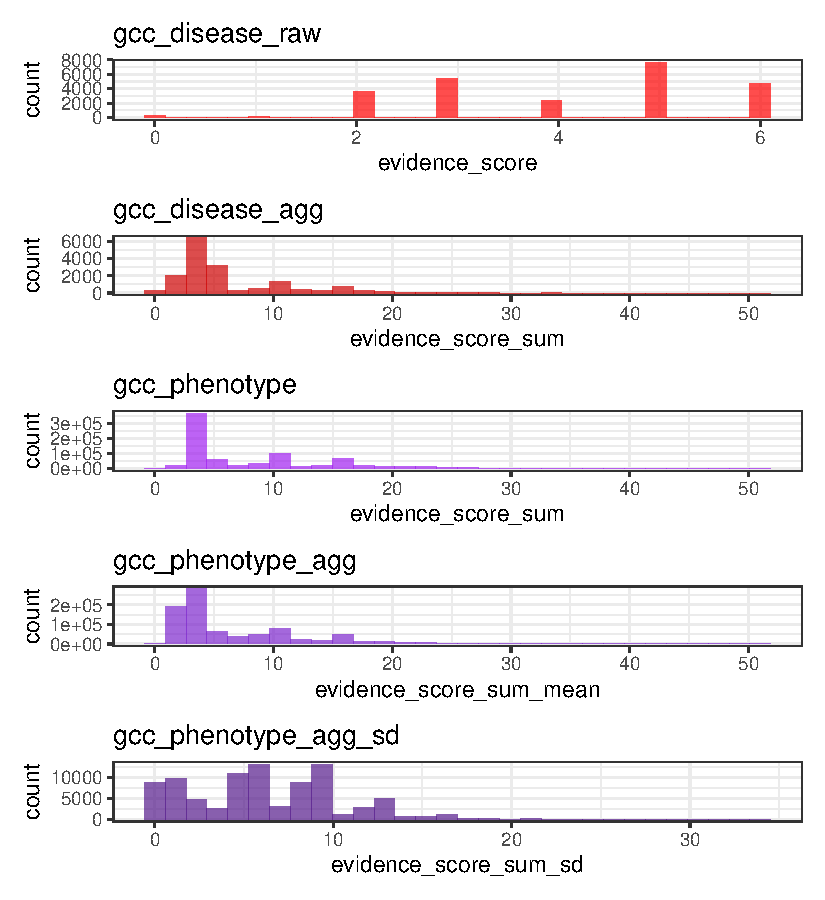
\includegraphics{index_files/figure-pdf/fig-evidence-histograms-1.pdf}

}

\caption{\label{fig-evidence-histogramsD08295A6-16DC-499D-85A8-8BA656E013A2}Distribution
of evidence scores at each processing step.}

\end{figure}%

::: 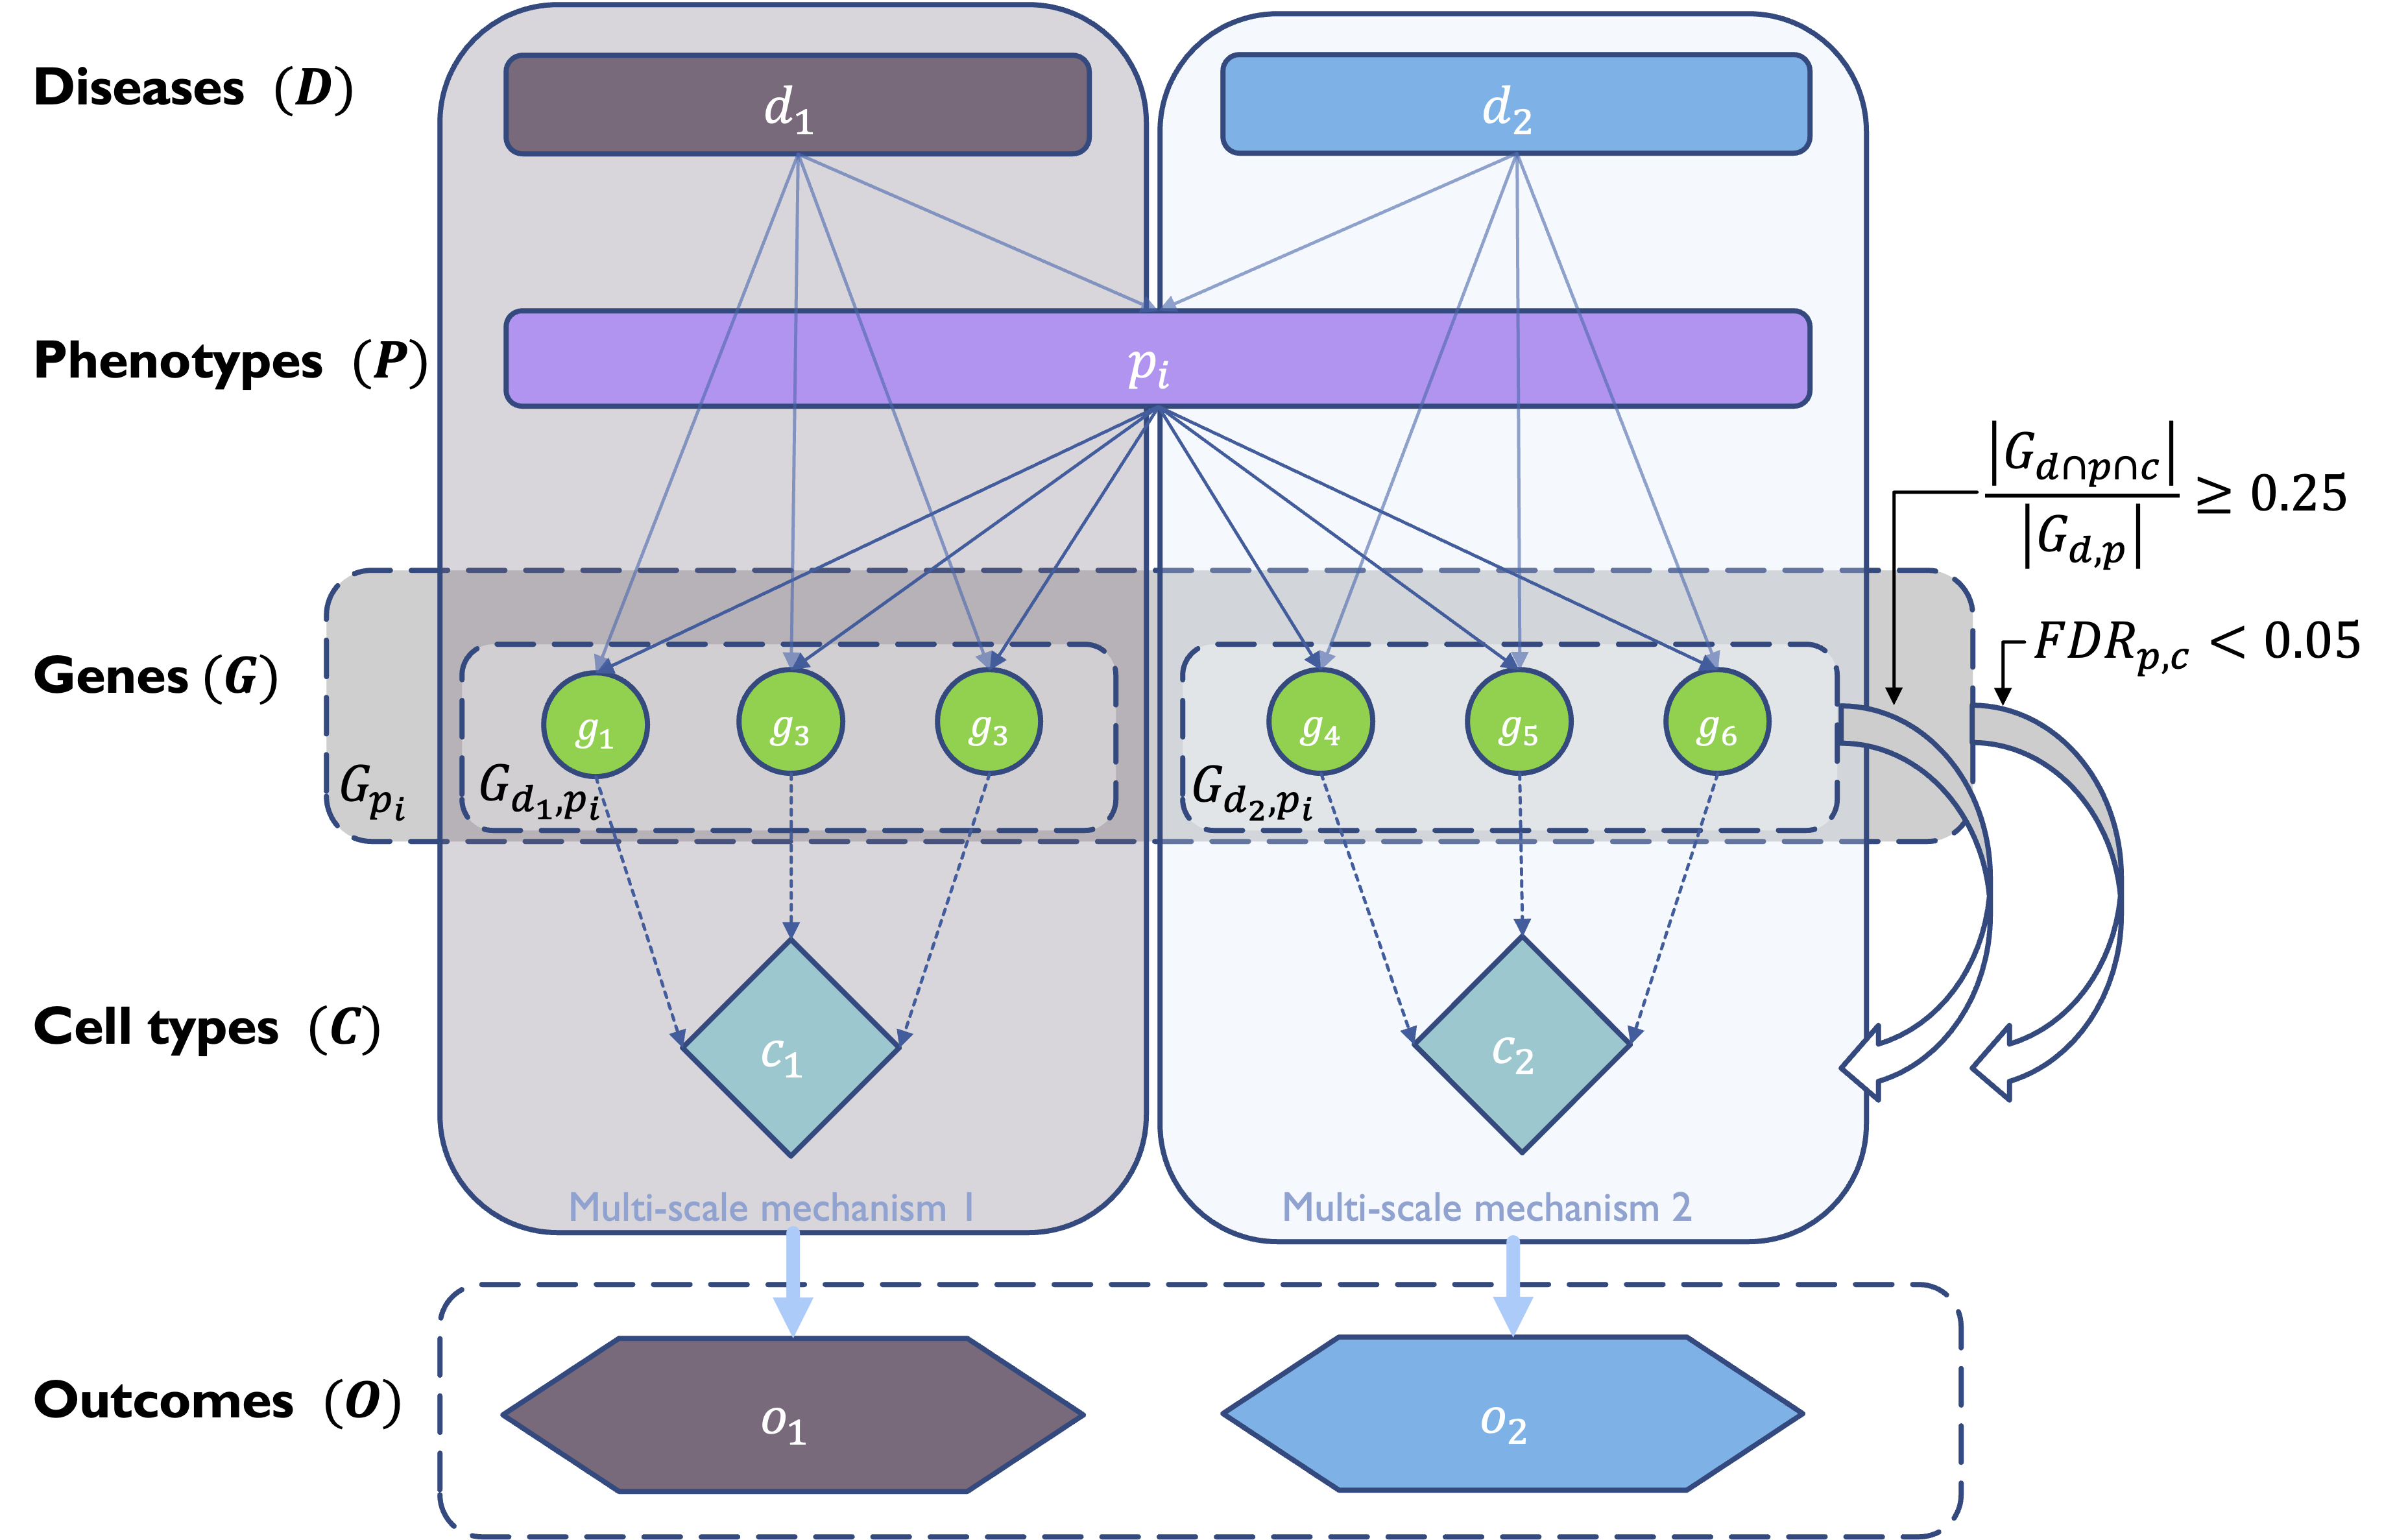
\includegraphics{img/fig-diagram.png}

Diagrammatic overview of multi-scale disease investigation strategy.
Here we provide an abstract example of differential disease aetiology
across multiple scales: diseases (\(D\)), phenotypes (\(P\)), cell types
(\(C\)), genes (\(G\)), and clinical outcomes (\(O\)). In the HPO, genes
are assigned to phenotypes via particular diseases (\(G_{dp}\)).
Therefore, the final gene list for each phenotype is aggregated from
across multiple diseases (\(G_{p}\)). We performed association tests for
all pairwise combinations of cell types and phenotypes and filtered
results after multiple testing corrections (FDR\textless0.05). Each
phenotype in the context of a given disease is referred to here as a
symptom. Links were established between symptoms and cell types through
proportional gene set overlap at a minimum threshold of 25\%. :::

\newpage{}

\begin{figure}[H]

\centering{

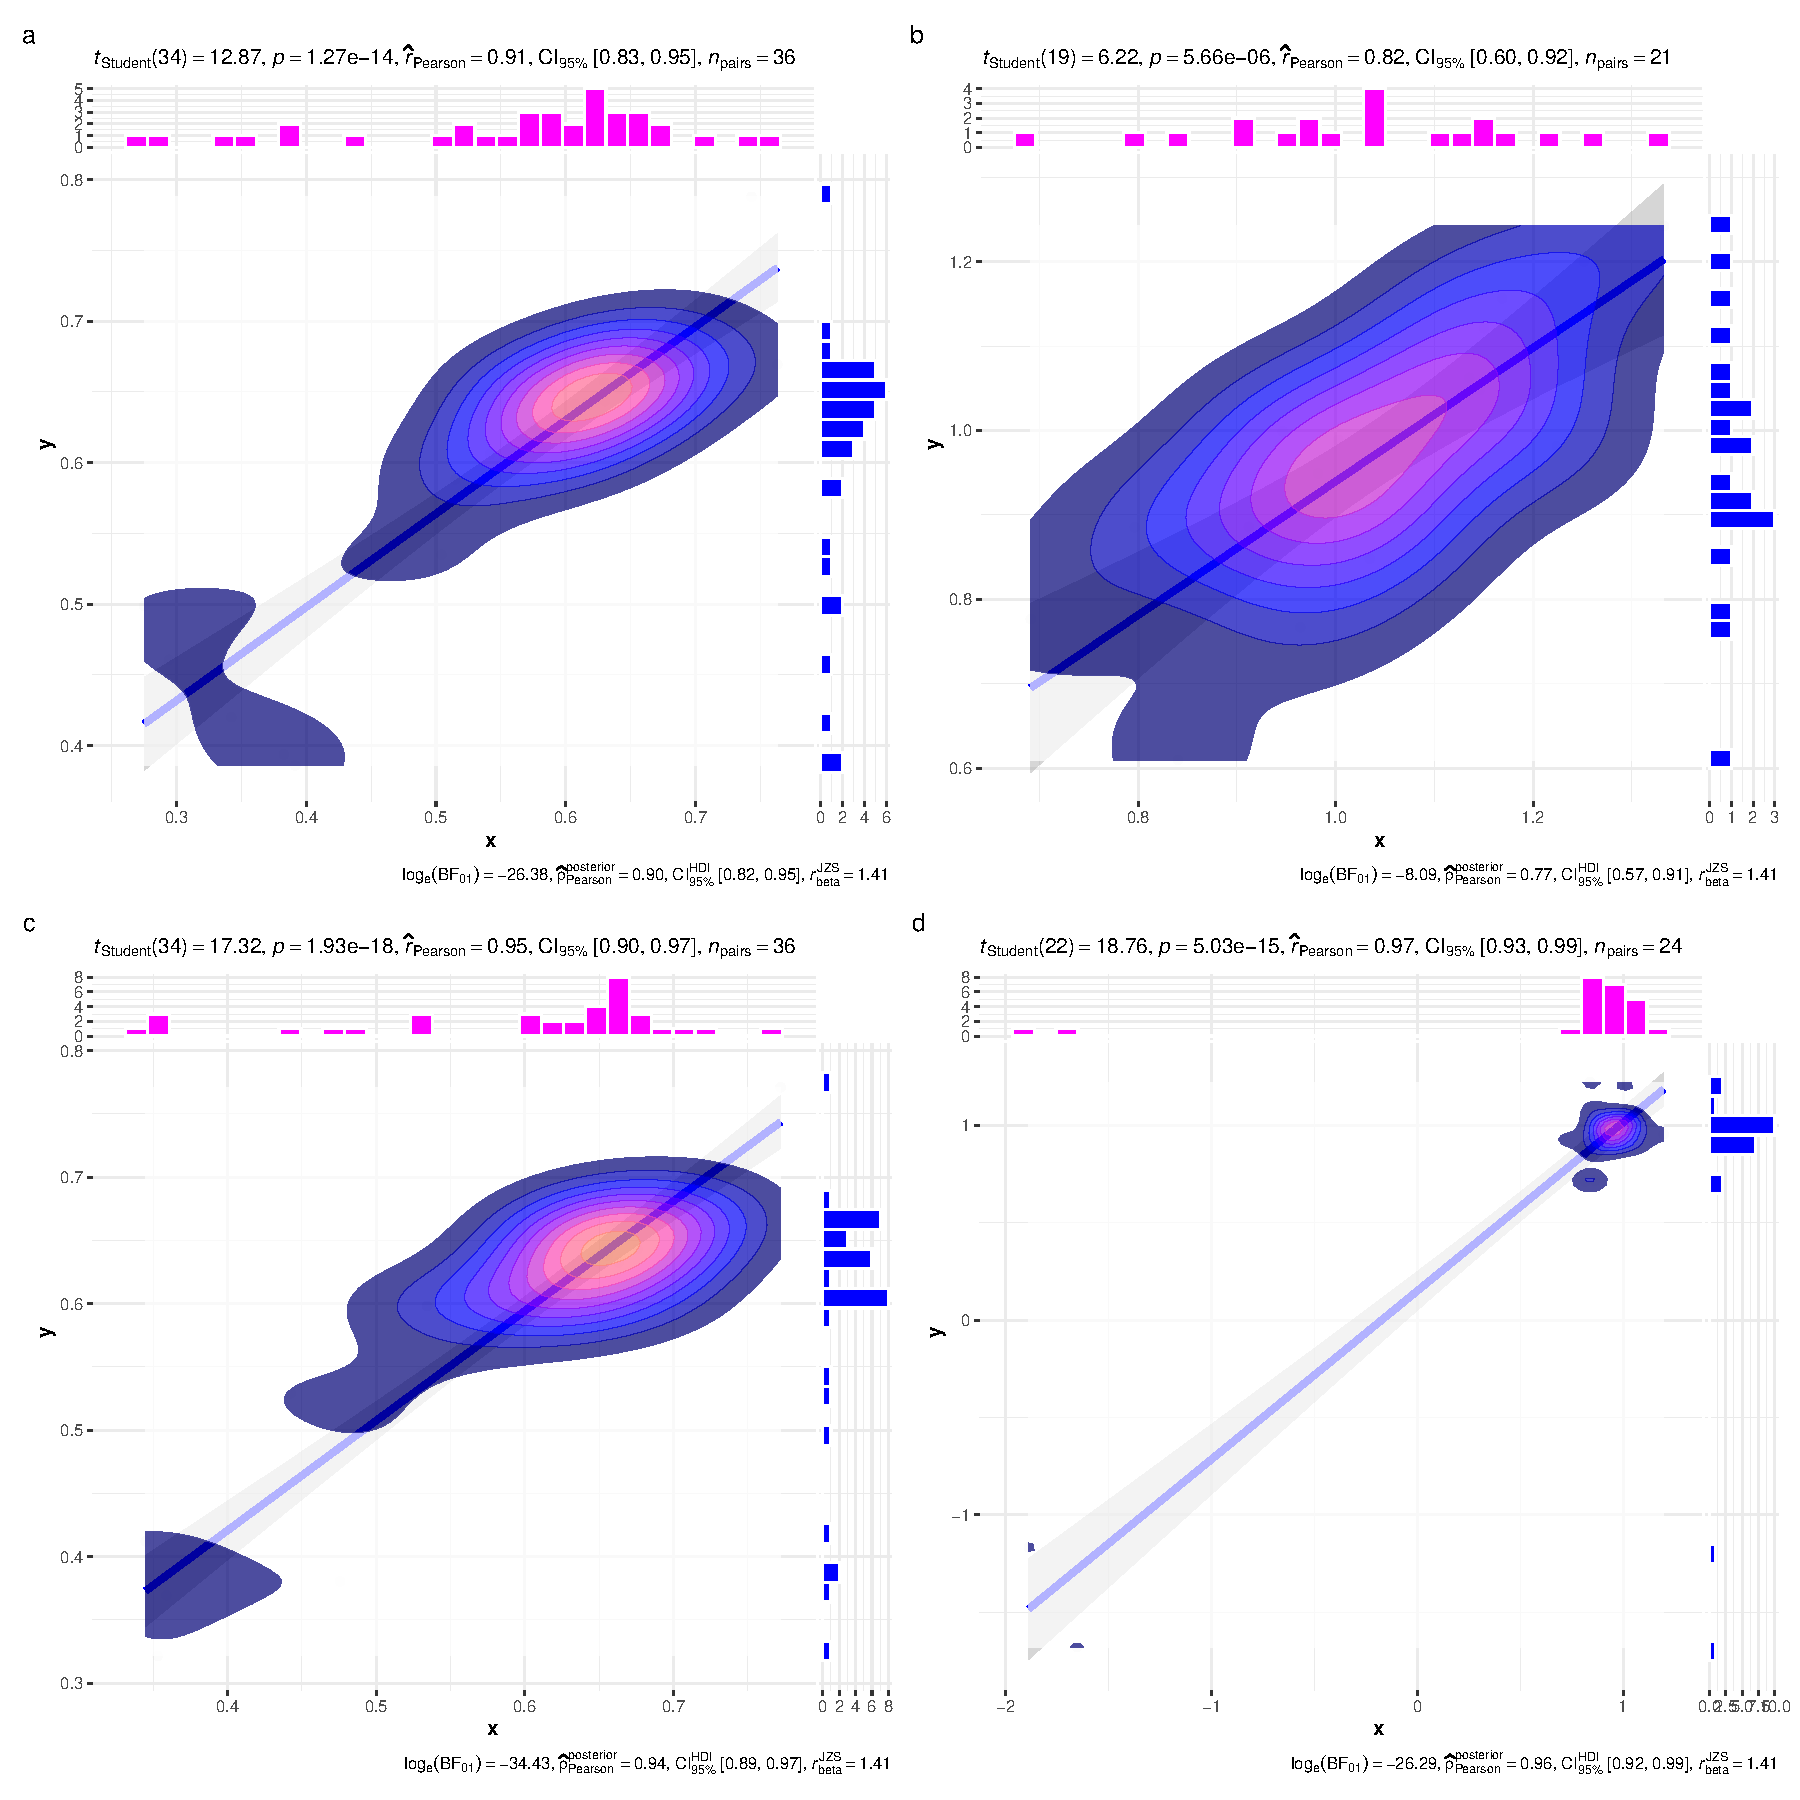
\includegraphics{index_files/figure-pdf/fig-ctd-correlation-1.pdf}

}

\caption{\label{fig-ctd-correlationD08295A6-16DC-499D-85A8-8BA656E013A2}Inter-
and intra-dataset validation across the different CellTypeDataset (CTD)
and developmental stages. Correlations are computed using Pearson
correlation coefficient. Point density is plotted using a 2D kernel
density estimate. \textbf{a} Correlation between the uncorrected
p-values from all phenotype-cell type association tests using the
Descartes Human vs.~Human Cell Landscape CTDs. \textbf{b} Correlation
between the \(log_{10}(fold-change)\) from significant phenotype-cell
type association tests (FDR\textless0.05) using the Descartes Human
vs.~Human Cell Landscape CTDs. \textbf{c} Correlation between the
uncorrected p-values from all phenotype-cell type association tests
using the Human Cell Landscape fetal samples vs.~Human Cell Landscape
adult samples. \textbf{d} Correlation between the
\(log_{10}(fold-change)\) from significant phenotype-cell type
association tests (FDR\textless0.05) using the Human Cell Landscape
fetal samples vs.~Human Cell Landscape adult samples.}

\end{figure}%

\newpage{}

\begin{figure}[H]

\centering{

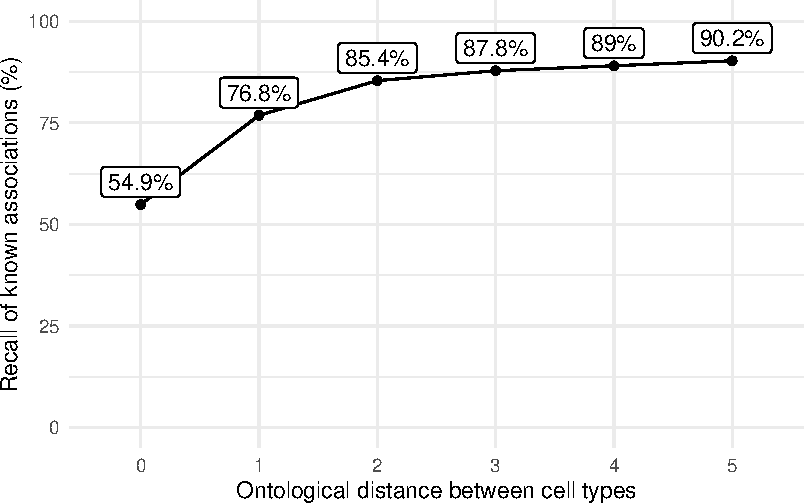
\includegraphics{index_files/figure-pdf/fig-monarch-recall-1.pdf}

}

\caption{\label{fig-monarch-recallD08295A6-16DC-499D-85A8-8BA656E013A2}Recall
of ground-truth Monarch Knowledge Graph phenotype-cell type
relationships at each ontological distance between cell types according
to the Cell Ontology.}

\end{figure}%

\newpage{}

\begin{figure}[H]

\centering{

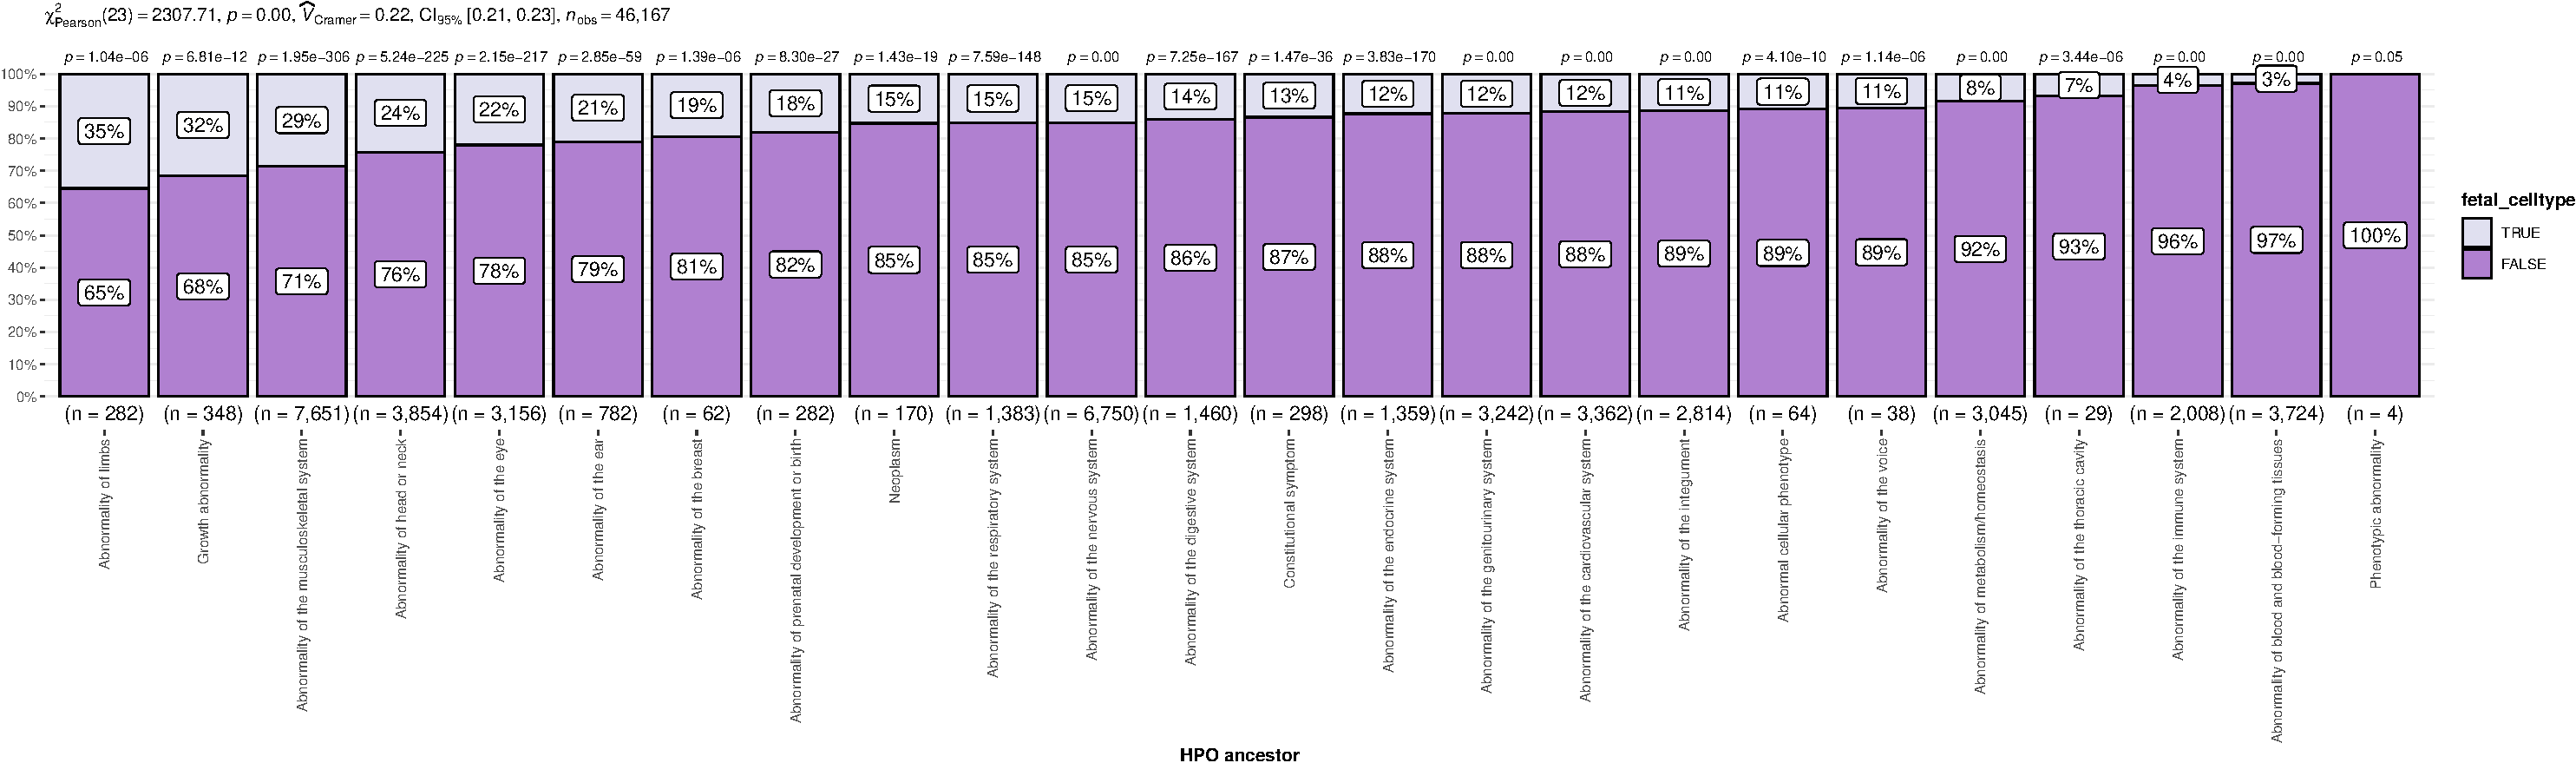
\includegraphics{index_files/figure-pdf/fig-congenital-branches-1.pdf}

}

\caption{\label{fig-congenital-branchesD08295A6-16DC-499D-85A8-8BA656E013A2}The
proportion of cell type-phenotype association tests that are enriched
for foetal cell types within each HPO branch.}

\end{figure}%

\newpage{}

\begin{figure}[H]

\centering{

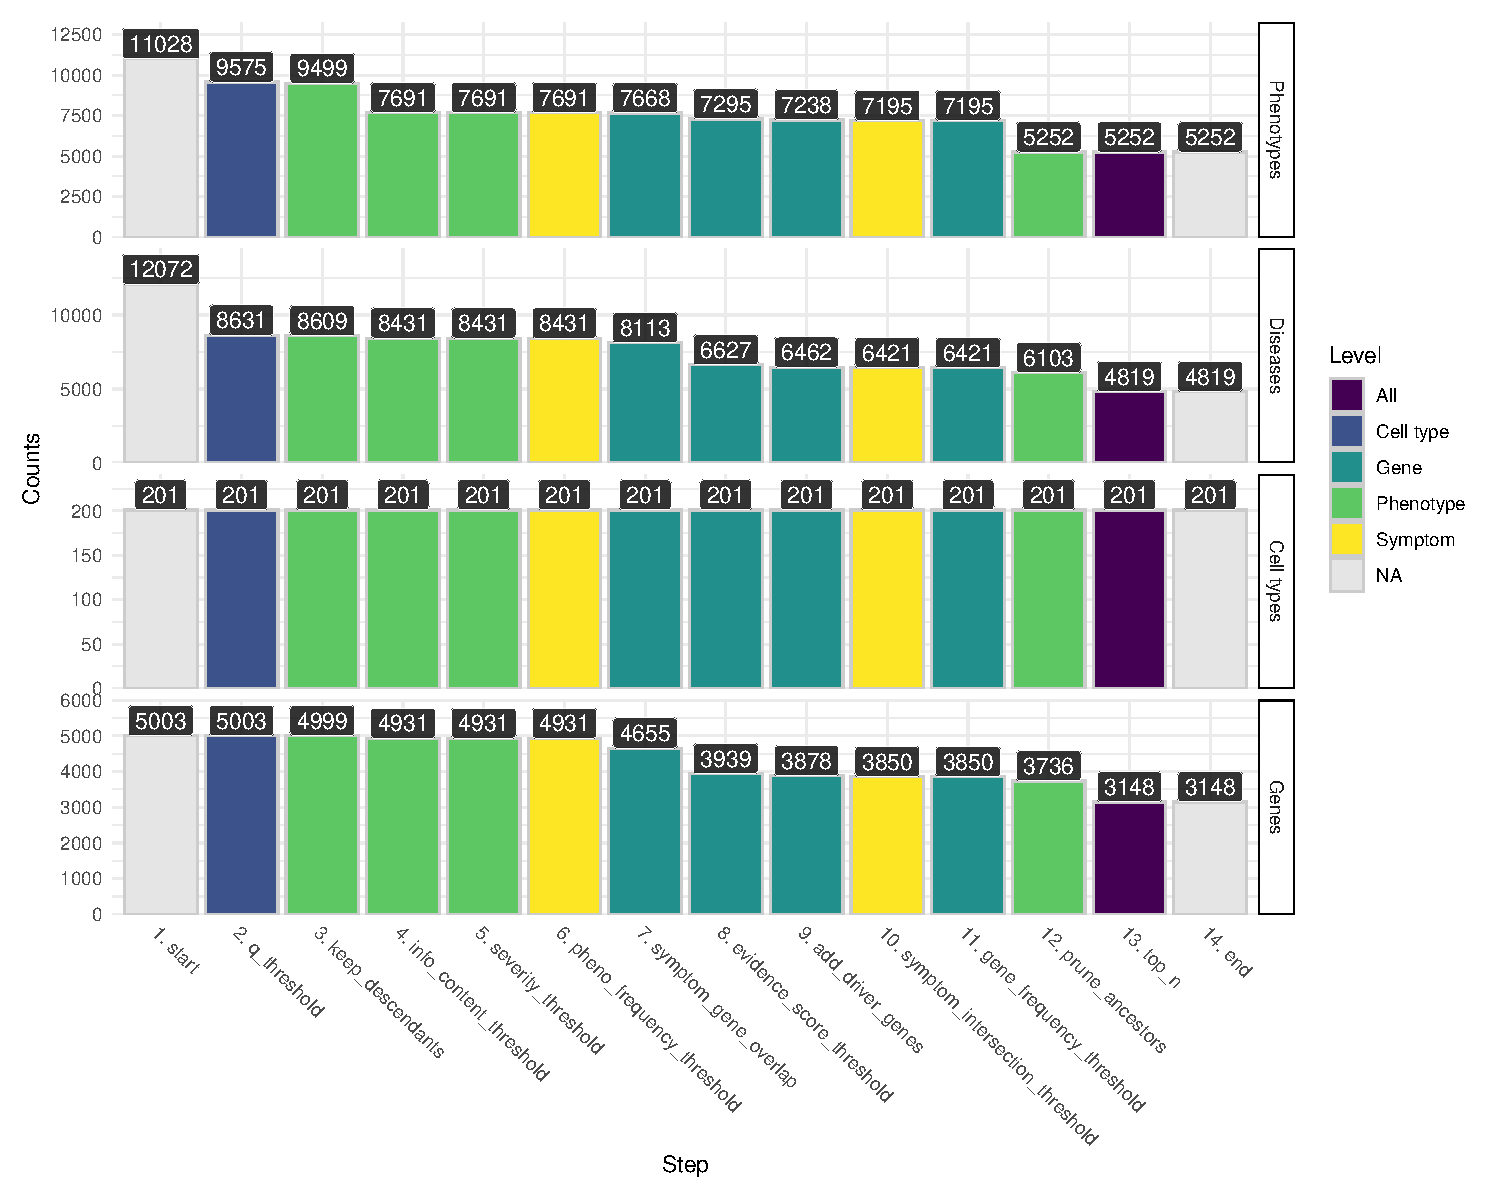
\includegraphics{index_files/figure-pdf/fig-therapy-filter-1.pdf}

}

\caption{\label{fig-therapy-filterD08295A6-16DC-499D-85A8-8BA656E013A2}Prioritised
target filtering steps. This plot visualises the number of unique
phenotype-cell type associations, cell types, genes, and phenotypes
(\emph{y-axis}) at each filtering step (\emph{x-axis}) within the
multi-scale therapeutic target prioritisation pipeline. Each step in the
pipeline can be easily adjusted according to user preference and use
case. See \textbf{?@tbl-filters} for descriptions and criterion of each
filtering step.}

\end{figure}%

\newpage{}

\begin{figure}[H]

\centering{

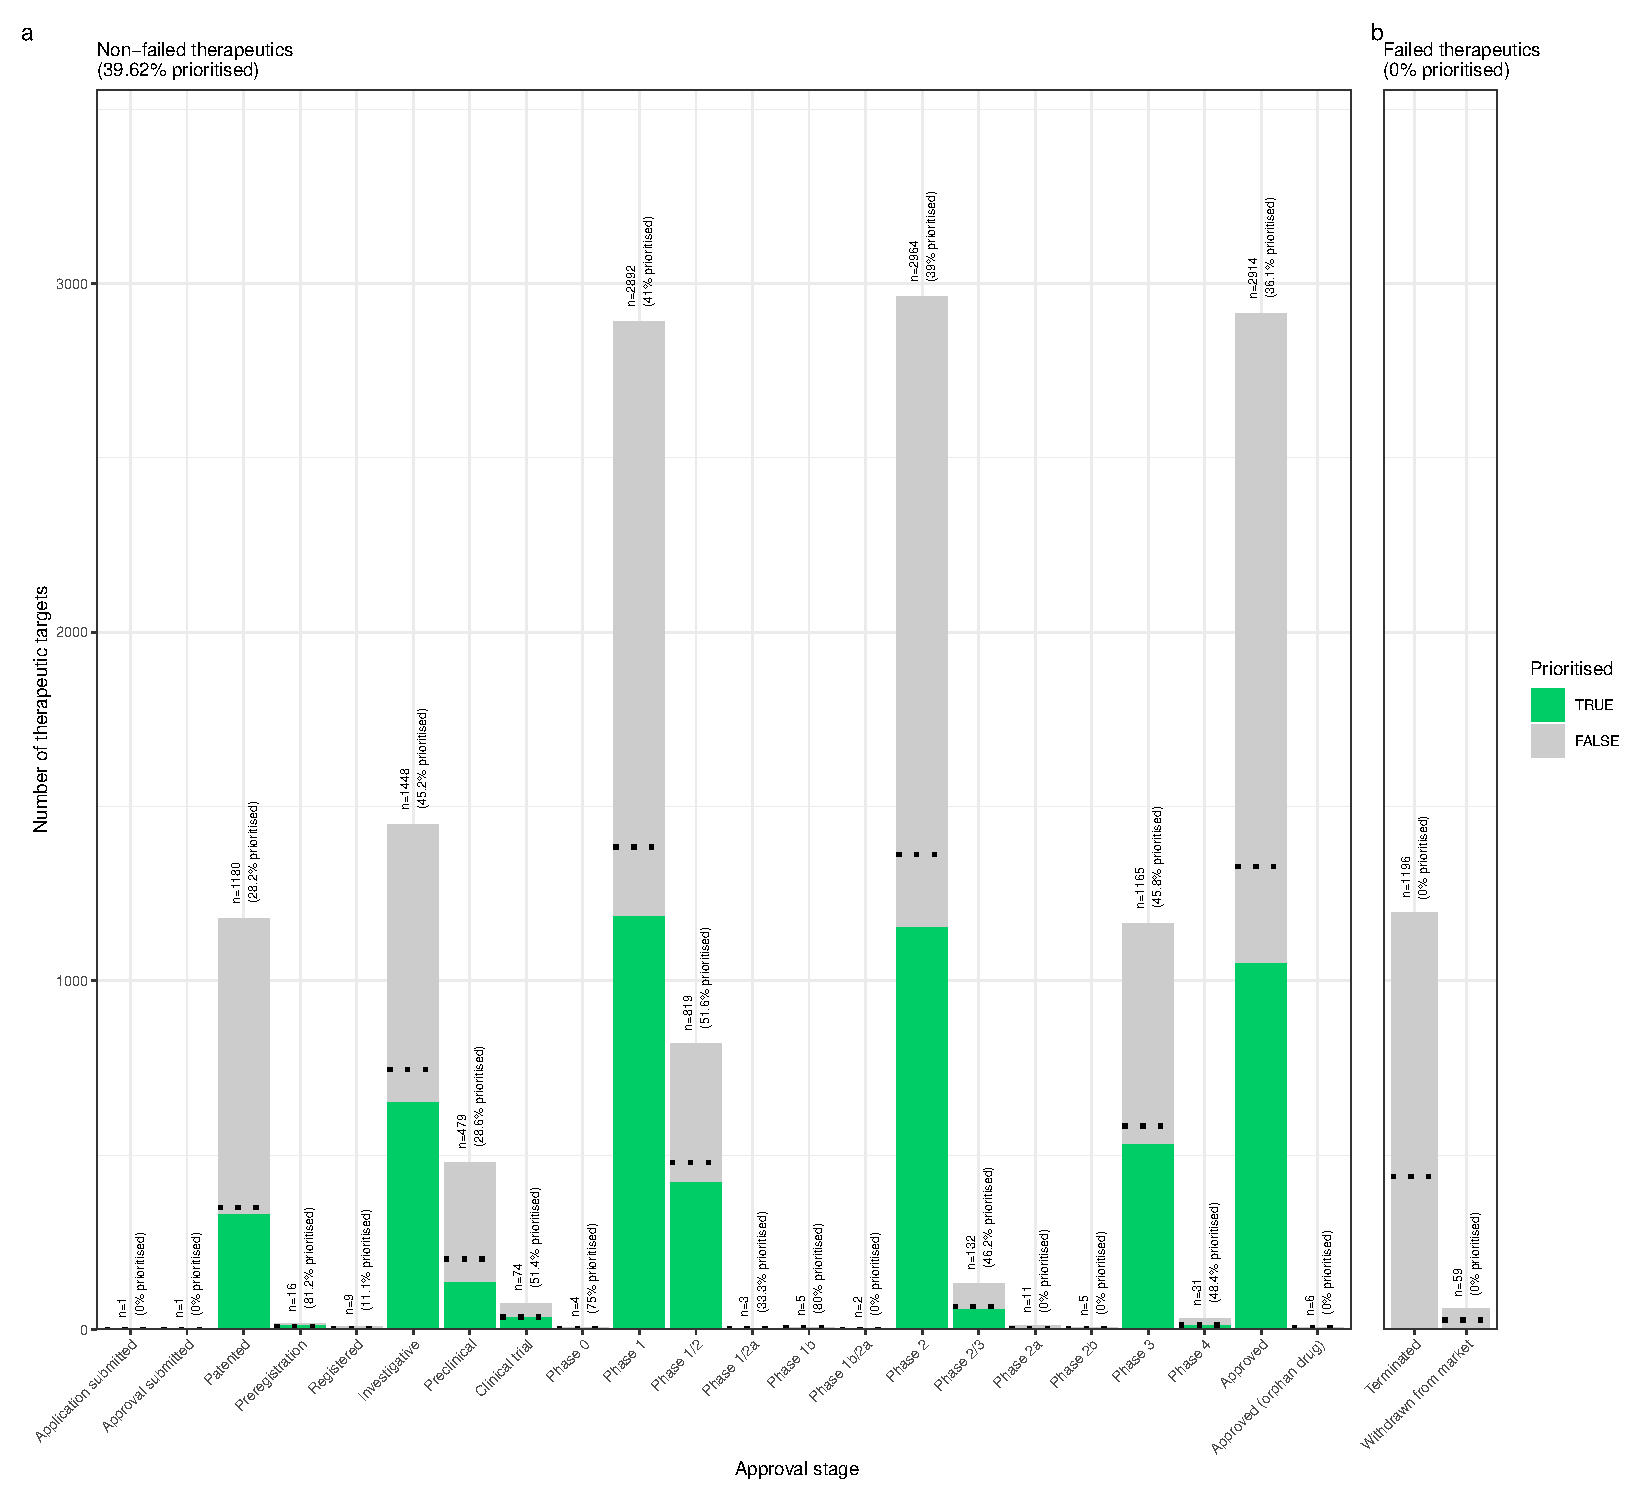
\includegraphics{index_files/figure-pdf/fig-therapy-validate-all-1.pdf}

}

\caption{\label{fig-therapy-validate-allD08295A6-16DC-499D-85A8-8BA656E013A2}Therapeutics
- Validation of prioritised therapeutic targets. Proportion of existing
all therapy targets (documented in the Therapeutic Target Database)
recapitulated by our prioritisation pipeline.}

\end{figure}%

\newpage{}

\begin{figure}[H]

\centering{

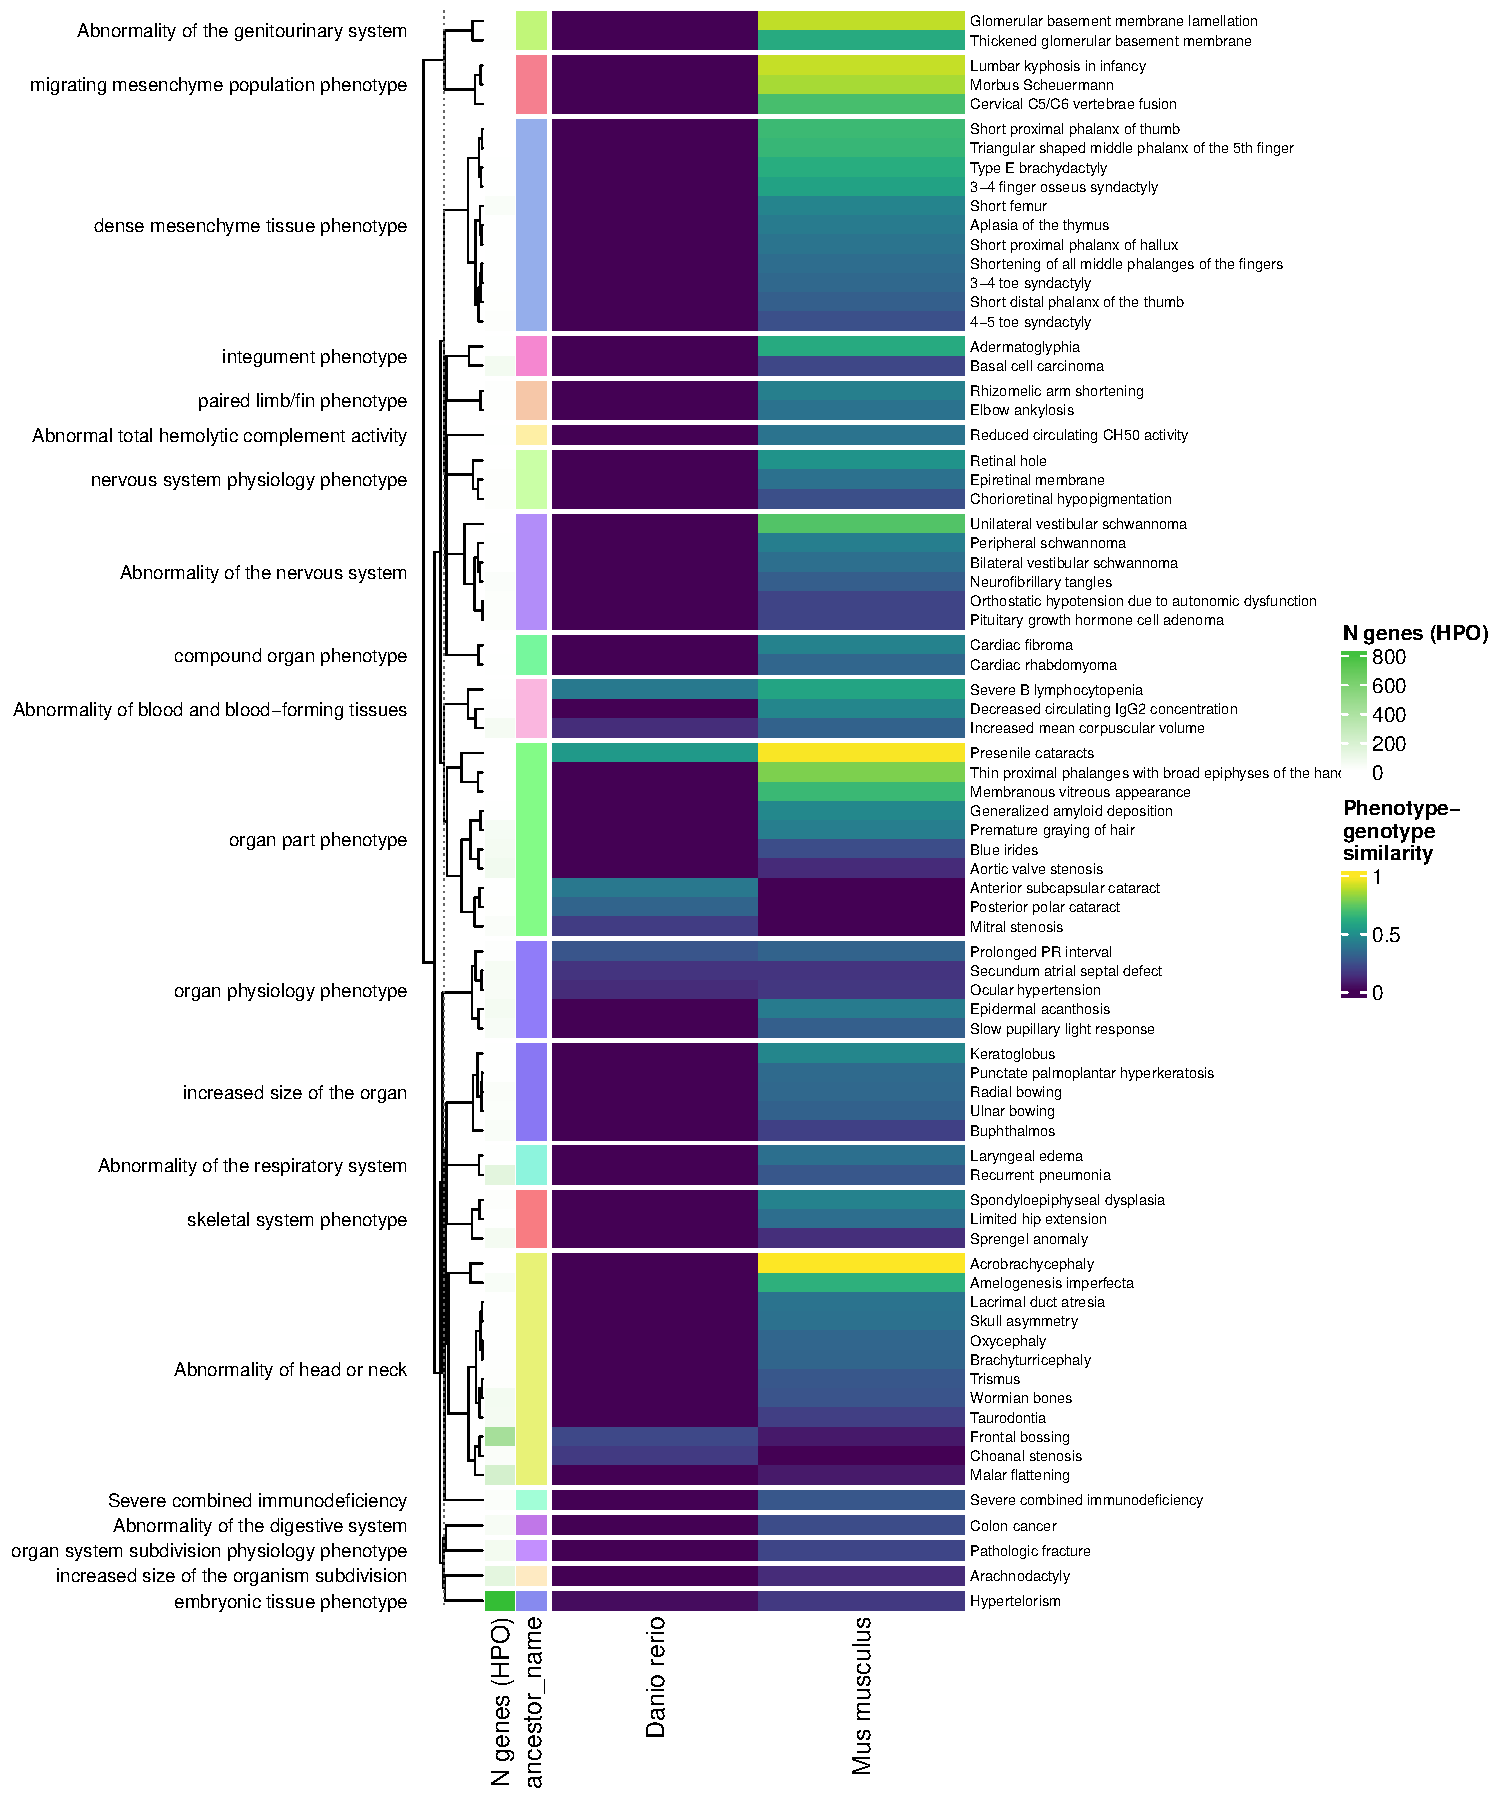
\includegraphics{index_files/figure-pdf/fig-animal-models-1.pdf}

}

\caption{\label{fig-animal-modelsD08295A6-16DC-499D-85A8-8BA656E013A2}Identification
of translatable experimental models. Interspecies translatability of
human phenotypes nominated by the gene therapy prioritised pipeline.
Above, the combined ontological-genotypic similarity score
(\(SIM_{o,g}\)) is displayed as the heatmap fill colour stratified by
the model organism (\emph{x-axis}). An additional column
(``n\_genes\_db1'' on the far left) displays the total number of unique
genes annotated to the phenotypic within the HPO. Phenotypes are
clustered according to their ontological similarity in the HPO
(\emph{y-axis}).}

\end{figure}%

\newpage{}

\begin{figure}

\centering{

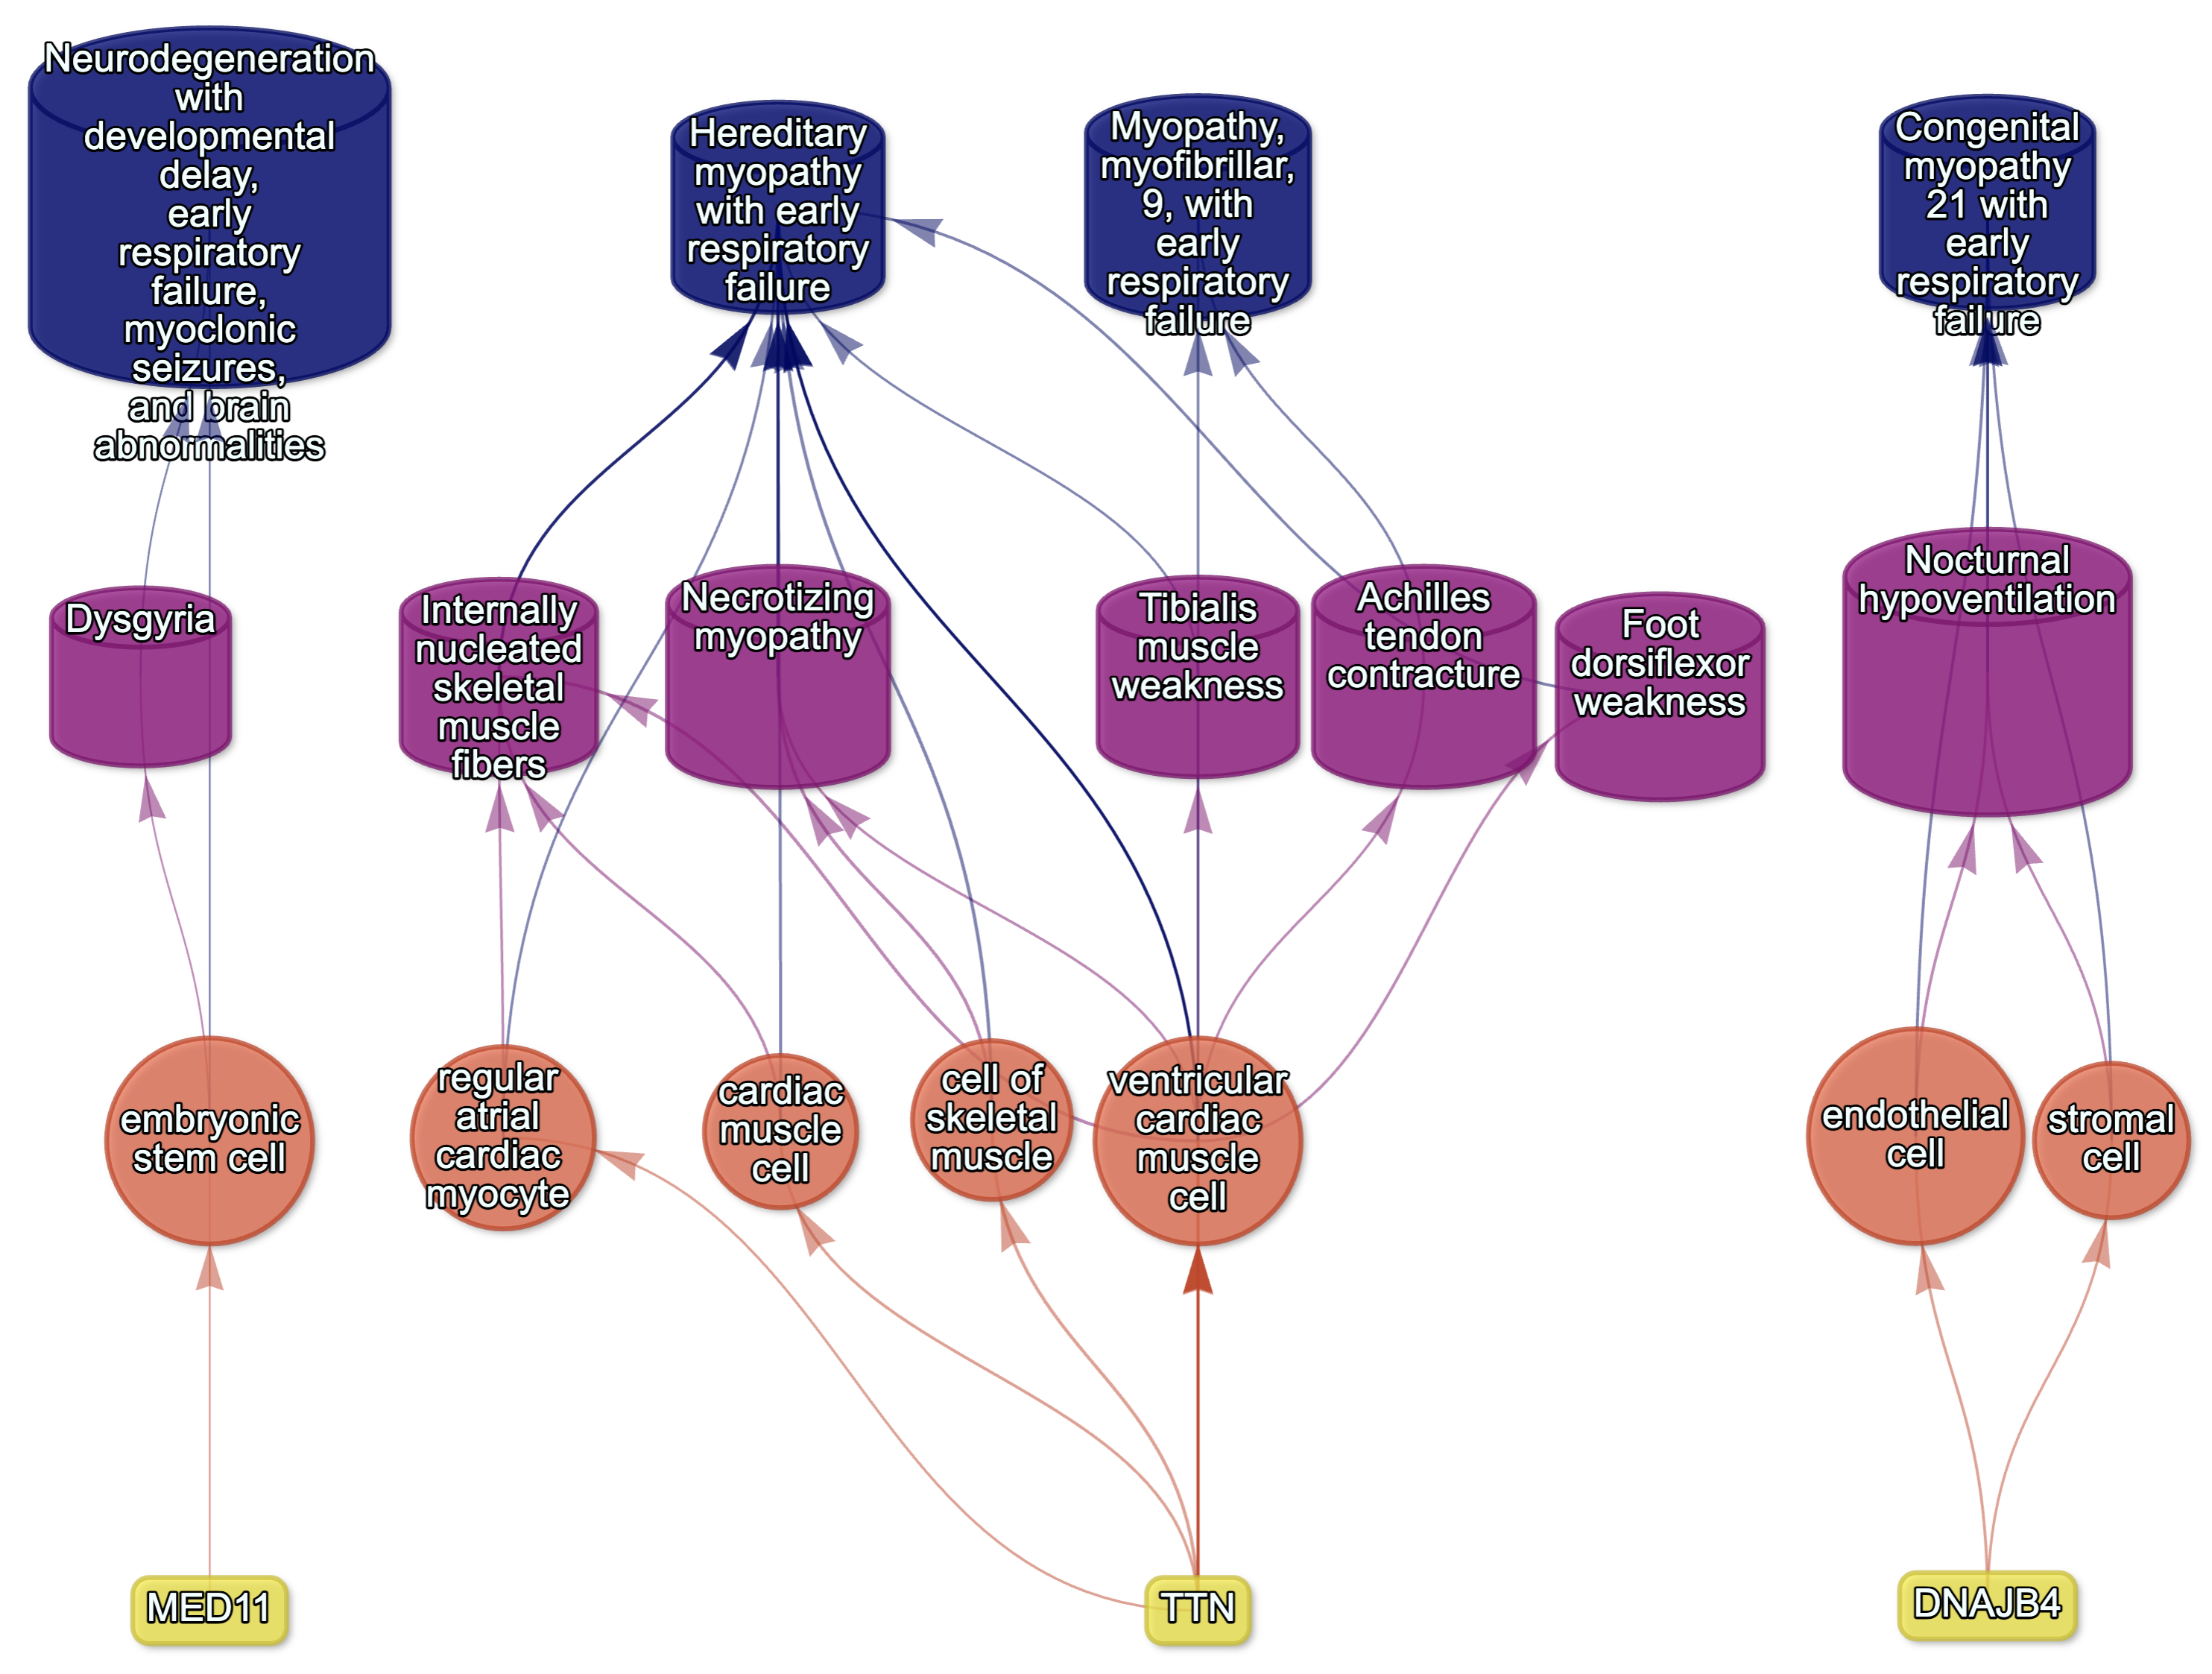
\includegraphics{img/fig-therapy-examples-supp/respiratory_failure.png}

}

\caption{\label{fig-therapy-examples-supp}Respiratory failure}

\end{figure}%

\newpage{}

\begin{figure}

\centering{

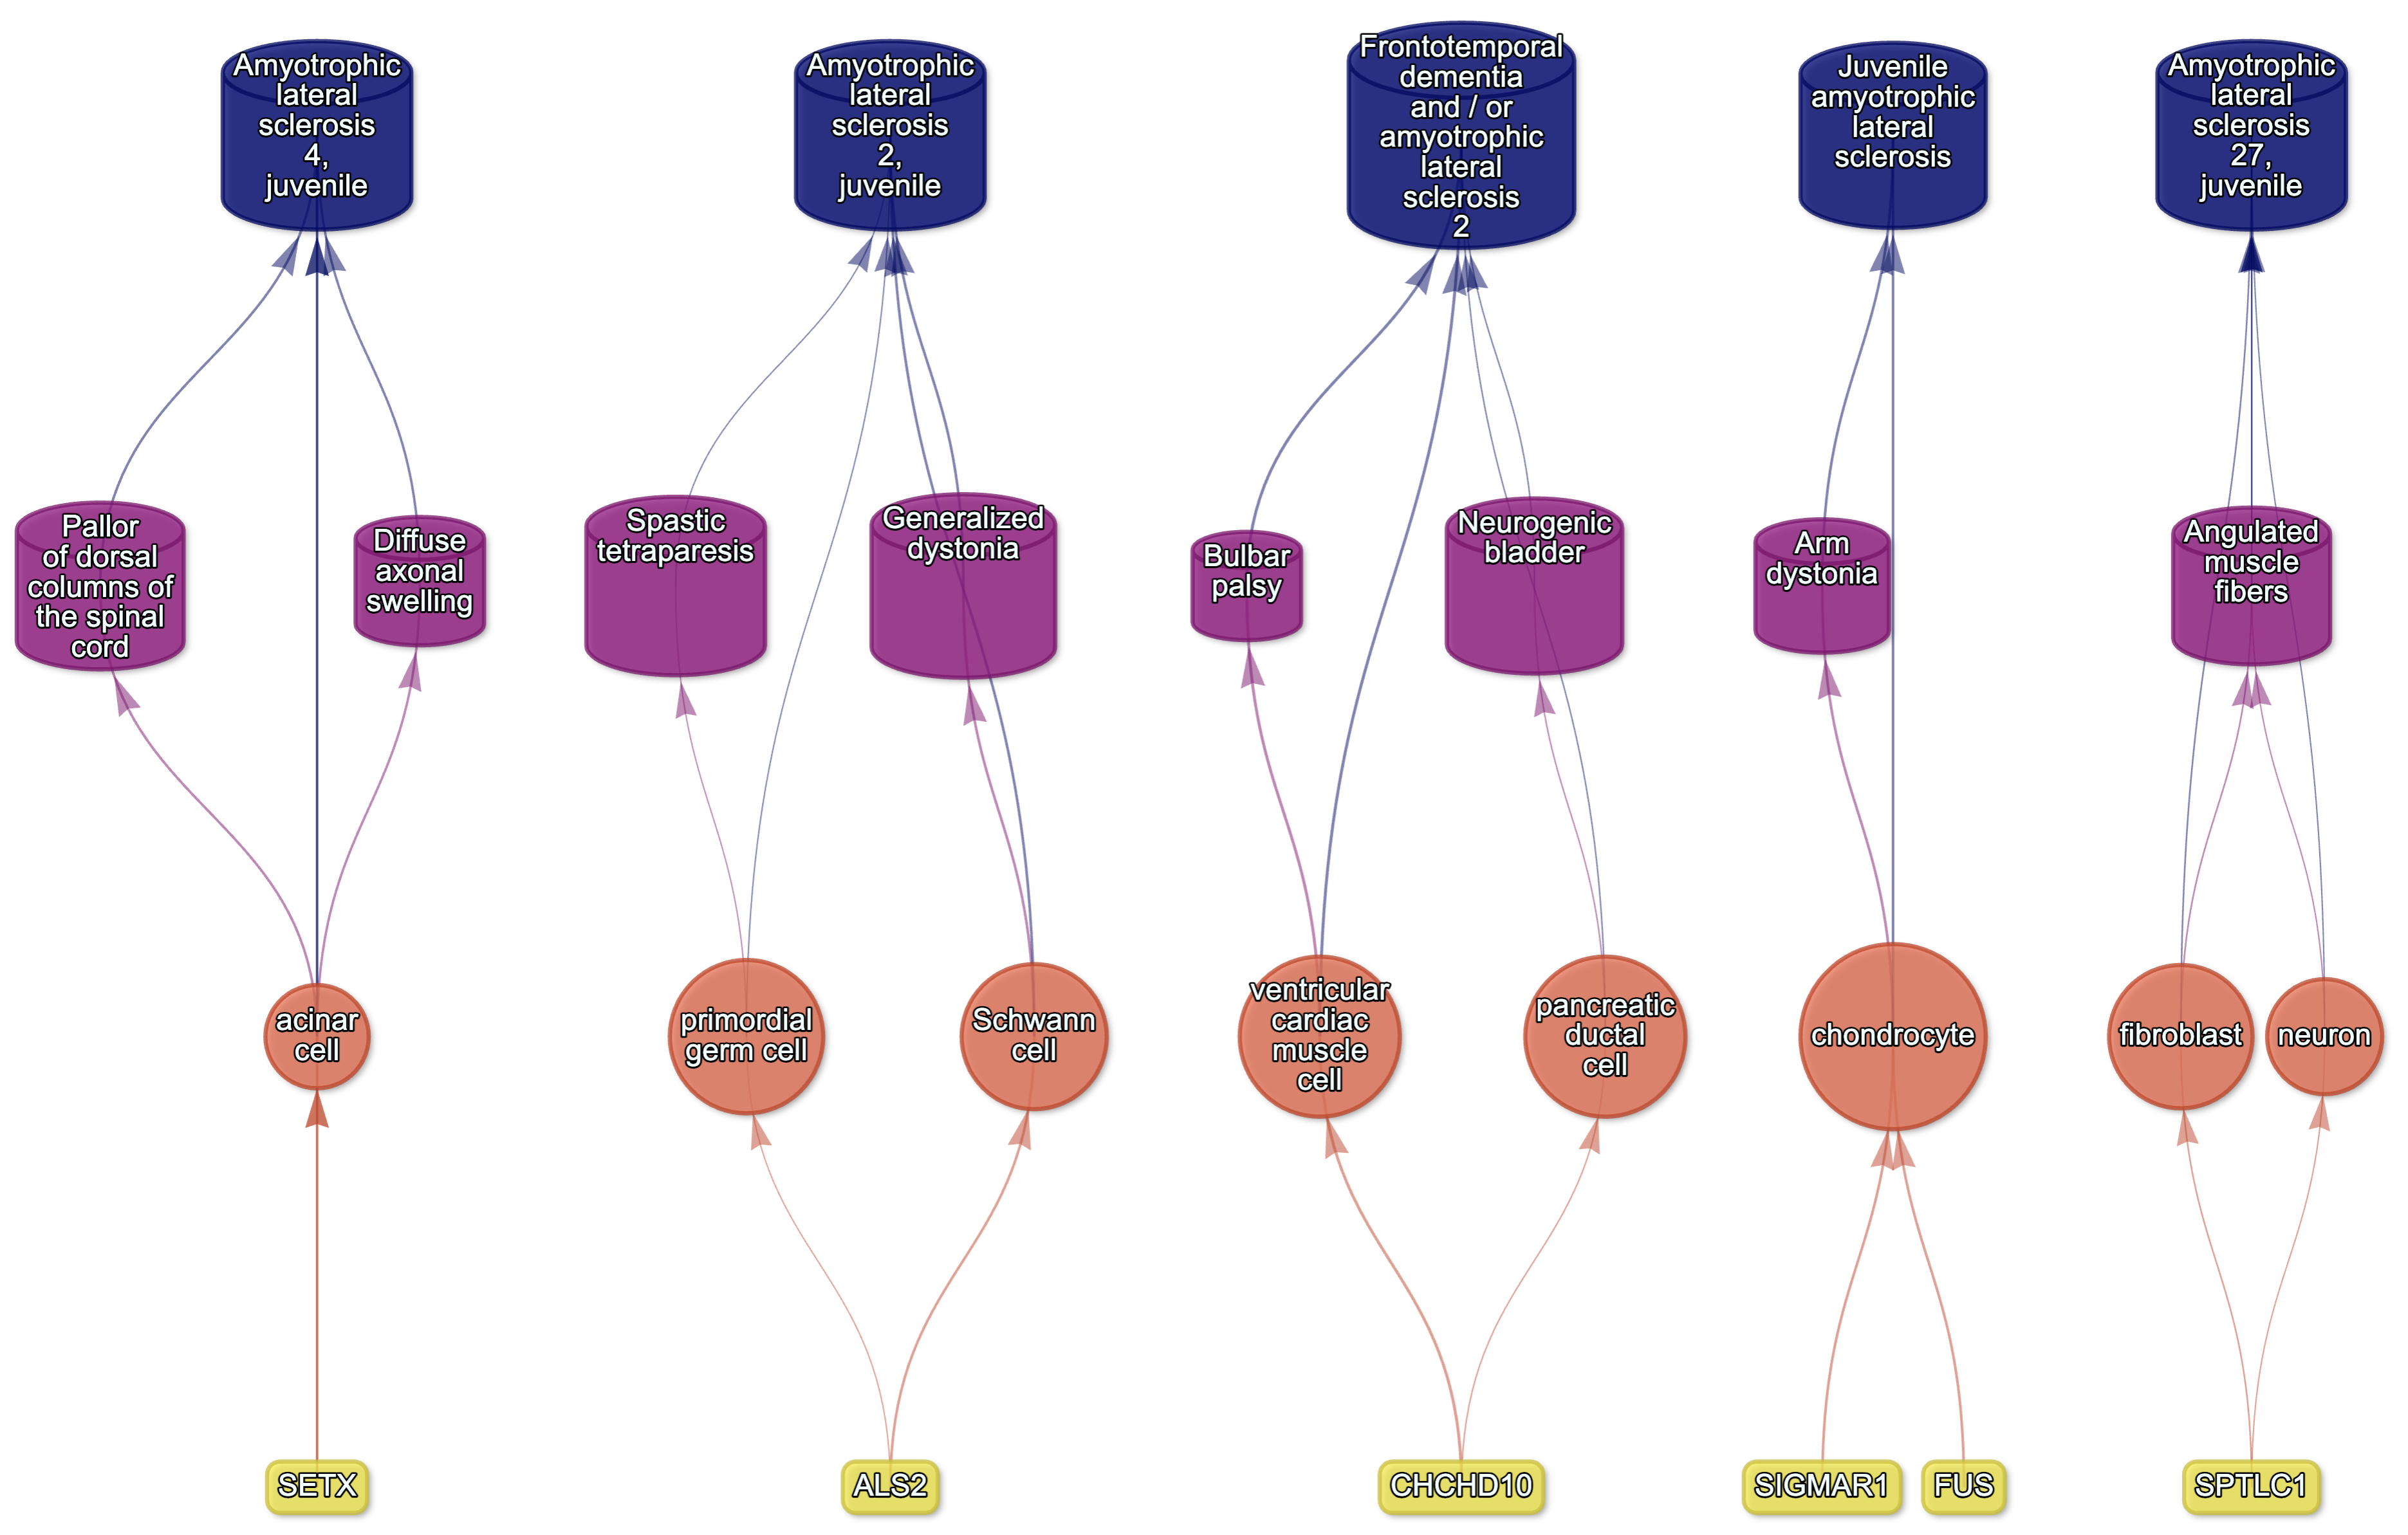
\includegraphics{img/fig-therapy-examples-supp/als.png}

}

\caption{\label{fig-therapy-examples-supp-b}Amyotrophic lateral
sclerosis}

\end{figure}%

\newpage{}

\begin{figure}

\centering{

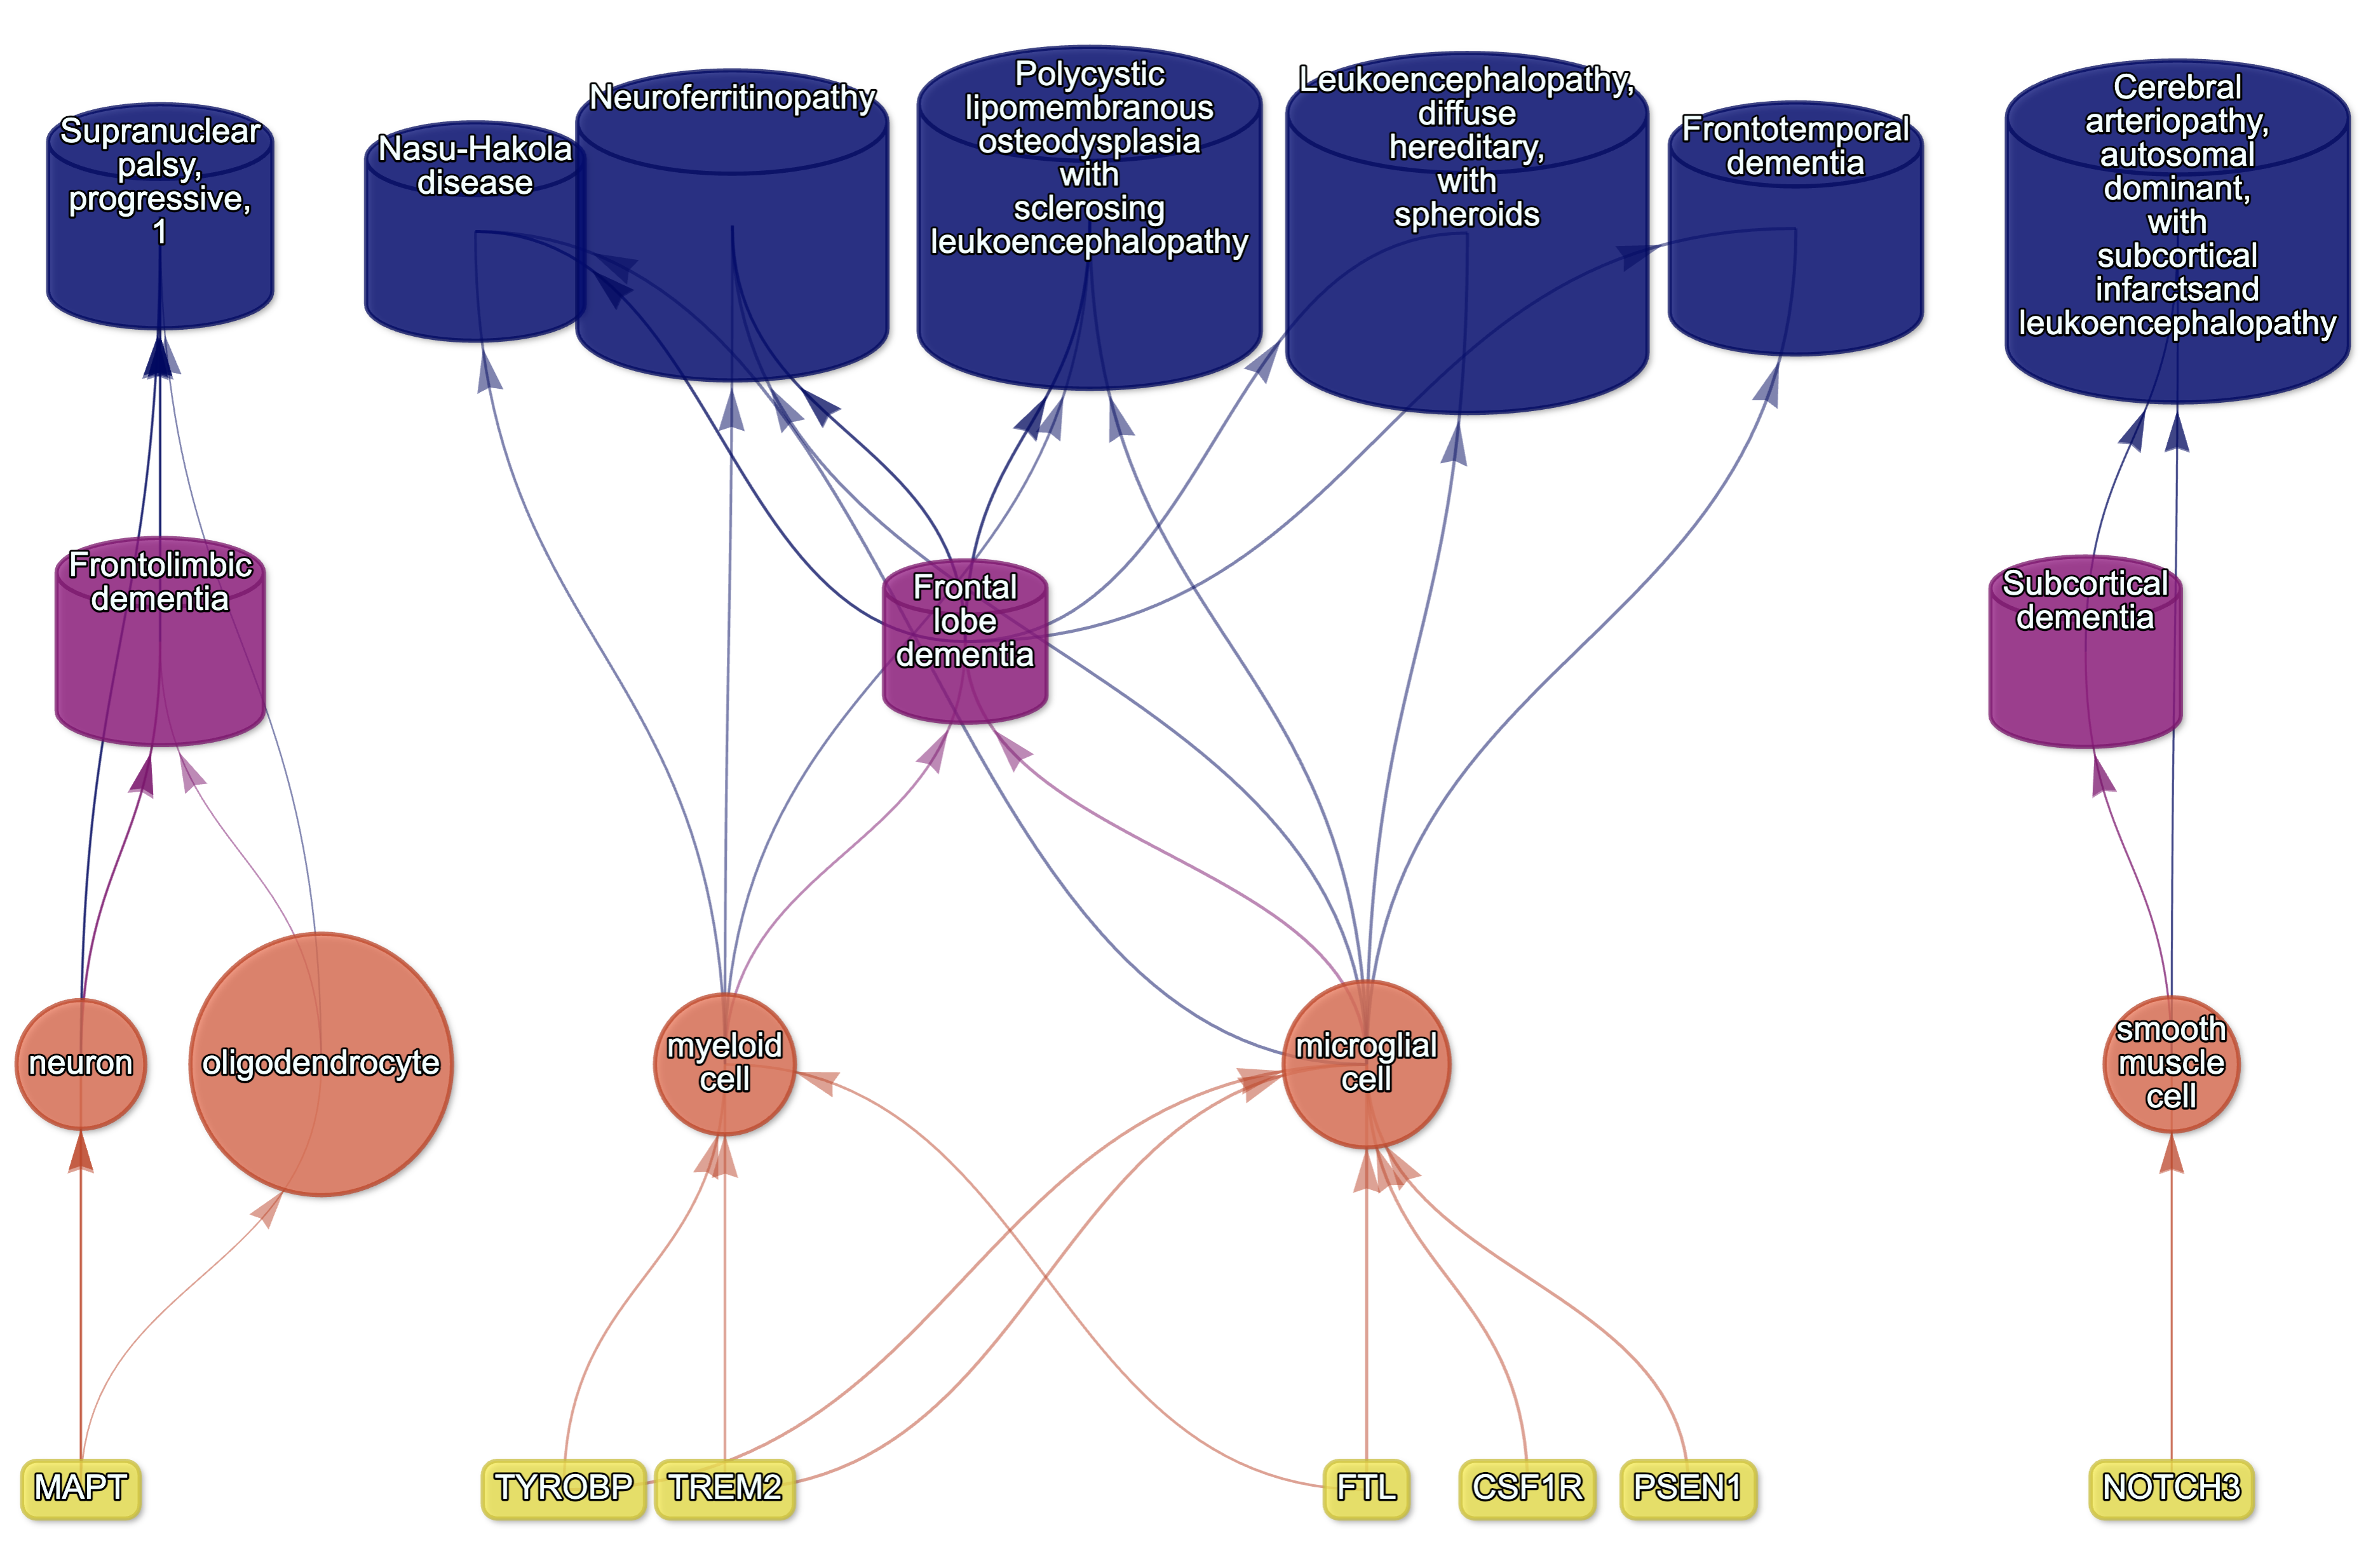
\includegraphics{img/fig-therapy-examples-supp/dementia.png}

}

\caption{\label{fig-therapy-examples-supp-c}Dementia}

\end{figure}%

\newpage{}

\begin{figure}

\centering{

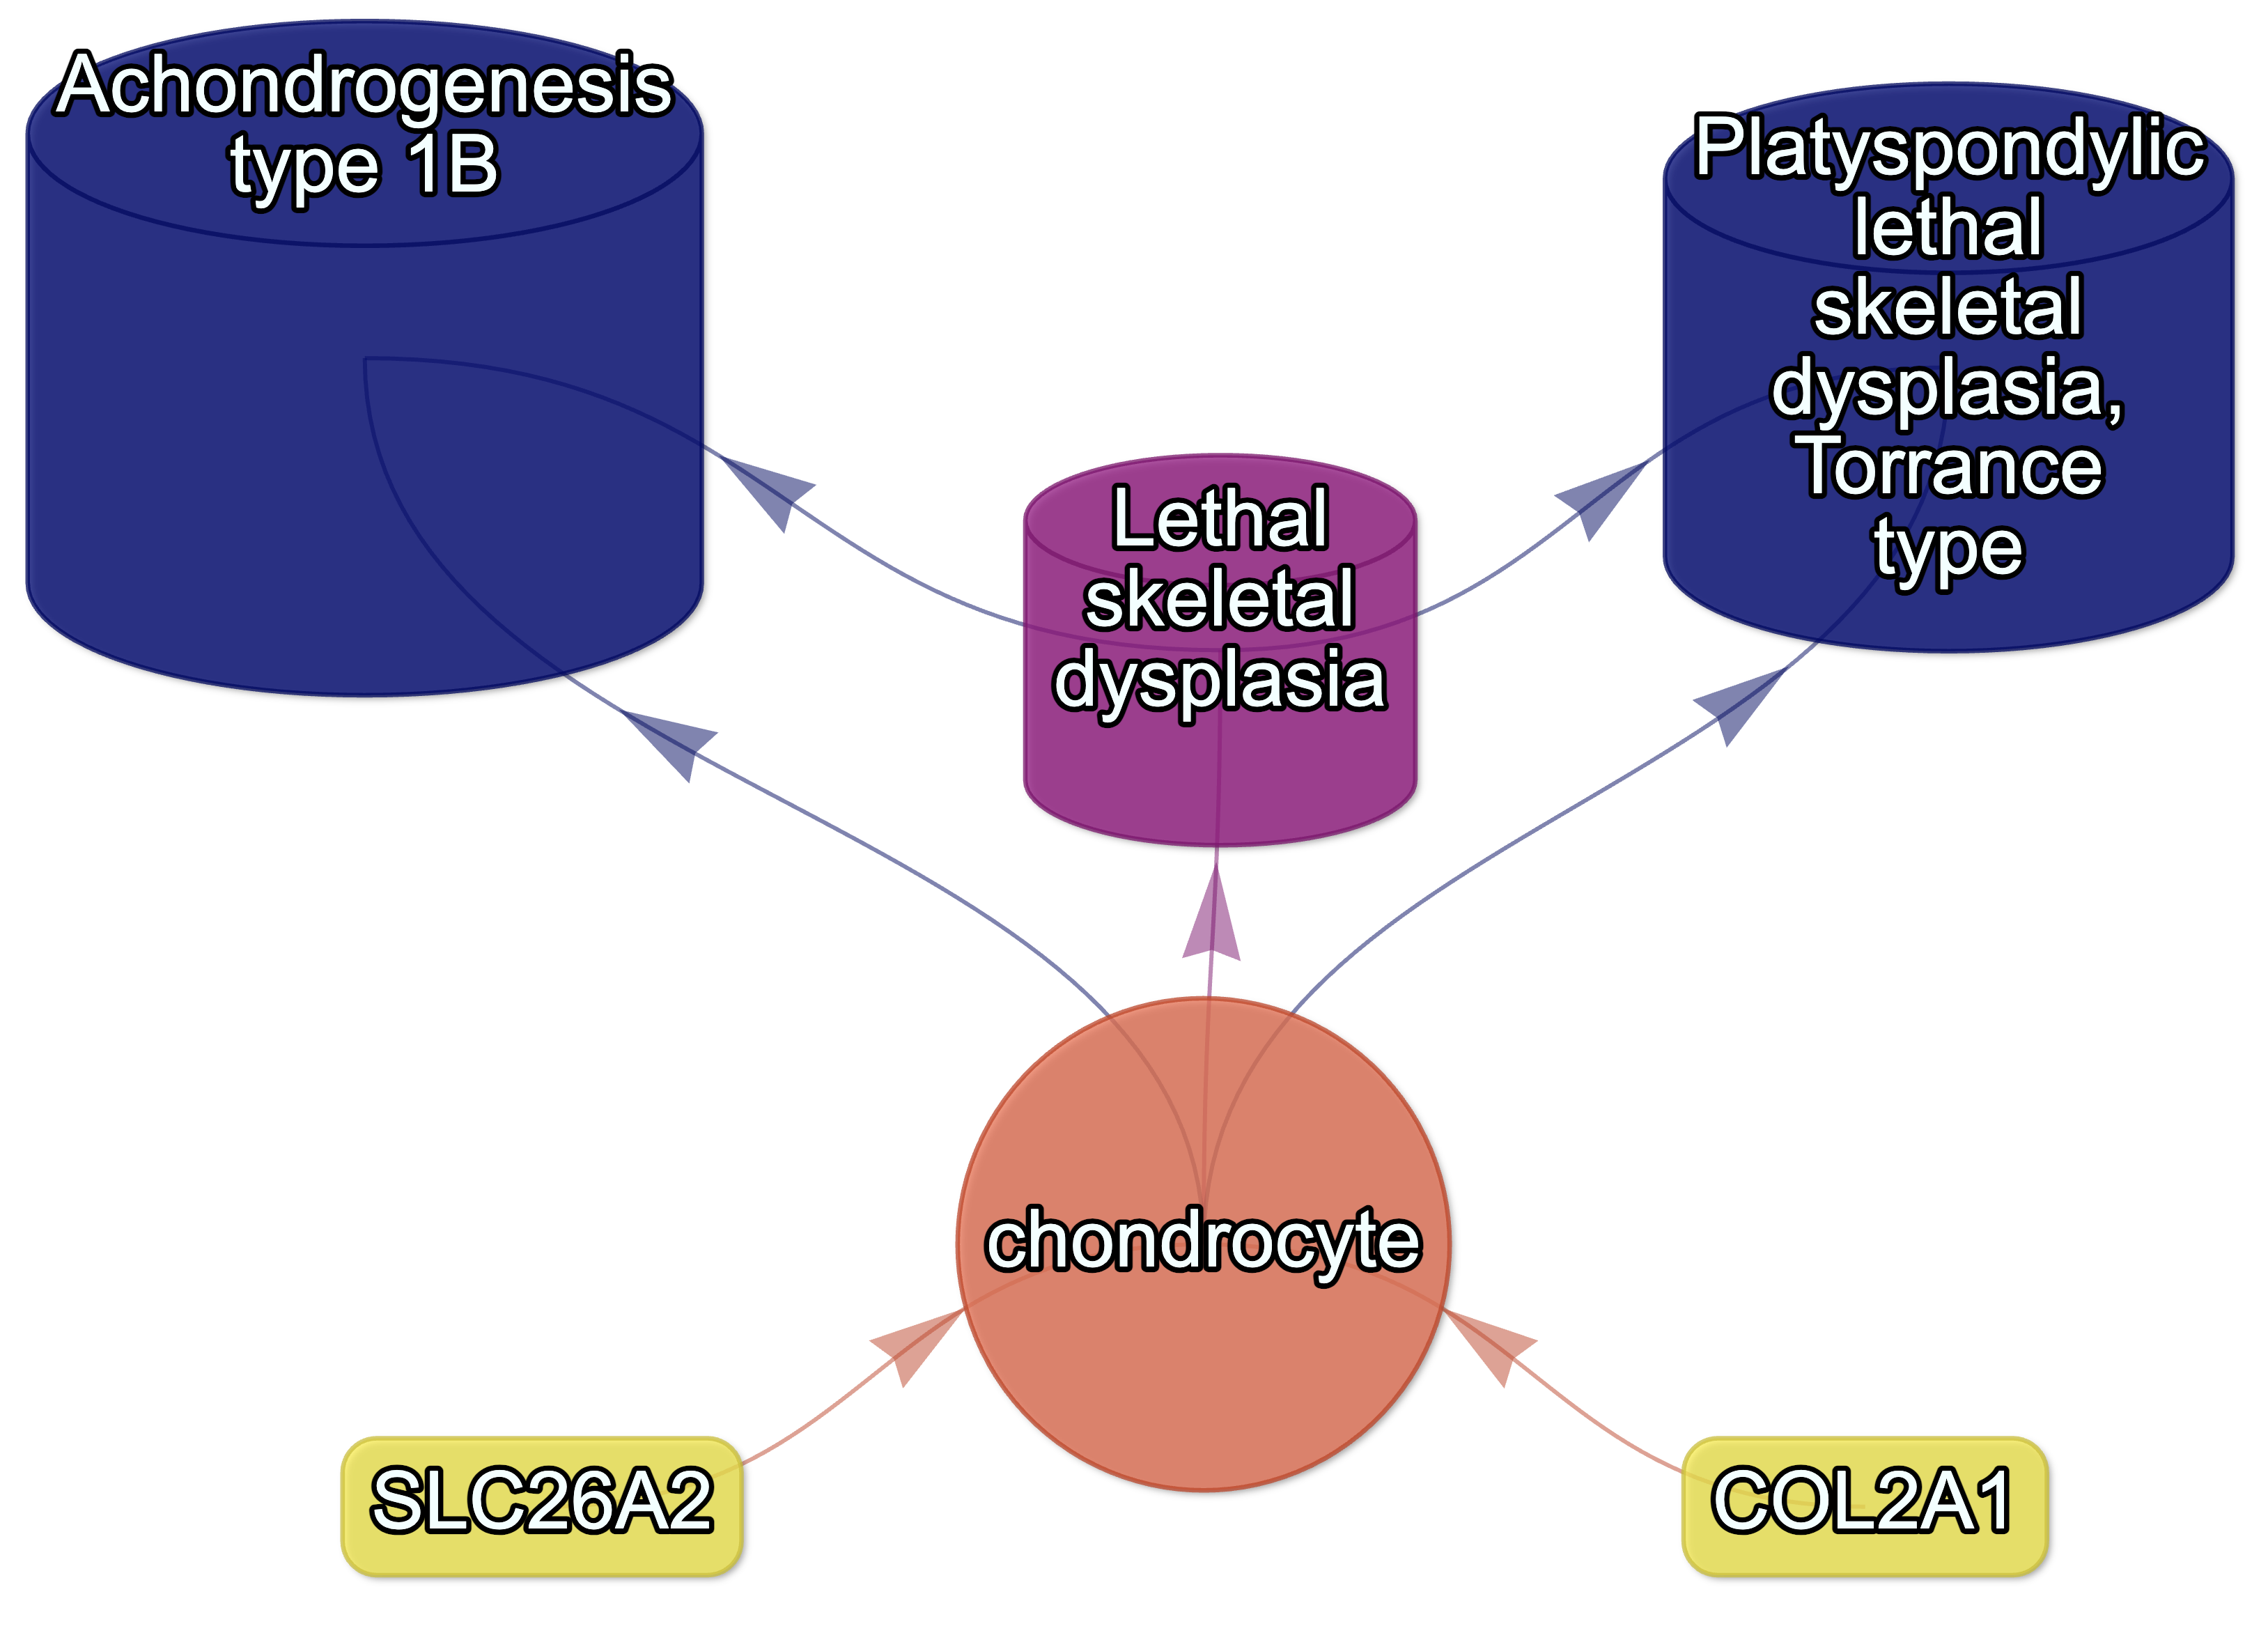
\includegraphics{img/fig-therapy-examples-supp/lethal_skeletal_dysplasia.png}

}

\caption{\label{fig-therapy-examples-supp-d}Lethal skeletal dysplasia}

\end{figure}%

\newpage{}

\begin{figure}

\centering{

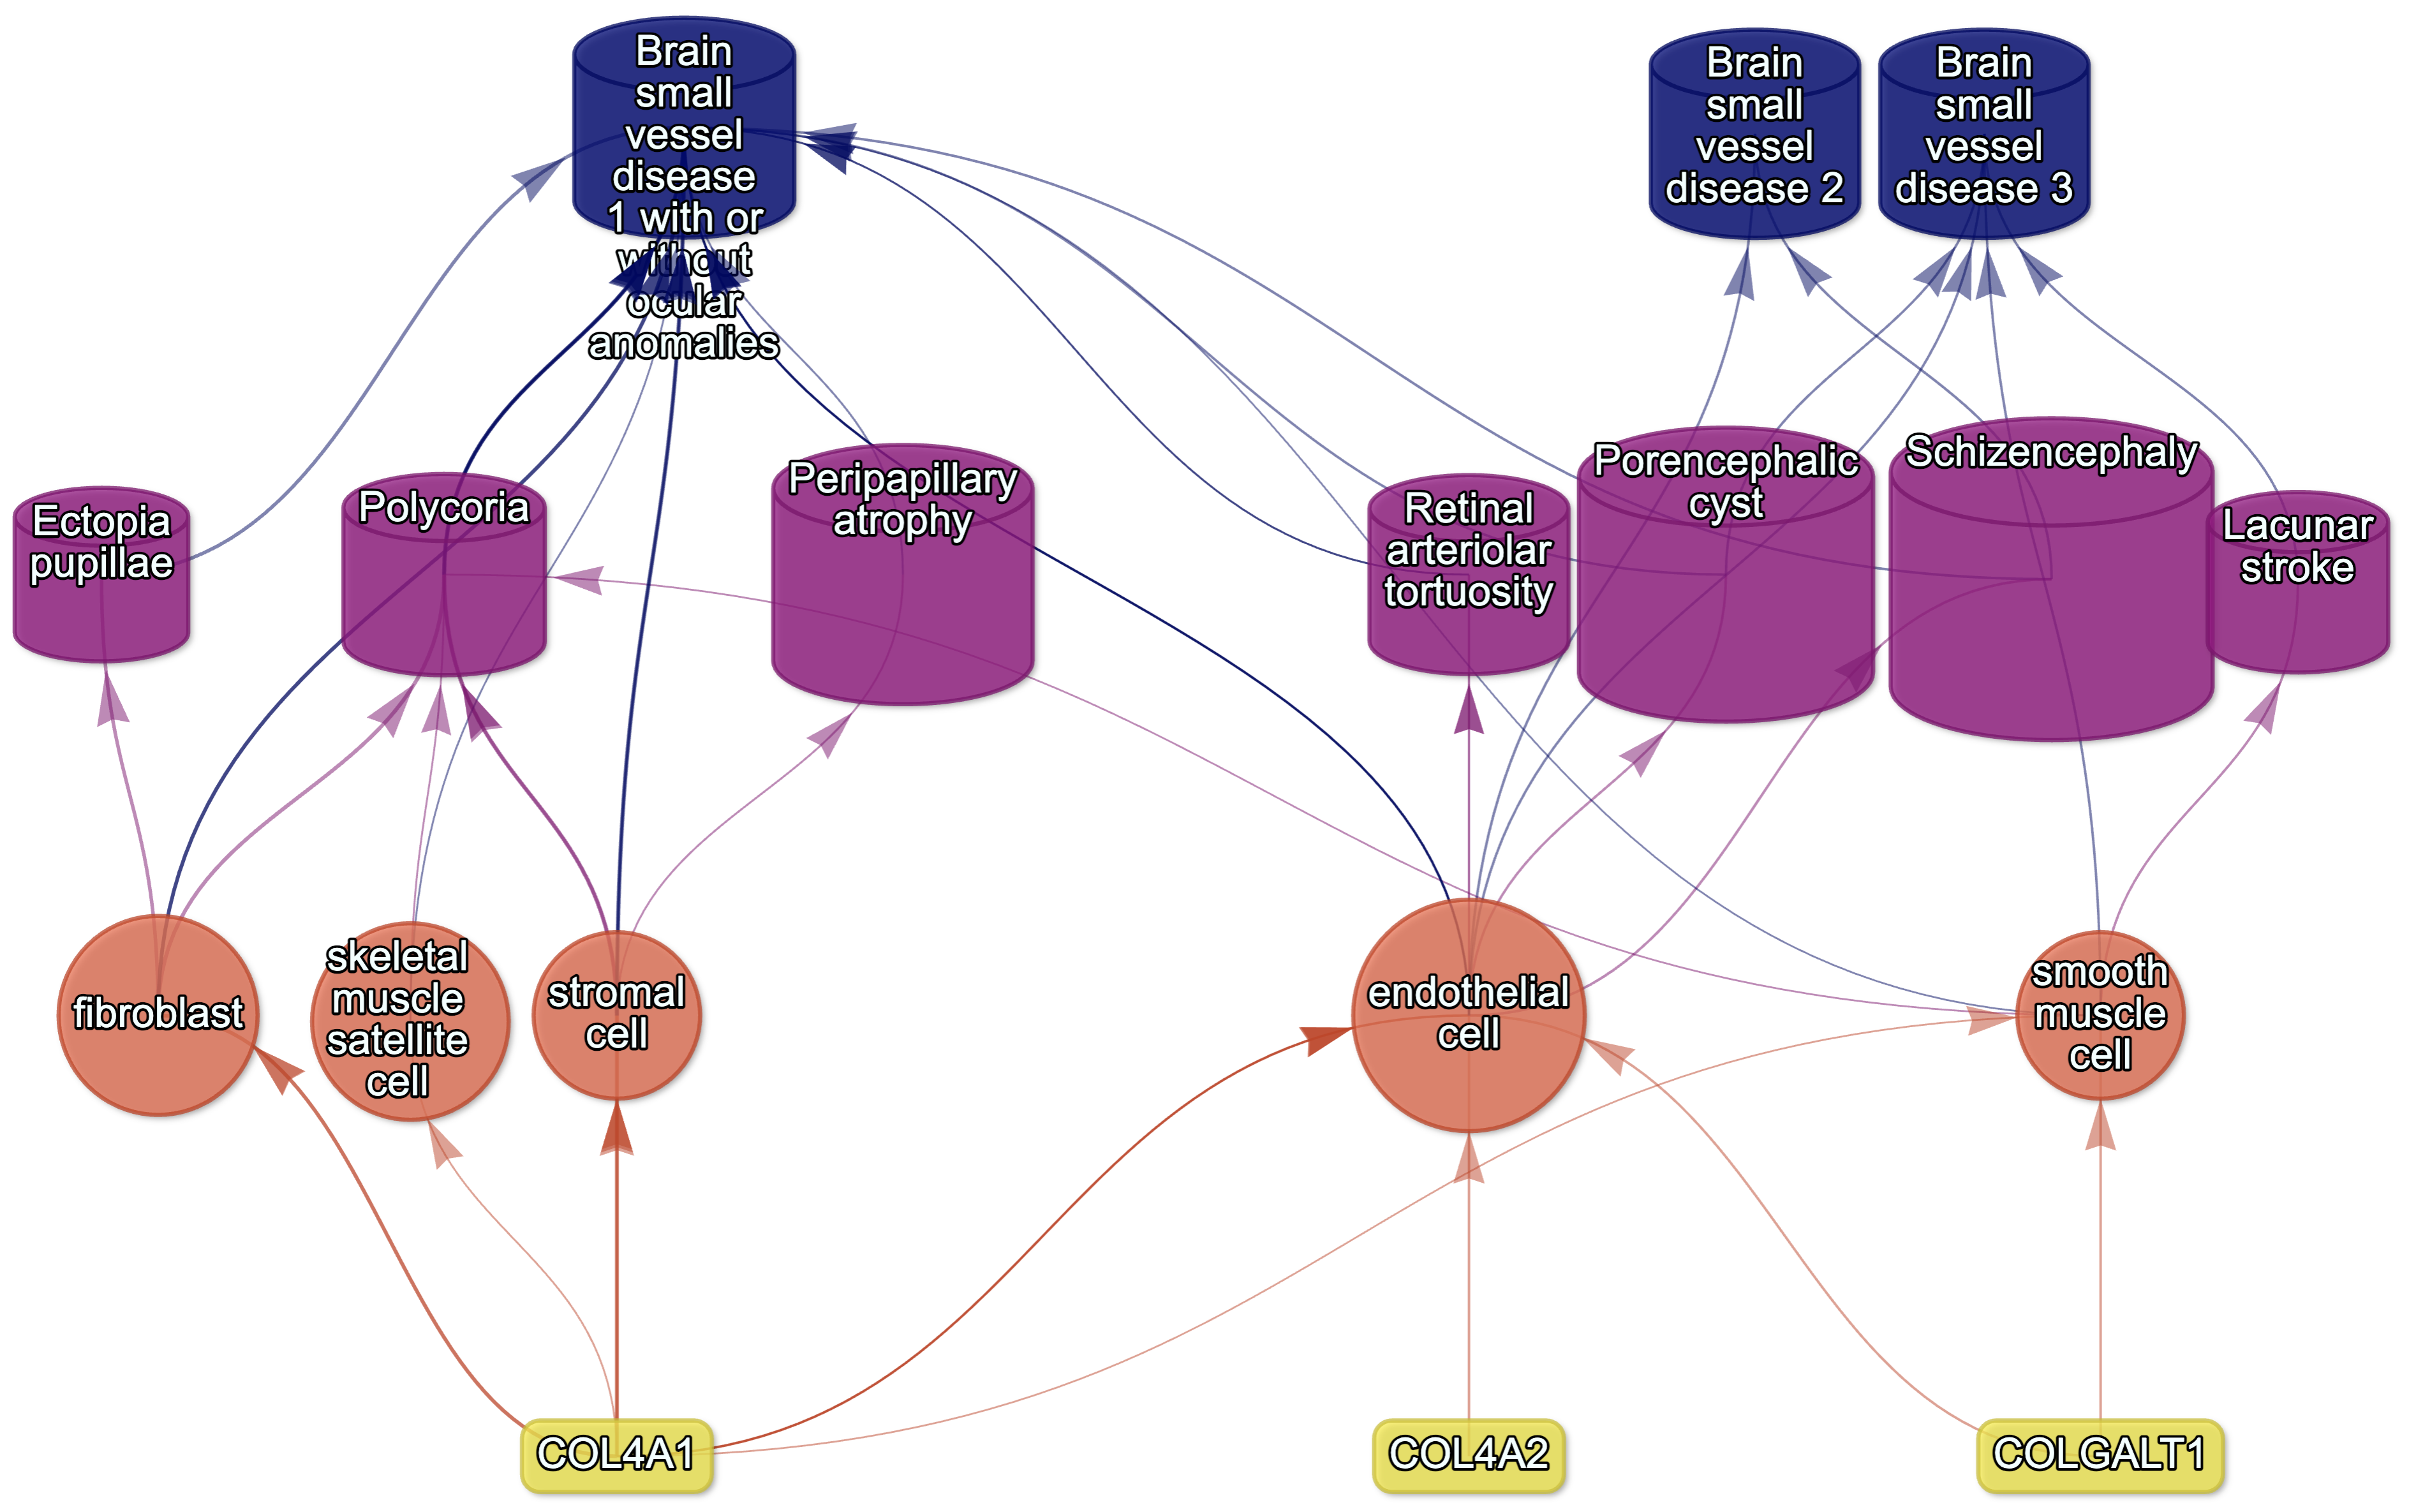
\includegraphics{img/fig-therapy-examples-supp/small_vessel_disease.png}

}

\caption{\label{fig-therapy-examples-supp-e}Small vessel disease}

\end{figure}%

\newpage{}

\begin{figure}

\centering{

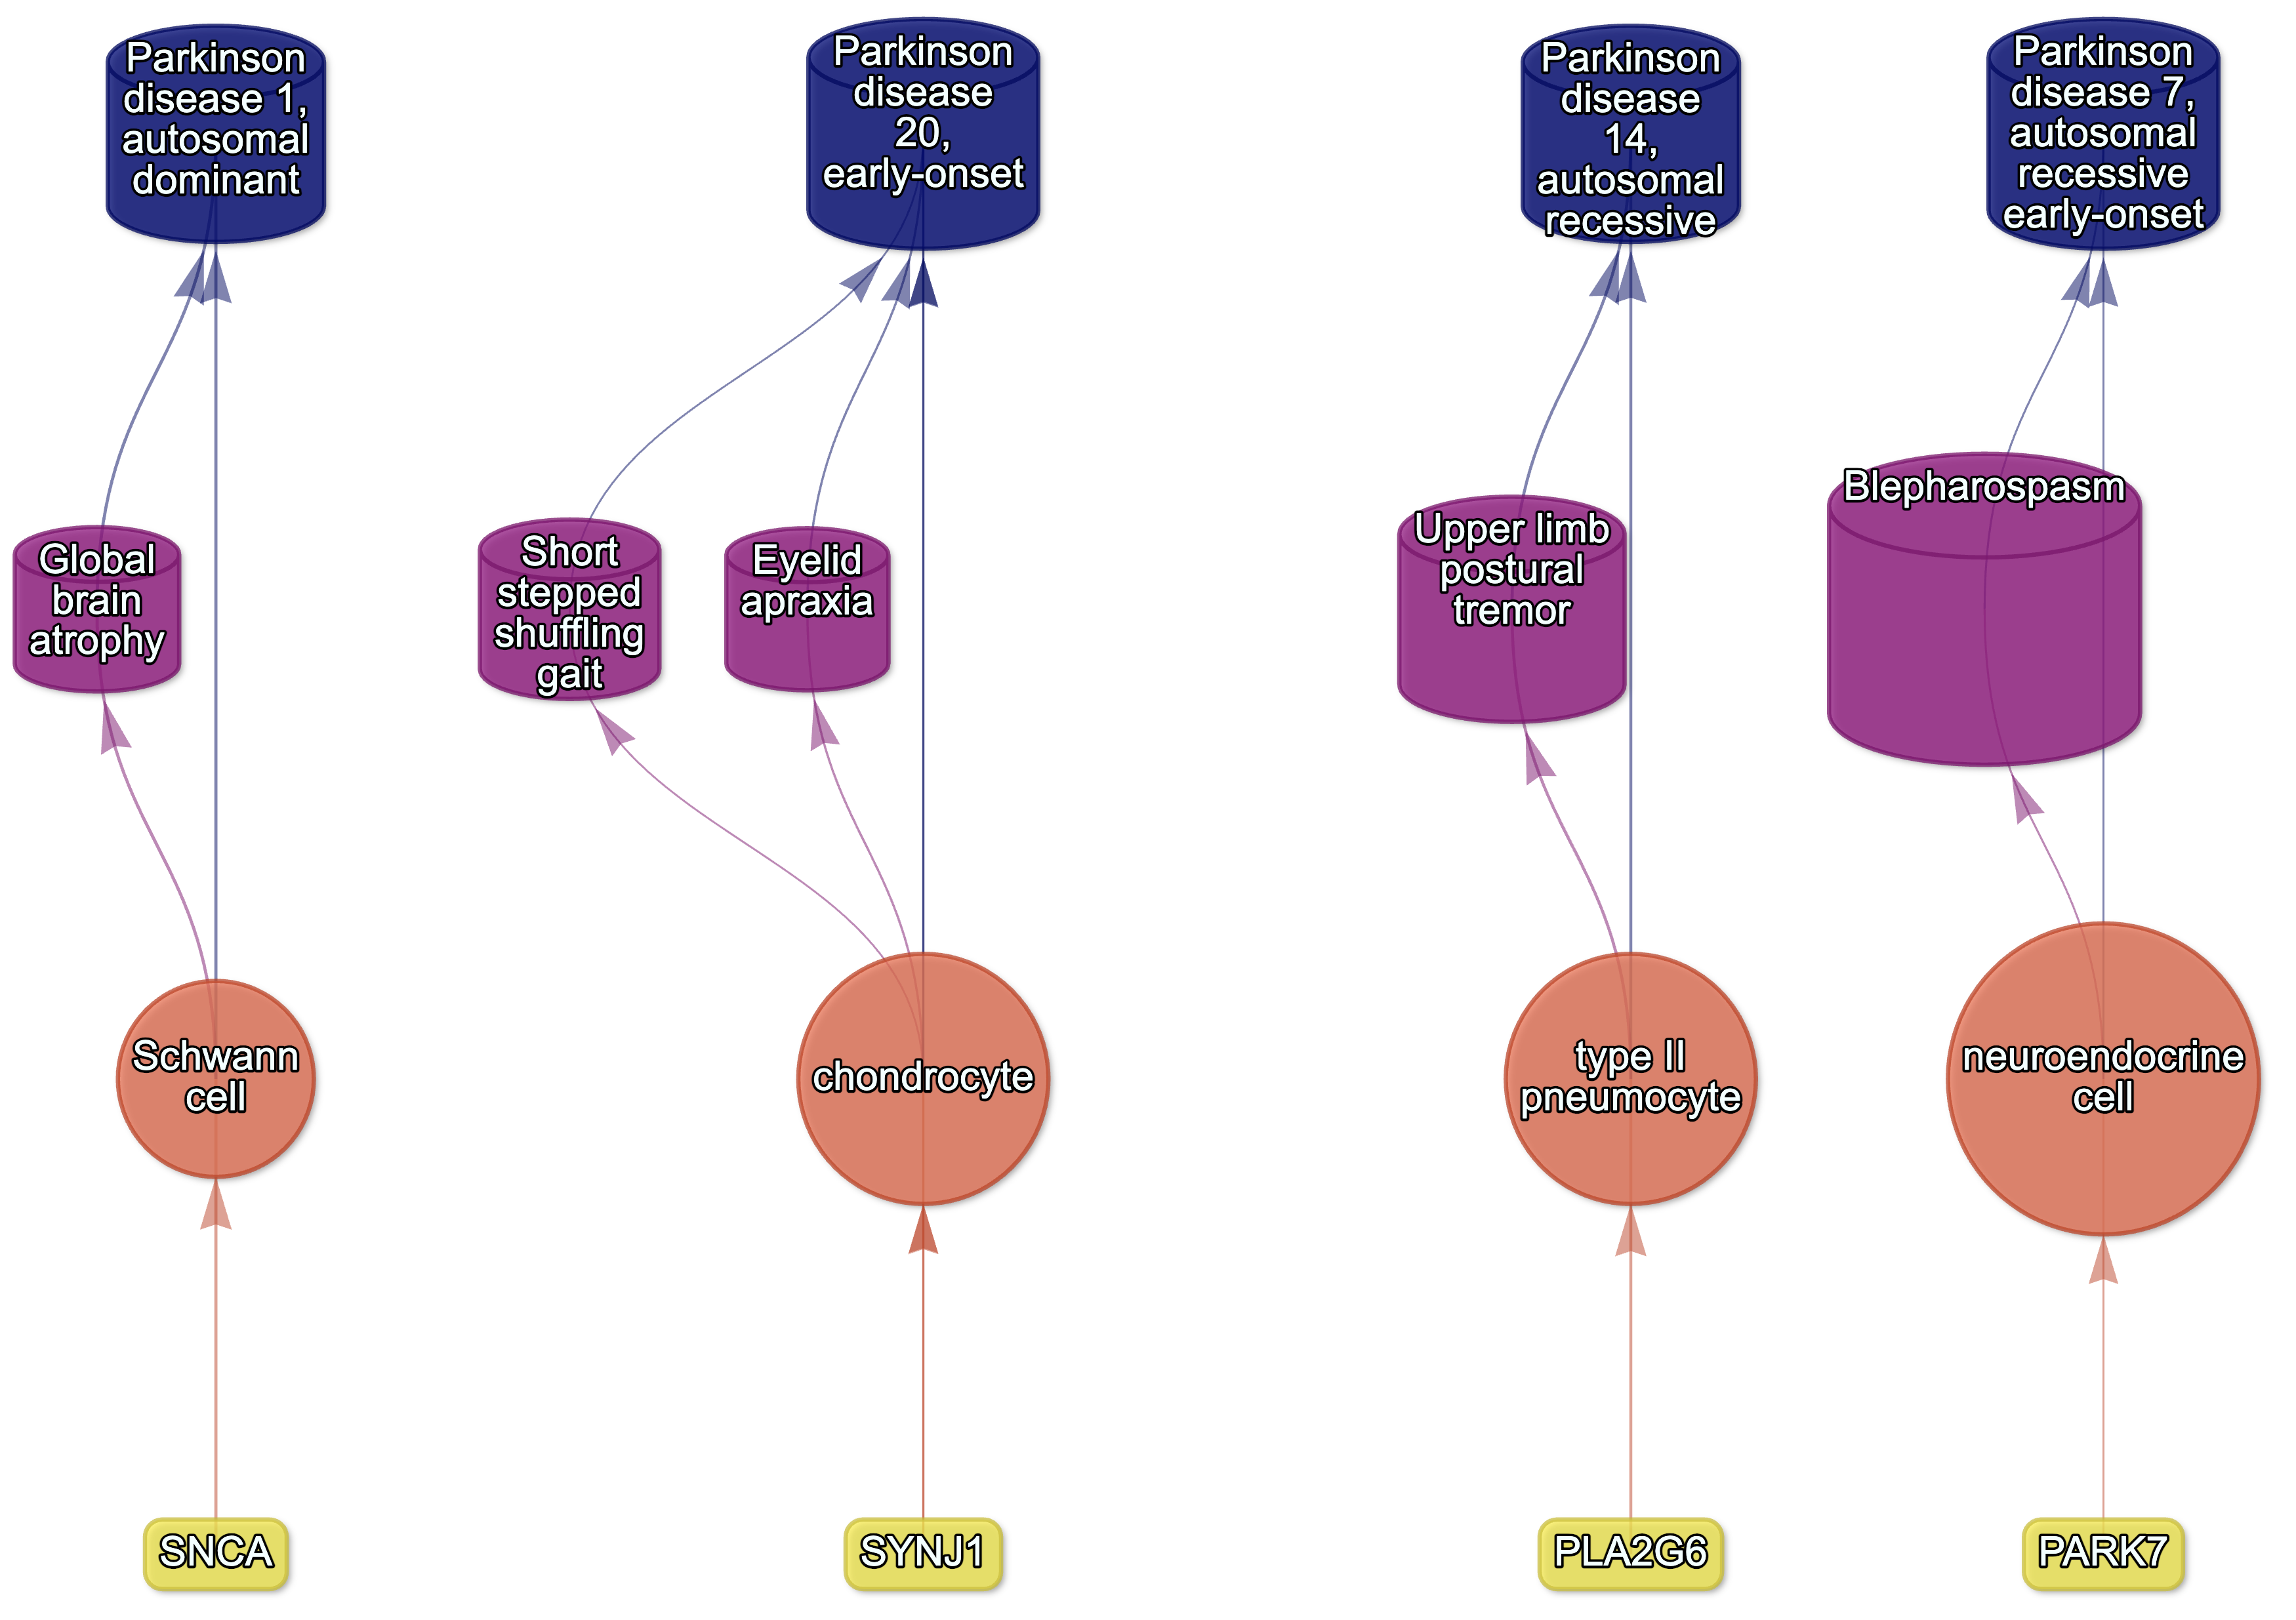
\includegraphics{img/fig-therapy-examples-supp/parkinson.png}

}

\caption{\label{fig-therapy-examples-supp-f}Parkinson's disease}

\end{figure}%

\newpage{}

\begin{figure}

\centering{

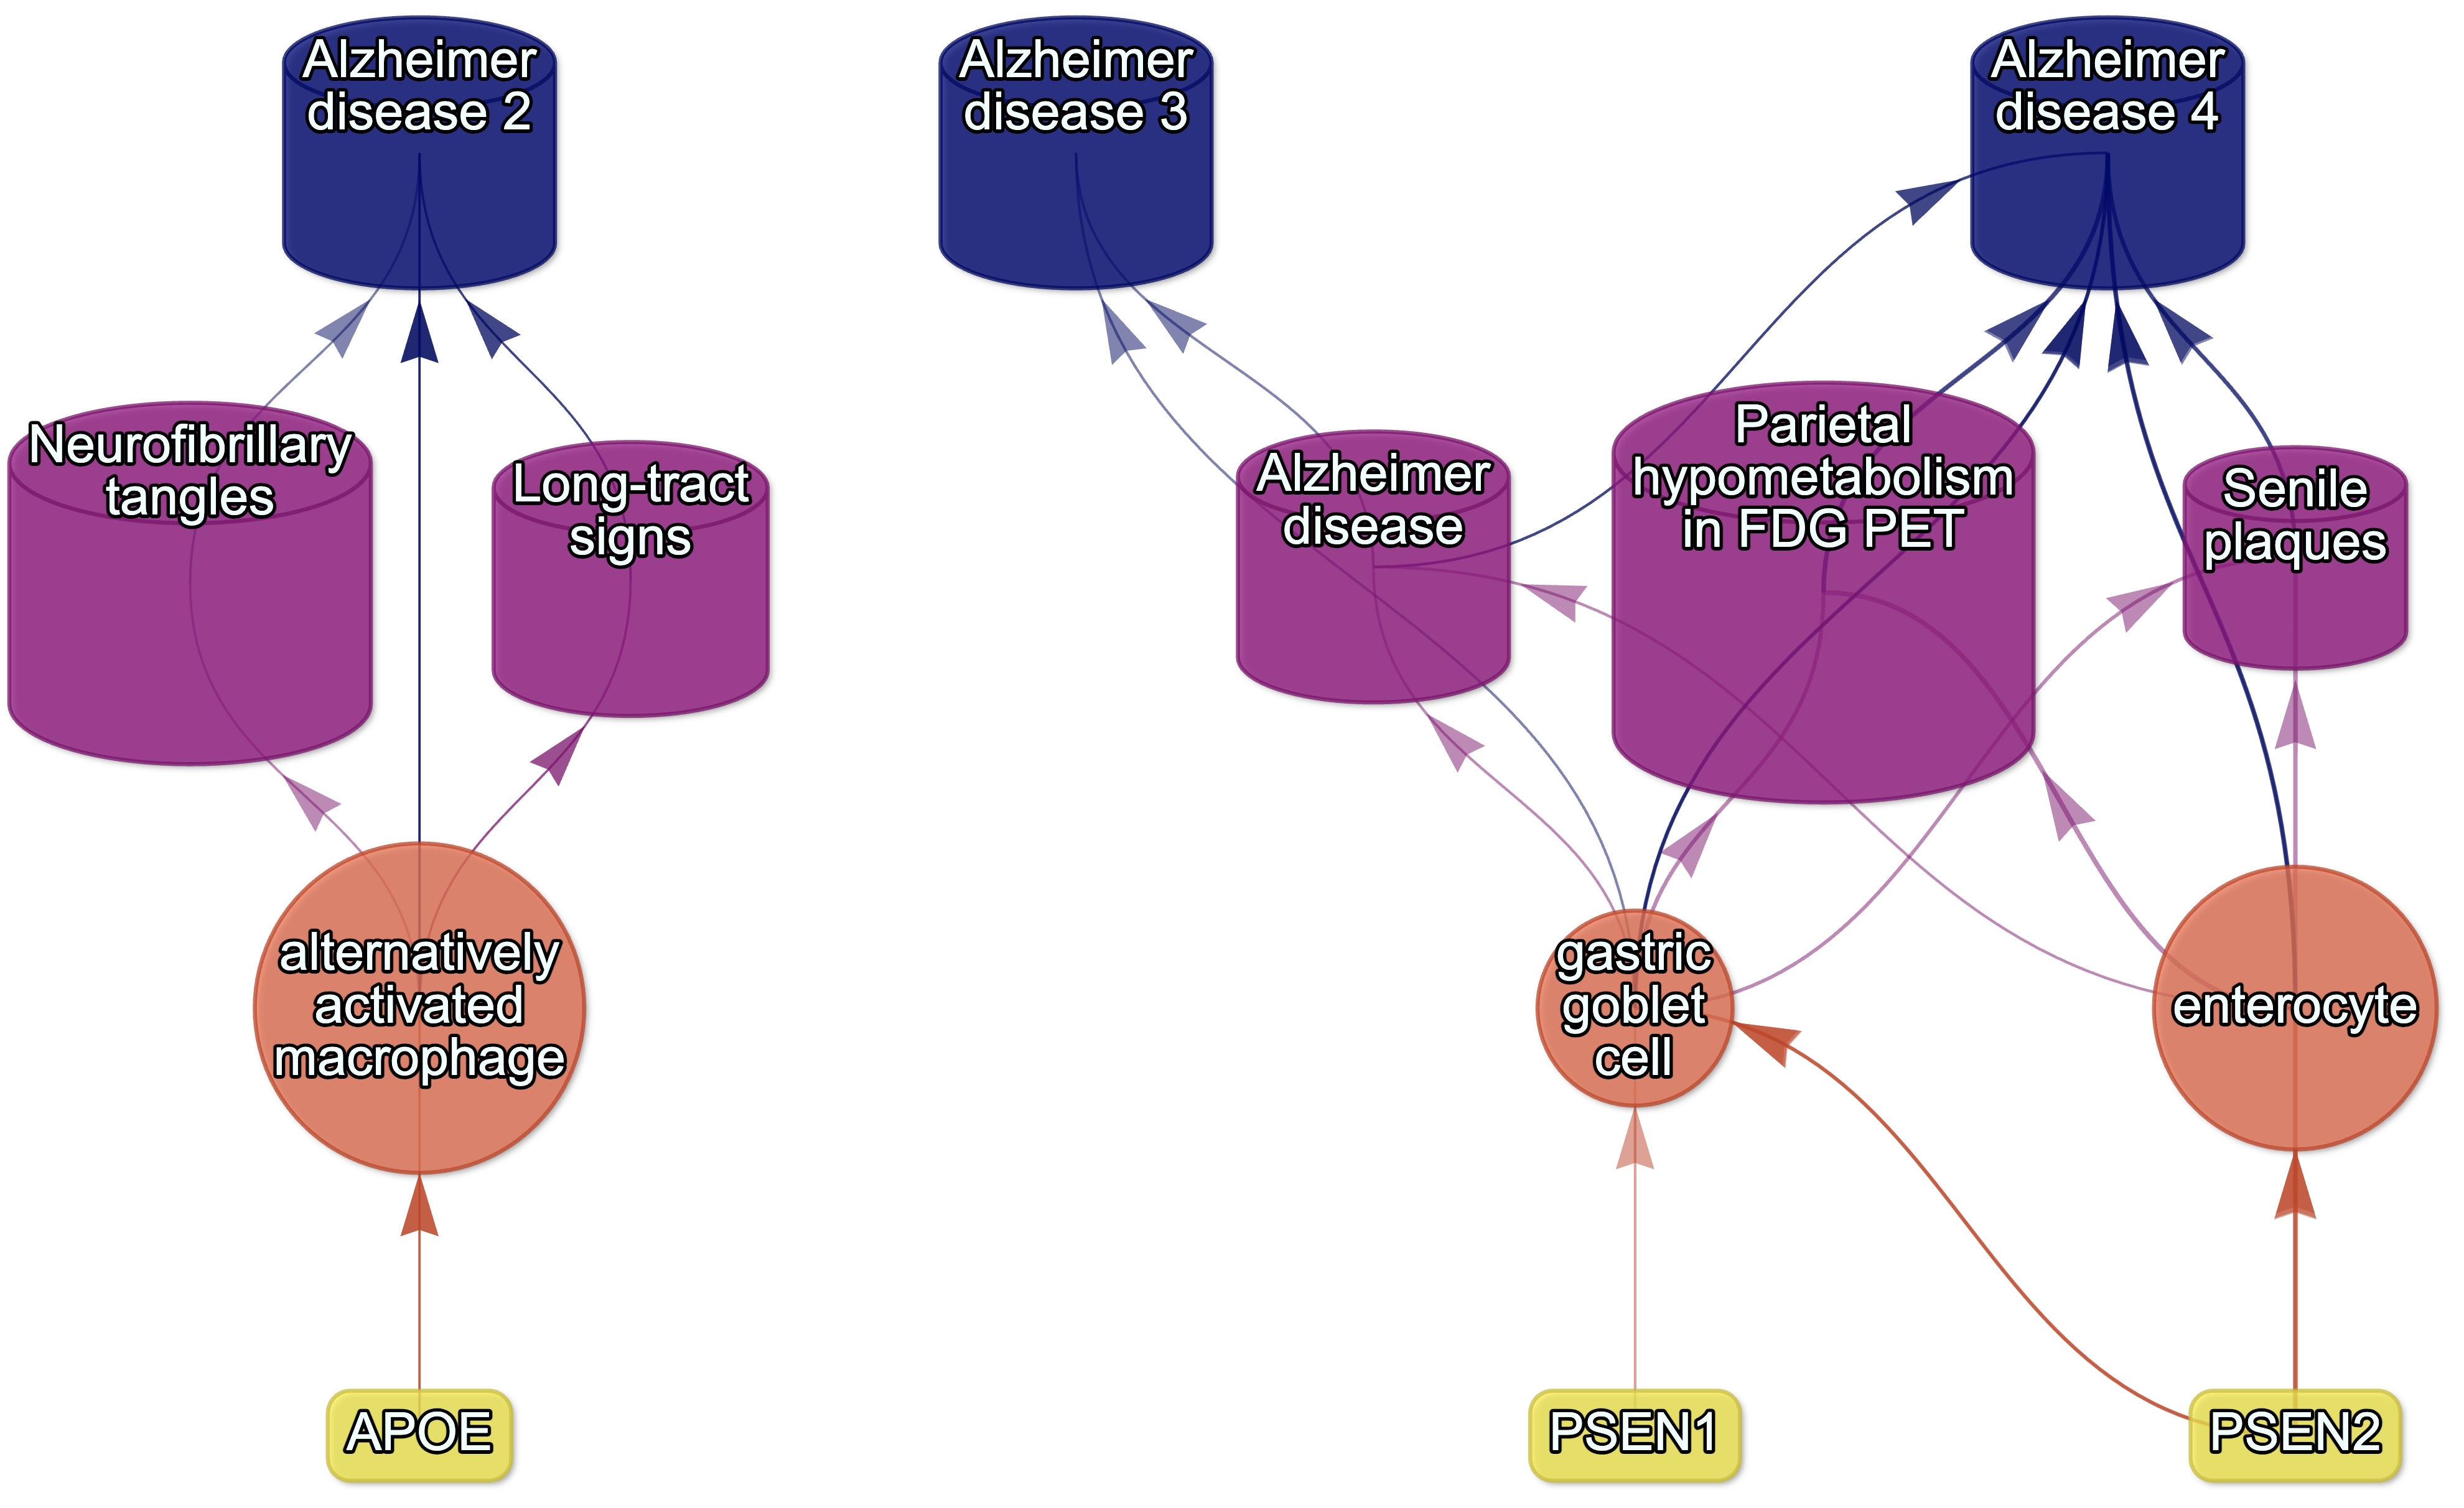
\includegraphics{img/fig-therapy-examples-supp/alzheimer.png}

}

\caption{\label{fig-therapy-examples-supp-g}Alzheimer's disease}

\end{figure}%

Example cell type-specific gene therapy targets for several severe
phenotypes and their associated diseases. Each disease (blue cylinders)
is connected to its phenotype (purple cylinders) based on
well-established clinical observations recorded within the
HPO\textsuperscript{11}.Phenotypes are connected to cell types (red
circles) via association testing between weighted gene sets
(FDR\textless0.05). Each cell type is connected to the prioritised gene
targets (yellow boxes) based on the driver gene analysis.The thickness
of the edges connecting the nodes represent the (mean) fold-change from
the bootstrapped enrichment tests. Nodes were spatially arranged using
the Sugiyama algorithm\textsuperscript{50}.

\subsection{Supplementary Tables}\label{supplementary-tables}

\begin{longtable}[]{@{}llr@{}}
\toprule\noalign{}
classification\_curie & classification\_title & encoding \\
\midrule\noalign{}
\endhead
\bottomrule\noalign{}
\endlastfoot
GENCC:100001 & Definitive & 6 \\
GENCC:100002 & Strong & 5 \\
GENCC:100003 & Moderate & 4 \\
GENCC:100009 & Supportive & 3 \\
GENCC:100004 & Limited & 2 \\
GENCC:100005 & Disputed Evidence & 1 \\
GENCC:100008 & No Known Disease Relationship & 0 \\
GENCC:100006 & Refuted Evidence & 0 \\
\end{longtable}

\newpage{}

\begin{longtable}[]{@{}
  >{\raggedright\arraybackslash}p{(\columnwidth - 6\tabcolsep) * \real{0.2800}}
  >{\raggedright\arraybackslash}p{(\columnwidth - 6\tabcolsep) * \real{0.3600}}
  >{\raggedright\arraybackslash}p{(\columnwidth - 6\tabcolsep) * \real{0.2867}}
  >{\raggedright\arraybackslash}p{(\columnwidth - 6\tabcolsep) * \real{0.0733}}@{}}
\toprule\noalign{}
\begin{minipage}[b]{\linewidth}\raggedright
hpo\_branch
\end{minipage} & \begin{minipage}[b]{\linewidth}\raggedright
cl\_branch
\end{minipage} & \begin{minipage}[b]{\linewidth}\raggedright
cl\_name
\end{minipage} & \begin{minipage}[b]{\linewidth}\raggedright
cl\_id
\end{minipage} \\
\midrule\noalign{}
\endhead
\bottomrule\noalign{}
\endlastfoot
Abnormality of the cardiovascular system & cardiocyte & cardiac muscle
cell & CL:0000746 \\
Abnormality of the cardiovascular system & cardiocyte & regular atrial
cardiac myocyte & CL:0002129 \\
Abnormality of the cardiovascular system & cardiocyte & endocardial cell
& CL:0002350 \\
Abnormality of the cardiovascular system & cardiocyte & epicardial
adipocyte & CL:1000309 \\
Abnormality of the cardiovascular system & cardiocyte & ventricular
cardiac muscle cell & CL:2000046 \\
Abnormality of the endocrine system & endocrine cell & endocrine cell &
CL:0000163 \\
Abnormality of the endocrine system & endocrine cell & neuroendocrine
cell & CL:0000165 \\
Abnormality of the endocrine system & endocrine cell & chromaffin cell &
CL:0000166 \\
Abnormality of the eye & photoreceptor cell / retinal cell &
photoreceptor cell & CL:0000210 \\
Abnormality of the eye & photoreceptor cell / retinal cell & amacrine
cell & CL:0000561 \\
Abnormality of the eye & photoreceptor cell / retinal cell & Mueller
cell & CL:0000636 \\
Abnormality of the eye & photoreceptor cell / retinal cell & retinal
pigment epithelial cell & CL:0002586 \\
Abnormality of the immune system & leukocyte & T cell & CL:0000084 \\
Abnormality of the immune system & leukocyte & mature neutrophil &
CL:0000096 \\
Abnormality of the immune system & leukocyte & mast cell & CL:0000097 \\
Abnormality of the immune system & leukocyte & microglial cell &
CL:0000129 \\
Abnormality of the immune system & leukocyte & professional antigen
presenting cell & CL:0000145 \\
Abnormality of the immune system & leukocyte & macrophage &
CL:0000235 \\
Abnormality of the immune system & leukocyte & B cell & CL:0000236 \\
Abnormality of the immune system & leukocyte & dendritic cell &
CL:0000451 \\
Abnormality of the immune system & leukocyte & monocyte & CL:0000576 \\
Abnormality of the immune system & leukocyte & plasma cell &
CL:0000786 \\
Abnormality of the immune system & leukocyte & alternatively activated
macrophage & CL:0000890 \\
Abnormality of the immune system & leukocyte & thymocyte & CL:0000893 \\
Abnormality of the immune system & leukocyte & innate lymphoid cell &
CL:0001065 \\
Abnormality of the musculoskeletal system & cell of skeletal muscle /
chondrocyte & chondrocyte & CL:0000138 \\
Abnormality of the musculoskeletal system & cell of skeletal muscle /
chondrocyte & cell of skeletal muscle & CL:0000188 \\
Abnormality of the musculoskeletal system & cell of skeletal muscle /
chondrocyte & skeletal muscle satellite cell & CL:0000594 \\
Abnormality of the nervous system & neural cell & bipolar neuron &
CL:0000103 \\
Abnormality of the nervous system & neural cell & granule cell &
CL:0000120 \\
Abnormality of the nervous system & neural cell & Purkinje cell &
CL:0000121 \\
Abnormality of the nervous system & neural cell & glial cell &
CL:0000125 \\
Abnormality of the nervous system & neural cell & astrocyte &
CL:0000127 \\
Abnormality of the nervous system & neural cell & oligodendrocyte &
CL:0000128 \\
Abnormality of the nervous system & neural cell & microglial cell &
CL:0000129 \\
Abnormality of the nervous system & neural cell & neuroendocrine cell &
CL:0000165 \\
Abnormality of the nervous system & neural cell & chromaffin cell &
CL:0000166 \\
Abnormality of the nervous system & neural cell & photoreceptor cell &
CL:0000210 \\
Abnormality of the nervous system & neural cell & inhibitory interneuron
& CL:0000498 \\
Abnormality of the nervous system & neural cell & neuron & CL:0000540 \\
Abnormality of the nervous system & neural cell & neuronal brush cell &
CL:0000555 \\
Abnormality of the nervous system & neural cell & amacrine cell &
CL:0000561 \\
Abnormality of the nervous system & neural cell & GABAergic neuron &
CL:0000617 \\
Abnormality of the nervous system & neural cell & Mueller cell &
CL:0000636 \\
Abnormality of the nervous system & neural cell & glutamatergic neuron &
CL:0000679 \\
Abnormality of the nervous system & neural cell & retinal ganglion cell
& CL:0000740 \\
Abnormality of the nervous system & neural cell & retina horizontal cell
& CL:0000745 \\
Abnormality of the nervous system & neural cell & Schwann cell &
CL:0002573 \\
Abnormality of the nervous system & neural cell & retinal pigment
epithelial cell & CL:0002586 \\
Abnormality of the nervous system & neural cell & visceromotor neuron &
CL:0005025 \\
Abnormality of the nervous system & neural cell & sympathetic neuron &
CL:0011103 \\
Abnormality of the respiratory system & respiratory epithelial cell /
epithelial cell of lung & type II pneumocyte & CL:0002063 \\
Abnormality of the respiratory system & respiratory epithelial cell /
epithelial cell of lung & epithelial cell of lower respiratory tract &
CL:0002632 \\
\end{longtable}

\newpage{}

\begin{longtable}[]{@{}llr@{}}
\toprule\noalign{}
hpo\_id & hpo\_name & encoding \\
\midrule\noalign{}
\endhead
\bottomrule\noalign{}
\endlastfoot
HP:0003826 & Stillbirth & 1 \\
HP:0005268 & Miscarriage & 1 \\
HP:0034241 & Prenatal death & 1 \\
HP:0003811 & Neonatal death & 2 \\
HP:0001522 & Death in infancy & 3 \\
HP:0003819 & Death in childhood & 4 \\
HP:0011421 & Death in adolescence & 5 \\
HP:0100613 & Death in early adulthood & 6 \\
HP:0033763 & Death in adulthood & 7 \\
HP:0033764 & Death in middle age & 7 \\
HP:0033765 & Death in late adulthood & 8 \\
\end{longtable}




\end{document}
